%% Supplementary Information — standalone document
%% Compilation: pdflatex supplemental && bibtex supplemental && pdflatex supplemental && pdflatex supplemental

\documentclass[preprint,12pt,authoryear]{elsarticle}

\usepackage{amsmath,amssymb}
\usepackage{booktabs}
\usepackage{graphicx}
\usepackage{subcaption}
\usepackage{hyperref}
\usepackage{xcolor}
\usepackage{multirow}
\usepackage[version=4]{mhchem}
\usepackage{siunitx}
\usepackage[left=1.5cm, right=1.5cm, top=2.5cm, bottom=2.5cm]{geometry}
\usepackage[section]{placeins}
\usepackage{float}
\usepackage{longtable}

%% S-prefix numbering throughout
\setcounter{section}{0}
\setcounter{figure}{0}
\setcounter{table}{0}
\setcounter{equation}{0}
\renewcommand{\thesection}{S\arabic{section}}
\renewcommand{\thesubsection}{S\arabic{section}.\arabic{subsection}}
\renewcommand{\thefigure}{S\arabic{figure}}
\renewcommand{\thetable}{S\arabic{table}}
\renewcommand{\theequation}{S\arabic{equation}}

\journal{Fluid Phase Equilibria}

%% ============================================================
\begin{document}

\begin{frontmatter}

\title{Fast and Robust Phase Equilibrium Computations for CO$_2$ + H$_2$O + NaCl Mixtures
       Using the Electrolyte Cubic-Plus-Association Equation of State\\[6pt]
       \large\normalfont Supplementary Information}

\author[ohio]{Joachim Moortgat\corref{cor1}}
\author[uga]{Felipe Mour\~{a}o Coelho}
\author[rice]{Abbas Firoozabadi\corref{cor1}}
\cortext[cor1]{Corresponding authors. Email addresses: moortgat.1@osu.edu (J.\ Moortgat), af25@rice.edu (A.\ Firoozabadi).}
\affiliation[ohio]{organization={School of Earth Sciences, The Ohio State University},
             addressline={125 South Oval Mall},
             city={Columbus},
             state={OH},
             postcode={43201},
             country={USA}}
\affiliation[uga]{organization={Universit\'{e} Grenoble Alpes},
             addressline={LIPhy},
             city={Grenoble},
             postcode={38000},
             country={France}}
\affiliation[rice]{organization={Rice University},
             city={Houston},
             state={TX},
             postcode={77005},
             country={USA}}

\end{frontmatter}

%% ============================================================
\noindent
This document provides supplementary material for the main paper.
Section~S1 gives a complete nomenclature listing.
Section~S2 tabulates the CPA/eCPA equation-of-state parameters and the coefficients
of the temperature-dependent Péneloux volume shift for H$_2$O introduced in this work.
Section~S3 derives the closed-form analytical Jacobian matrices used by the inner
Newton--Raphson solvers for the CPA and eCPA phase-fugacity calculations.
Section~S4 presents additional validation figures for CO$_2$+H$_2$O and CO$_2$+NaCl
phase equilibria, aqueous density, and the simplified flash.
Section~S5 shows supplementary convergence and efficiency figures.
Section~S6 provides the full reservoir-simulation setup and performance tables.

%% ============================================================
\section{Nomenclature}
\label{sec:nomenclature}

\noindent This section provides a complete listing of all mathematical symbols used throughout the paper.
Latin symbols are given in Table~\ref{tab:nomenclature}; Greek symbols, subscripts, and
superscripts follow in the unnumbered tables below.
Within each group, symbols are listed in alphabetical order.

\subsection*{Latin symbols}

\begin{longtable}{@{}p{0.22\textwidth}p{0.60\textwidth}p{0.12\textwidth}@{}}
  \caption{Nomenclature: all mathematical symbols used in this work.
           Latin symbols are listed below; Greek symbols, subscripts, and
           superscripts follow in the unnumbered tables at the end of this section.}
  \label{tab:nomenclature}\\
  \toprule
  Symbol & Description & Units \\
  \midrule
  \endfirsthead
  \multicolumn{3}{l}{\small\tablename~\thetable{} \textit{(continued)}}\\[2pt]
  \toprule
  Symbol & Description & Units \\
  \midrule
  \endhead
  \midrule
  \multicolumn{3}{r}{\textit{continued on next page}} \\
  \endfoot
  \bottomrule
  \endlastfoot
  \multicolumn{3}{l}{\textit{Upper case}} \\[2pt]
  $A$ & Dimensionless SRK attractive parameter, $A = a(T)P/(RT)^2$ & --- \\
  $A^r$ & Residual Helmholtz energy per mole & J mol$^{-1}$ \\
  $A^{\rm assoc}$ & Wertheim association term of $A^r$ & J mol$^{-1}$ \\
  $A^{\rm Born}$ & Born solvation contribution to $A^r$ & J mol$^{-1}$ \\
  $A^{\rm DH}$ & Debye--Hückel electrostatic contribution to $A^r$ & J mol$^{-1}$ \\
  $A^{\rm SRK}$ & Soave--Redlich--Kwong contribution to $A^r$ & J mol$^{-1}$ \\
  AARE & Average absolute relative error & \% \\
  $B$ & Dimensionless SRK co-volume parameter, $B = bP/(RT)$ & --- \\
  $D_c$ & CO$_2$ association denominator & --- \\
  $D_w$ & H$_2$O association denominator & --- \\
  $F_1, F_2, F_3$ & CPA inner-solve residuals in $(Z,\chi_{\rm H_2O},\chi_{\rm CO_2})$ & --- \\
  $F_z$ & Molar fractional flow of CO$_2$ & --- \\
  $G^{\rm res}$ & Residual Gibbs energy & J mol$^{-1}$ \\
  $G_0, G_1, G_2$ & eCPA inner-solve residuals in $(Z^{\rm aq},\varepsilon_r,\chi_{\rm H_2O})$ & --- \\
  $H_{ij}$ & Jacobian entries for the eCPA $(Z^{\rm aq},\varepsilon_r,\chi_{\rm H_2O})$ system & various \\
  $J_{ij}$ & Jacobian entries for the CPA $(Z,\chi_{\rm H_2O},\chi_{\rm CO_2})$ system & various \\
  $K$ & Isotropic permeability & mD \\
  $K_i$ & Vapour--liquid K-value of species $i$, $K_i = y_i/x_i$ & --- \\
  $K_i^W$ & Wilson K-value correlation & --- \\
  $L$ & Step-size clipping limit in accelerated SSI & --- \\
  $L_x, L_y, L_z$ & Reservoir domain dimensions & m \\
  $M_w$ & Molar mass of water (0.018015\,kg\,mol$^{-1}$) & kg mol$^{-1}$ \\
  $N_A$ & Avogadro number & mol$^{-1}$ \\
  $N_x, N_y$ & Number of grid cells in $x$- and $y$-direction & --- \\
  $P$ & Pressure & bar \\
  $P_c$ & Critical pressure & bar \\
  $P_{\rm BHP}$ & Bottom-hole pressure & bar \\
  $P_{\rm sat}$ & Saturation pressure of pure H$_2$O & bar \\
  $R$ & Universal gas constant & J mol$^{-1}$ K$^{-1}$ \\
  $R_B$ & Born radius of ion & \AA \\
  $S_g$ & CO$_2$-rich phase saturation & --- \\
  $S_{{\rm CO_2},{\rm H_2O}}$ & CO$_2$--H$_2$O cross-association strength ratio & --- \\
  $S_{gr}$ & Residual gas saturation (Corey) & --- \\
  $S_{wc}$ & Connate water saturation (Corey) & --- \\
  $T$ & Temperature & $^\circ$C or K \\
  $T_c$ & Critical temperature & K \\
  $\text{TPD}(\mathbf{W})$ & Tangent-plane distance function & --- \\
  $V_g$ & Radial distribution function derivative with respect to $\eta$ & --- \\
  $W$ & Second derivative of $V_g$; also unnormalized trial composition vector & --- \\
  $Z$ & Compressibility factor, $Z = Pv/(RT)$ & --- \\
  $Z^c$ & Compressibility factor of the CO$_2$-rich phase & --- \\
  $Z^{\rm aq}$ & Compressibility factor of the aqueous phase & --- \\[4pt]
  \multicolumn{3}{l}{\textit{Lower case}} \\[2pt]
  $a(T)$ & Mixture SRK attractive parameter & J cm$^3$ mol$^{-2}$ \\
  $a_{0i}$ & Pure-component reference attractive parameter & J cm$^3$ mol$^{-2}$ \\
  $b$ & Mixture SRK co-volume parameter & cm$^3$ mol$^{-1}$ \\
  $b_i$ & Pure-component co-volume & cm$^3$ mol$^{-1}$ \\
  $c_i$ & Péneloux volume-shift parameter of species $i$ & cm$^3$ mol$^{-1}$ \\
  $c_{1i}$ & Soave temperature-dependence coefficient of species $i$ & --- \\
  $d_i$ & Reference chemical-potential offset in TPD, $\ln z_i + \ln\hat{\phi}_i(\mathbf{z})$ & --- \\
  $g(\eta)$ & Carnahan--Starling radial distribution function & --- \\
  $g_w$ & Kirkwood $g$-factor for water & --- \\
  $\mathbf{g}^{(k)}$ & Fugacity-ratio residual vector at SSI iteration $k$ & --- \\
  $k_{ij}$ & Binary interaction parameter between species $i$ and $j$ & --- \\
  $k_B$ & Boltzmann constant & J K$^{-1}$ \\
  $k_{rg}, k_{rw}$ & Corey relative permeabilities (CO$_2$-rich, aqueous) & --- \\
  $m^{(k)}$ & Dominant-eigenvalue acceleration factor at iteration $k$ & --- \\
  $m_{\text{CO}_2}$ & CO$_2$ molality in the aqueous phase & mol kg$^{-1}$ \\
  $m_s$ & NaCl feed molality (solution-table grid coordinate); no superscript = feed value & mol kg$^{-1}$ \\
  $m_s^{\rm aq}$ & Self-consistent equilibrium NaCl molality in the aqueous phase & mol kg$^{-1}$ \\
  $n_g, n_w$ & Corey exponents (CO$_2$-rich, aqueous) & --- \\
  $q$ & Well volumetric flow rate & m$^3$ s$^{-1}$ \\
  $r_w$ & Wellbore radius & m \\
  $t$ & Time & yr \\
  $v$ & Molar volume & cm$^3$ mol$^{-1}$ \\
  $w_i$ & Normalised trial mole fractions in stability test & --- \\
  $x_i$ & Mole fraction of species $i$ in the aqueous phase & --- \\
  $x_{\rm CO_2}^{\rm sf}$ & CO$_2$ mole fraction on a salt-free basis & --- \\
  $y_i$ & Mole fraction of species $i$ in the CO$_2$-rich phase & --- \\
  $\mathbf{z}$ & Overall feed composition vector, $\mathbf{z} = (z_{\rm H_2O}, z_{\rm CO_2})$ & --- \\
  $z_{\rm H_2O}$ & Overall H$_2$O feed mole fraction, $z_{\rm H_2O} = 1 - z_{\rm CO_2}$ & --- \\
  $z_{\rm CO_2}$ & Overall CO$_2$ feed mole fraction & --- \\
\end{longtable}

\subsection*{Greek symbols}

\begin{tabular}{@{}lll@{}}
  \toprule
  Symbol & Description & Units \\
  \midrule
  $\alpha_{is}$ & NRTL non-randomness parameter (ion--solvent) & --- \\
  $\beta$ & CO$_2$-rich phase molar fraction & --- \\
  $\delta^{A_iB_j}$ & Association bonding volume between sites $A_i$ and $B_j$ & m$^3$ mol$^{-1}$ \\
  $\Delta U_{is}$ & Ion--solvent interaction energy (eCPA NRTL term) & J mol$^{-1}$ \\
  $\varepsilon/k_B$ & Association well depth (temperature units) & K \\
  $\varepsilon_0$ & Vacuum permittivity & F m$^{-1}$ \\
  $\varepsilon_\infty$ & High-frequency (optical) relative permittivity & --- \\
  $\varepsilon_r$ & Static relative permittivity (dielectric constant) of water & --- \\
  $\eta$ & Packing fraction, $\eta = b/(4v)$ & --- \\
  $\hat{\phi}_i$ & Fugacity coefficient of species $i$ & --- \\
  $\kappa$ & Association volume parameter in the Wertheim term & --- \\
  $\mu_{0w}$ & Permanent dipole moment of water & C m \\
  $\mu_g, \mu_w$ & Dynamic viscosity (CO$_2$-rich, aqueous) & Pa s \\
  $\rho$ & Mass density & kg m$^{-3}$ \\
  $\rho_N$ & Molar density (mixture), $\rho_N = P/(ZRT)$ & mol m$^{-3}$ \\
  $\sigma$ & Collision diameter (ion hard-sphere radius) & \AA \\
  $\tau, \tau_{\rm switch}$ & SSI convergence tolerance; Newton-polish switch threshold & --- \\
  $\phi$ & Porosity & --- \\
  $\chi^{A_i}$ & Fraction of molecules of species $i$ not bonded at site $A$ & --- \\
  $\chi_{\rm H_2O}, \chi_{\rm CO_2}$ & Non-bonded fractions of H$_2$O and CO$_2$ & --- \\
  $\omega_i$ & Acentric factor of species $i$ & --- \\
  \bottomrule
\end{tabular}

\subsection*{Subscripts and superscripts}

\begin{tabular}{@{}ll@{}}
  \toprule
  Symbol & Meaning \\
  \midrule
  $c$ & CO$_2$-rich phase \\
  ${\rm aq}$ & Aqueous phase \\
  $i, j$ & Species index \\
  ${\rm H_2O},\,{\rm CO_2}$ & Component (H$_2$O or CO$_2$) \\
  assoc & Association contribution \\
  Born & Born solvation contribution \\
  DH & Debye--Hückel electrostatic contribution \\
  feed & Feed (overall) quantity \\
  phys & Physical (SRK) contribution \\
  res & Residual thermodynamic quantity \\
  SRK & Soave--Redlich--Kwong reference fluid \\
  $c, i$ & Critical property of species $i$ \\
  \bottomrule
\end{tabular}

%% ============================================================
\section{EoS Parameters}
\label{sec:params}

This section supplements the equation-of-state section of the main text.
For completeness, Tables~\ref{tab:pure_params} and \ref{tab:binary_params} reproduce the
key EoS parameters used in this work, all from \citet{Coelho2025}.
The coefficients of the temperature-dependent Péneloux volume shift for H$_2$O
(Eq.~\ref{eq:peneloux_poly}), introduced in this work, are given in
Table~\ref{tab:peneloux_coeffs}.

\begin{table}[H]
  \centering
  \caption{Pure-component CPA/eCPA parameters \citep{Coelho2025}.
           For ions, $a_0 = 0$. H$_2$O uses the 4C association scheme.}
  \label{tab:pure_params}
  \begin{tabular}{lccccccc}
    \toprule
    Species & $a_0$ (J\,m$^3$\,mol$^{-2}$) & $c_1$ & $b$ (cm$^3$\,mol$^{-1}$) &
              $\varepsilon/k_B$ (K) & $\kappa$ & $\sigma$ (\AA) & $R_B$ (\AA) \\
    \midrule
    H$_2$O & 0.1228 & 0.6736 & 14.52 & 2003 & $\kappa^*$ & ---   & ---   \\
    CO$_2$  & 0.3508 & 0.7602 & 27.20 & ---  & ---        & ---   & ---   \\
    Na$^+$  & 0      & ---    & 16.49 & ---  & ---        & 2.356 & 1.665 \\
    Cl$^-$  & 0      & ---    & 40.83 & ---  & ---        & 3.187 & 1.828 \\
    \bottomrule
  \end{tabular}
  \begin{flushleft}
    \footnotesize $^*\kappa = \kappa_{\text{assoc}} \cdot b_{\text{H}_2\text{O}}$,
    $\kappa_{\text{assoc}} = 69.2 \times 10^{-3}$.
  \end{flushleft}
\end{table}

\begin{table}[H]
  \centering
  \caption{Temperature-dependent binary interaction parameters \citep{Coelho2025}.
           $X = A_X(T/T_{c,{\rm CO_2}})^2 + B_X(T/T_{c,{\rm CO_2}}) + C_X$, $T_{c,{\rm CO_2}} = 31.3\,^\circ$C.}
  \label{tab:binary_params}
  \begin{tabular}{lrrr}
    \toprule
    Parameter & $A$ & $B$ & $C$ \\
    \midrule
    $k_{{\rm CO_2},{\rm H_2O}}$ (CO$_2$--H$_2$O binary interaction parameter) & $-0.492$ & $2.101$ & $-1.571$ \\
    $S_{{\rm CO_2},{\rm H_2O}}$ (cross-assoc.\ strength) & $+0.192$ & $-0.173$ & $-0.009$ \\
    \bottomrule
  \end{tabular}

  \vspace{6pt}
  \begin{tabular}{lrrrr}
    \toprule
    Ion--neutral pair & $\Delta U^{\text{ref}}$ (J\,mol$^{-1}$) & $\alpha$ (K) & $T^\alpha$ (K) & Source \\
    \midrule
    H$_2$O--NaCl ($\Delta U_{ws}$) & $-1858$ & 1573 & 340 & Maribo-Mogensen et al.\ (2015) \\
    CO$_2$--NaCl ($\Delta U_{cs}$) & $+6056$ & 692  & 244 & \citet{Coelho2025} \\
    \bottomrule
  \end{tabular}
\end{table}

\subsection*{Temperature-dependent Péneloux shift for H$_2$O}
\label{sec:peneloux_coeffs}

A temperature-dependent volume shift for H$_2$O is introduced in this work.
We fit a degree-4 polynomial in the reduced temperature
$T_R = T / T_{c,\text{H}_2\text{O}}$ ($T_{c,\text{H}_2\text{O}} = 647.29$\,K)
to 455 IAPWS-95 liquid/compressed-water conditions
($T = 0$--$350\,^\circ$C, $P = 1$--$2000$\,bar):
\begin{equation}
  c_{\text{H}_2\text{O}}(T) = a_4 T_R^4 + a_3 T_R^3 + a_2 T_R^2 + a_1 T_R + a_0
  \quad [\text{cm}^3\,\text{mol}^{-1}].
  \label{eq:peneloux_poly}
\end{equation}
The fitted coefficients are given in Table~\ref{tab:peneloux_coeffs}.

\begin{table}[H]
  \centering
  \caption{Coefficients of the degree-4 Péneloux volume shift polynomial for H$_2$O
           (Eq.~\ref{eq:peneloux_poly}), fitted in this work to 455 IAPWS-95 liquid/compressed-water
           conditions ($T = 0$--$350\,^\circ$C, $P = 1$--$2000$\,bar).}
  \label{tab:peneloux_coeffs}
  \begin{tabular}{cr}
    \toprule
    Coefficient & Value \\
    \midrule
    $a_4$ & $+32.862$ \\
    $a_3$ & $-96.052$ \\
    $a_2$ & $+110.954$ \\
    $a_1$ & $-58.111$ \\
    $a_0$ & $+11.233$ \\
    \bottomrule
  \end{tabular}
\end{table}

%% ============================================================
\section{Analytical Jacobians for the Inner Newton Solvers}
\label{sec:jacobians}

This section supplements the SSI and K-value flash sections of the main text,
which describe the inner Newton--Raphson solvers used at each SSI iteration to evaluate
the CPA and eCPA phase fugacities.
Here we derive the full analytical Jacobian matrices that make those Newton steps
computationally efficient.
Within each SSI iteration two distinct Newton systems are solved, one per phase.
The CO$_2$-rich phase and both phases of the salt-free CPA binary use a
$3\times 3$ system in $(Z,\chi_{\rm H_2O},\chi_{\rm CO_2})$ (Section~\ref{sec:jac_cpa}).
The eCPA aqueous phase requires a different $3\times 3$ system in
$(Z^{\rm aq},\varepsilon_r,\chi_{\rm H_2O})$, because the relative permittivity $\varepsilon_r$
satisfies an additional Kirkwood self-consistency equation
(Section~\ref{sec:jac_ecpa}).

%% ----------------------------------------------------------------
\subsection{CPA binary: Newton system for $(Z,\,\chi_{\rm H_2O},\,\chi_{\rm CO_2})$}
\label{sec:jac_cpa}

The system is written for the aqueous phase (mole fractions $x_i$); the CO$_2$-rich phase
uses the identical equations with $y_i$ in place of $x_i$.
The three fixed-point residuals are
\begin{align}
  F_1 &= Z - \frac{Z}{Z-B} + \frac{A}{Z+B}
         - G\bigl[x_{\rm H_2O}(\chi_{\rm H_2O}-1)+x_{\rm CO_2}(\chi_{\rm CO_2}-1)\bigr] = 0,
         \label{eq:F1jac} \\
  F_2 &= \chi_{\rm H_2O} - \frac{Z}{D_w} = 0,
         \label{eq:F2jac} \\
  F_3 &= \chi_{\rm CO_2} - \frac{Z}{D_c} = 0,
         \label{eq:F3jac}
\end{align}
with the denominators
\begin{equation}
  D_w = Z + 2x_{\rm H_2O}\chi_{\rm H_2O}\Delta_w + 2x_{\rm CO_2}\chi_{\rm CO_2}\Delta_{{\rm CO_2},{\rm H_2O}}, \qquad
  D_c = Z + 2x_{\rm H_2O}\chi_{\rm H_2O}\Delta_{{\rm CO_2},{\rm H_2O}},
  \label{eq:DwDc}
\end{equation}
where $\Delta_w = g(\eta)\kappa_w[\exp(\varepsilon_w/k_BT)-1]P/(RT)$,
$\Delta_{{\rm CO_2},{\rm H_2O}} = S_{{\rm CO_2},{\rm H_2O}}\Delta_w$, $\eta = B/(2Z)$,
and $G = 1 + V_g$ with
\begin{equation}
  V_g \equiv \frac{\eta g'(\eta)}{g(\eta)} = \frac{\eta(5-2\eta)}{(1-\eta)(2-\eta)}, \qquad
  W  \equiv \frac{\mathrm{d}V_g}{\mathrm{d}\eta} = \frac{10-8\eta+\eta^2}{(1-\eta)^2(2-\eta)^2},
  \label{eq:VgW}
\end{equation}
for the Carnahan--Starling radial distribution function
$g(\eta) = (2-\eta)/[2(1-\eta)^3]$.
Because $\eta \propto Z^{-1}$, the key identity is
\begin{equation}
  Z\,\frac{\partial\Delta_w}{\partial Z} = -V_g\,\Delta_w,
  \label{eq:dDeltadZ}
\end{equation}
from which all $Z$-derivatives of $D_w$ and $D_c$ follow.
Setting $D = x_{\rm H_2O}(\chi_{\rm H_2O}-1)+x_{\rm CO_2}(\chi_{\rm CO_2}-1)$, the $3\times 3$ Jacobian
$J_{ij} = \partial F_i/\partial v_j$ with $\mathbf{v}=(Z,\chi_{\rm H_2O},\chi_{\rm CO_2})^\top$ is:

\paragraph{Row 1}
\begin{align}
  J_{11} &= 1 + \frac{B}{(Z-B)^2} - \frac{A}{(Z+B)^2} + \frac{D\,W\eta}{Z},
             \label{eq:J11} \\
  J_{12} &= -G\,x_{\rm H_2O}, \label{eq:J12} \\
  J_{13} &= -G\,x_{\rm CO_2}. \label{eq:J13}
\end{align}

\paragraph{Row 2}
Using $Z\partial D_w/\partial Z = Z - 2(x_{\rm H_2O}\chi_{\rm H_2O} + x_{\rm CO_2}\chi_{\rm CO_2} S_{{\rm CO_2},{\rm H_2O}})V_g\Delta_w$
and $\chi_{\rm H_2O} = Z/D_w$:
\begin{align}
  J_{21} &= -\frac{2\Delta_w(1+V_g)(x_{\rm H_2O}\chi_{\rm H_2O} + x_{\rm CO_2}\chi_{\rm CO_2} S_{{\rm CO_2},{\rm H_2O}})}{D_w^2},
             \label{eq:J21} \\
  J_{22} &= 1 + \frac{2x_{\rm H_2O}\Delta_w\chi_{\rm H_2O}}{D_w}, \label{eq:J22} \\
  J_{23} &= \frac{2x_{\rm CO_2} S_{{\rm CO_2},{\rm H_2O}}\Delta_w\chi_{\rm H_2O}}{D_w}. \label{eq:J23}
\end{align}

\paragraph{Row 3}
Using $Z\partial D_c/\partial Z = Z - 2x_{\rm H_2O}\chi_{\rm H_2O} S_{{\rm CO_2},{\rm H_2O}} V_g\Delta_w$
and $\chi_{\rm CO_2} = Z/D_c$:
\begin{align}
  J_{31} &= -\frac{2x_{\rm H_2O}\chi_{\rm H_2O} S_{{\rm CO_2},{\rm H_2O}}\Delta_w(1+V_g)}{D_c^2},
             \label{eq:J31} \\
  J_{32} &= \frac{2x_{\rm H_2O} S_{{\rm CO_2},{\rm H_2O}}\Delta_w\chi_{\rm CO_2}}{D_c}, \label{eq:J32} \\
  J_{33} &= 1. \label{eq:J33}
\end{align}
Note $J_{33}=1$ because $D_c$ does not depend on $\chi_{\rm CO_2}$; Newton therefore
has a direct update for $\chi_{\rm CO_2}$ at each step.
For the CO$_2$-rich phase the identical Jacobian applies with $y_i$ in place of $x_i$.

%% ----------------------------------------------------------------
\subsection{eCPA aqueous phase: Newton system for $(Z^{\rm aq},\,\varepsilon_r,\,\chi_{\rm H_2O})$}
\label{sec:jac_ecpa}

In the aqueous phase the relative permittivity $\varepsilon_r$ is an additional
unknown satisfying the Kirkwood self-consistency equation~\eqref{eq:G1}.
The CO$_2$ cross-association fraction $\chi_{\rm CO_2}$ is eliminated algebraically via
$\chi_{\rm CO_2} = Z^{\rm aq}/D_c$ with $D_c = Z^{\rm aq} + 2x_{\rm H_2O}\chi_{\rm H_2O} S_{{\rm CO_2},{\rm H_2O}}\Delta_w$, reducing the
system to three equations in $\mathbf{v}=(Z^{\rm aq},\varepsilon_r,\chi_{\rm H_2O})^\top$:
\begin{align}
  G_0 &= Z^{\rm aq} - Z^{{\rm aq},\text{phys}} - Z^{{\rm aq},\text{assoc}}
              - Z^{{\rm aq},\text{DH}} - Z^{{\rm aq},\text{Perm}} = 0, \label{eq:G0} \\
  G_1 &= T_1(\varepsilon_r,\varepsilon_\infty)
        - T_2(Z^{\rm aq},\chi_{\rm H_2O}) = 0, \label{eq:G1} \\
  G_2 &= \chi_{\rm H_2O} - \frac{Z^{\rm aq}}{D_w} = 0, \label{eq:G2}
\end{align}
where $T_1$ and $T_2$ are the left- and right-hand sides of the
Onsager--Kirkwood relative permittivity fixed-point equation \citep{Coelho2025},
$D_w = Z^{\rm aq} + 2x_{\rm H_2O}\chi_{\rm H_2O}\Delta_w + 2x_{\rm CO_2}\chi_{\rm CO_2} S_{{\rm CO_2},{\rm H_2O}}\Delta_w$, and all
$Z^{\rm aq}$-derivatives of $\Delta_w$ satisfy the same identity~\eqref{eq:dDeltadZ}
(with $Z^{\rm aq}$ in place of $Z$).

\paragraph{Row 2 (exact)}
$G_2$ has the same structure as $F_2$~\eqref{eq:F2jac} with $\varepsilon_r$
absent from $D_w$, so
\begin{align}
  H_{20} &= -\frac{2\Delta_w(1+V_g)(x_{\rm H_2O}\chi_{\rm H_2O} + x_{\rm CO_2}\chi_{\rm CO_2} S_{{\rm CO_2},{\rm H_2O}})}{D_w^2},
             \label{eq:H20} \\
  H_{21} &= 0, \label{eq:H21} \\
  H_{22} &= 1 + \frac{2x_{\rm H_2O}\Delta_w\chi_{\rm H_2O}}{D_w}. \label{eq:H22}
\end{align}

\paragraph{Row 1 (exact)}
$T_1 = F(\varepsilon_r,\varepsilon_\infty)$ (left-hand side of the Onsager--Kirkwood
equation) and $$T_2 = (N_Ac/9\varepsilon_0k_BT)x_{\rm H_2O} g_w\mu_{0w}^2$$ depend on
$(Z^{\rm aq},\varepsilon_r,\chi_{\rm H_2O})$ through $\varepsilon_\infty(Z^{\rm aq})$, $\varepsilon_r$,
and the Kirkwood g-factor $g_w(\chi_{\rm H_2O})$, respectively:
\begin{align}
  H_{10} &= \left(\frac{\partial F}{\partial\varepsilon_\infty}\right)
             \frac{V(\partial\varepsilon_\infty/\partial V)}{Z^{\rm aq}}
           - \frac{N_A\mu_{0w}^2}{9\varepsilon_0 k_BT}\,x_{\rm H_2O}
             \left(-\frac{\rho_N}{Z^{\rm aq}}\,g_w
                   + \rho_N\,\frac{\partial g_w}{\partial Z^{\rm aq}}\right),
             \label{eq:H10} \\
  H_{11} &= \frac{\partial F}{\partial\varepsilon_r}
           = \frac{2\varepsilon_r^2+\varepsilon_\infty^2}
                  {\varepsilon_r^2(\varepsilon_\infty+2)^2},
             \label{eq:H11} \\
  H_{12} &= -\frac{N_A\rho_N\mu_{0w}^2}{9\varepsilon_0 k_BT}\,x_{\rm H_2O}\,
              \frac{\partial g_w}{\partial\chi_{\rm H_2O}},
             \label{eq:H12}
\end{align}
where $\rho_N = P/(Z^{\rm aq}RT)$, $V(\partial\varepsilon_\infty/\partial V)$ follows
from the Clausius--Mossotti relation for $\varepsilon_\infty$ \citep{Coelho2025},
and $\partial g_w/\partial Z^{\rm aq}$ and $\partial g_w/\partial\chi_{\rm H_2O}$ follow from
differentiating the Kirkwood g-factor \citep{Coelho2025} through
$\mathcal{P}_{ww}$ and $\mathcal{P}_{wc}$
using Eq.~\eqref{eq:dDeltadZ} for $\partial\delta_w/\partial Z^{\rm aq}$ and
$\partial\chi_{\rm CO_2}/\partial\chi_{\rm H_2O} = -Z^{\rm aq}\cdot 2x_{\rm H_2O}S_{{\rm CO_2},{\rm H_2O}}\Delta_w/D_c^2$,
respectively.

\paragraph{Row 0 (partially approximate)}
The Debye screening length satisfies
\begin{equation}
  \frac{\partial\kappa}{\partial Z^{\rm aq}} = -\frac{\kappa}{2Z^{\rm aq}}, \qquad
  \frac{\partial\kappa}{\partial\varepsilon_r} = -\frac{\kappa}{2\varepsilon_r}.
  \label{eq:dkappa_jac}
\end{equation}
The $\varepsilon_r$-column entry combines DH and permittivity contributions,
\begin{equation}
  H_{01} = -\frac{\partial Z^{{\rm aq},\text{DH}}}{\partial\varepsilon_r}
           - \frac{\partial Z^{{\rm aq},\text{Perm}}}{\partial\varepsilon_r},
  \label{eq:H01}
\end{equation}
where $\partial Z^{{\rm aq},\text{DH}}/\partial\varepsilon_r$ is obtained from the
DH compressibility expression \citep{Coelho2025} through $\kappa(\varepsilon_r)$
using Eq.~\eqref{eq:dkappa_jac}, and $\partial Z^{{\rm aq},\text{Perm}}/\partial\varepsilon_r$
requires differentiating $Z^{{\rm aq},\text{Perm}} = -a_{\varepsilon_r}V(\partial\varepsilon_r/\partial V)$
with respect to $\varepsilon_r$ through $\kappa$ and through $V(\partial\varepsilon_r/\partial V)$,
using the second-order $F$-derivatives
\begin{equation}
  \frac{\partial^2 F}{\partial\varepsilon_r^2}
    = -\frac{2\varepsilon_\infty^2}{\varepsilon_r^3(\varepsilon_\infty+2)^2}, \qquad
  \frac{\partial^2 F}{\partial\varepsilon_r\,\partial\varepsilon_\infty}
    = \frac{4(\varepsilon_\infty - \varepsilon_r^2)}{\varepsilon_r^2(\varepsilon_\infty+2)^3}.
  \label{eq:d2F_jac}
\end{equation}
The $\chi_{\rm H_2O}$-column entry is
\begin{equation}
  H_{02} = -\frac{\partial Z^{{\rm aq},\text{assoc}}}{\partial\chi_{\rm H_2O}}
           - \frac{\partial Z^{{\rm aq},\text{Perm}}}{\partial\chi_{\rm H_2O}},
  \label{eq:H02}
\end{equation}
where $\partial Z^{{\rm aq},\text{assoc}}/\partial\chi_{\rm H_2O}$ follows from the
Wertheim association compressibility \citep{Coelho2025} through $\chi_{\rm CO_2}(\chi_{\rm H_2O})$, and
$\partial Z^{{\rm aq},\text{Perm}}/\partial\chi_{\rm H_2O}$ is obtained by differentiating
the chi cross-derivative system with respect to $\chi_{\rm H_2O}$ and propagating
through $\mathcal{P}_{ww}$, $\mathcal{P}_{wc}$, $g_w$, and $V(\partial F/\partial V)$.
The $Z^{\rm aq}$-column entry $H_{00}$ approximates
$\partial(Z^{{\rm aq},\text{phys}}+Z^{{\rm aq},\text{assoc}}+Z^{{\rm aq},\text{DH}}+Z^{{\rm aq},\text{Perm}})/\partial Z^{\rm aq}$
by omitting the implicit $Z^{\rm aq}$-dependence of $V(\partial\chi_{\rm H_2O}/\partial V)$ and
$V(\partial\chi_{\rm CO_2}/\partial V)$ through the chi cross-derivative system.
Comparison with centered finite differences confirms this approximation
incurs a 1--2\,\% error in $H_{00}$ at typical conditions, which does not
impair Newton convergence from warm starts (the other eight entries are exact
to machine precision).

%% ============================================================
\section{Additional Validation Figures}
\label{sec:si}

This section supplements the CO$_2$+H$_2$O and CO$_2$+NaCl validation sections of the
main text.
Figures~S1--S4 and~S7 provide complete coverage of the CO$_2$+H$_2$O and CO$_2$+NaCl
validation datasets at all temperatures and salinities considered.
Figures~S5--S6 present the extended aqueous density validation against IAPWS-95.
The accuracy and efficiency of the simplified flash are further characterized in
Table~S5 and Figs.~S8--S9.

%% --- SI Figure S1: all CO2+H2O panels (1-column, 3 per page, multi-page) ---
%% Page 1: 0–10°C
\begin{figure}[H]
  \centering
  \begin{subfigure}[t]{0.8\textwidth}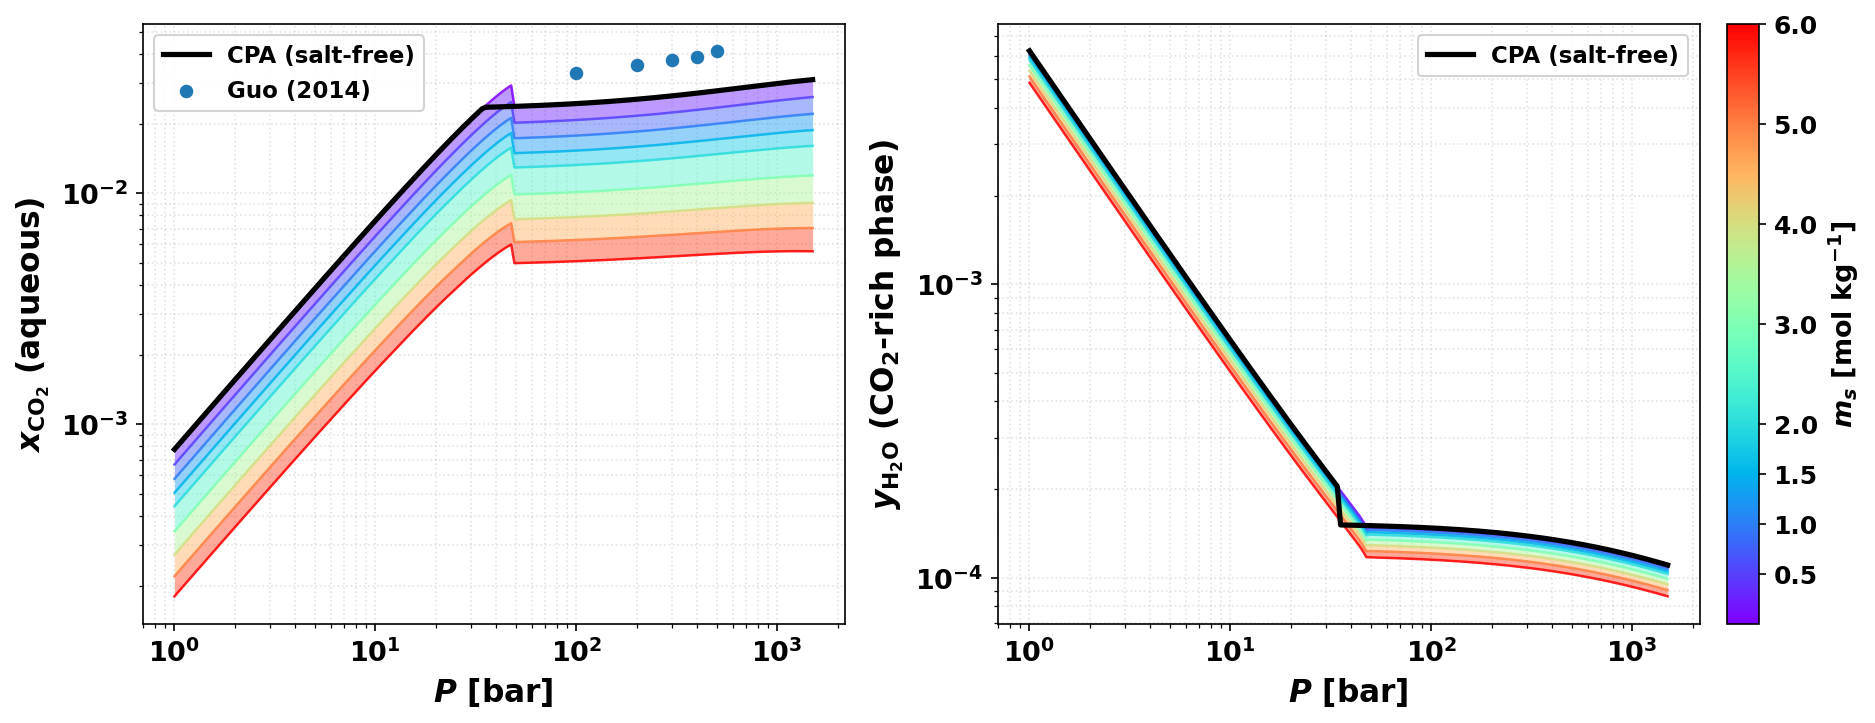
\includegraphics[width=\textwidth]{fig_S1a.png}\caption{$0\,^\circ$C\,(273\,K)}\end{subfigure}\\[6pt]
  \begin{subfigure}[t]{0.8\textwidth}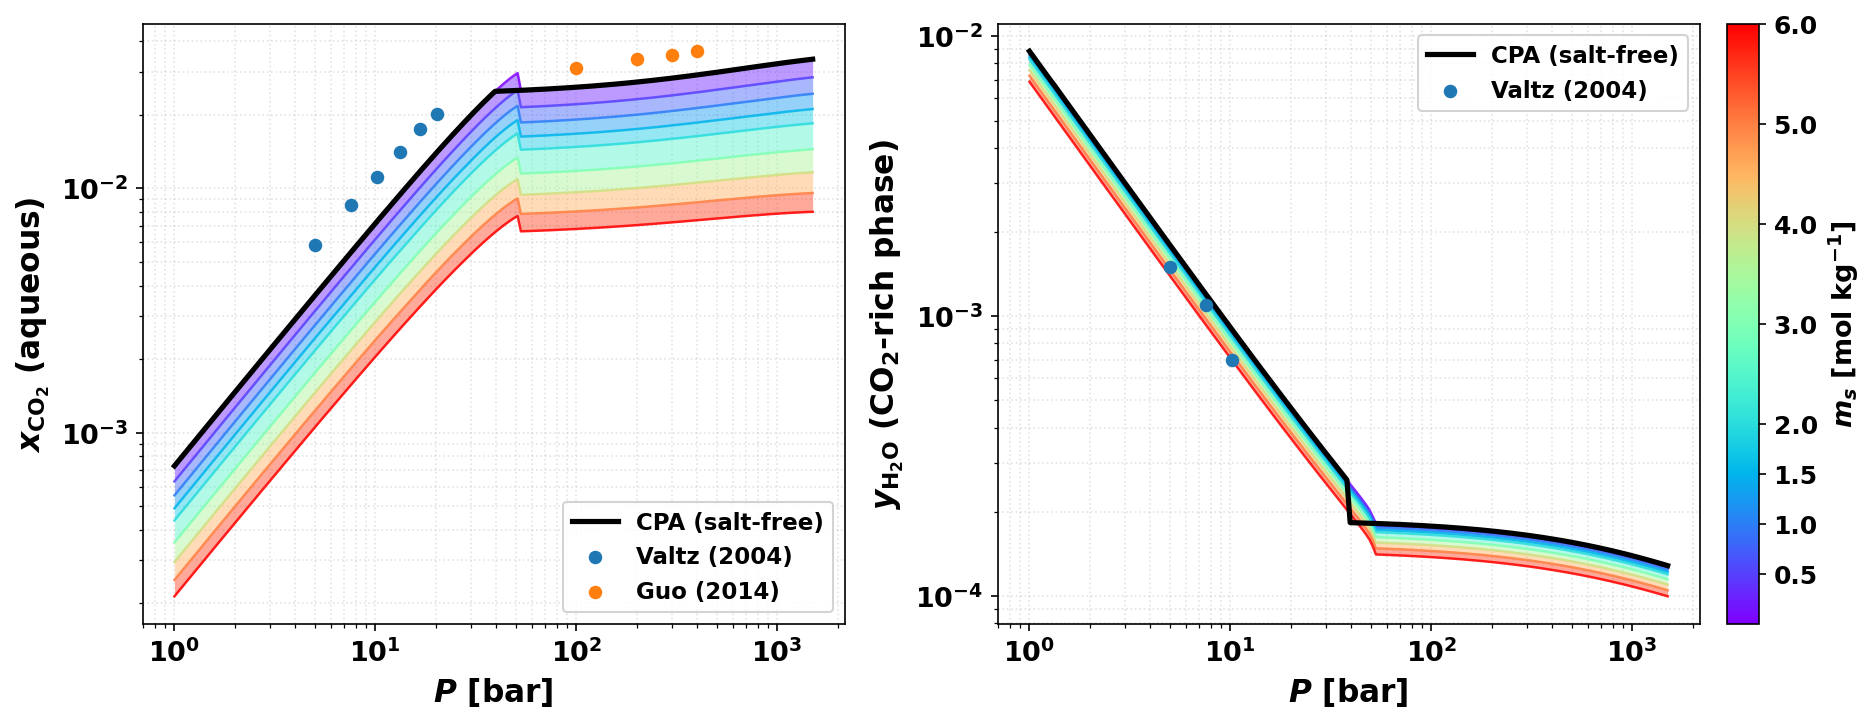
\includegraphics[width=\textwidth]{fig_S1b.png}\caption{$5\,^\circ$C\,(278\,K)}\end{subfigure}\\[6pt]
  \begin{subfigure}[t]{0.8\textwidth}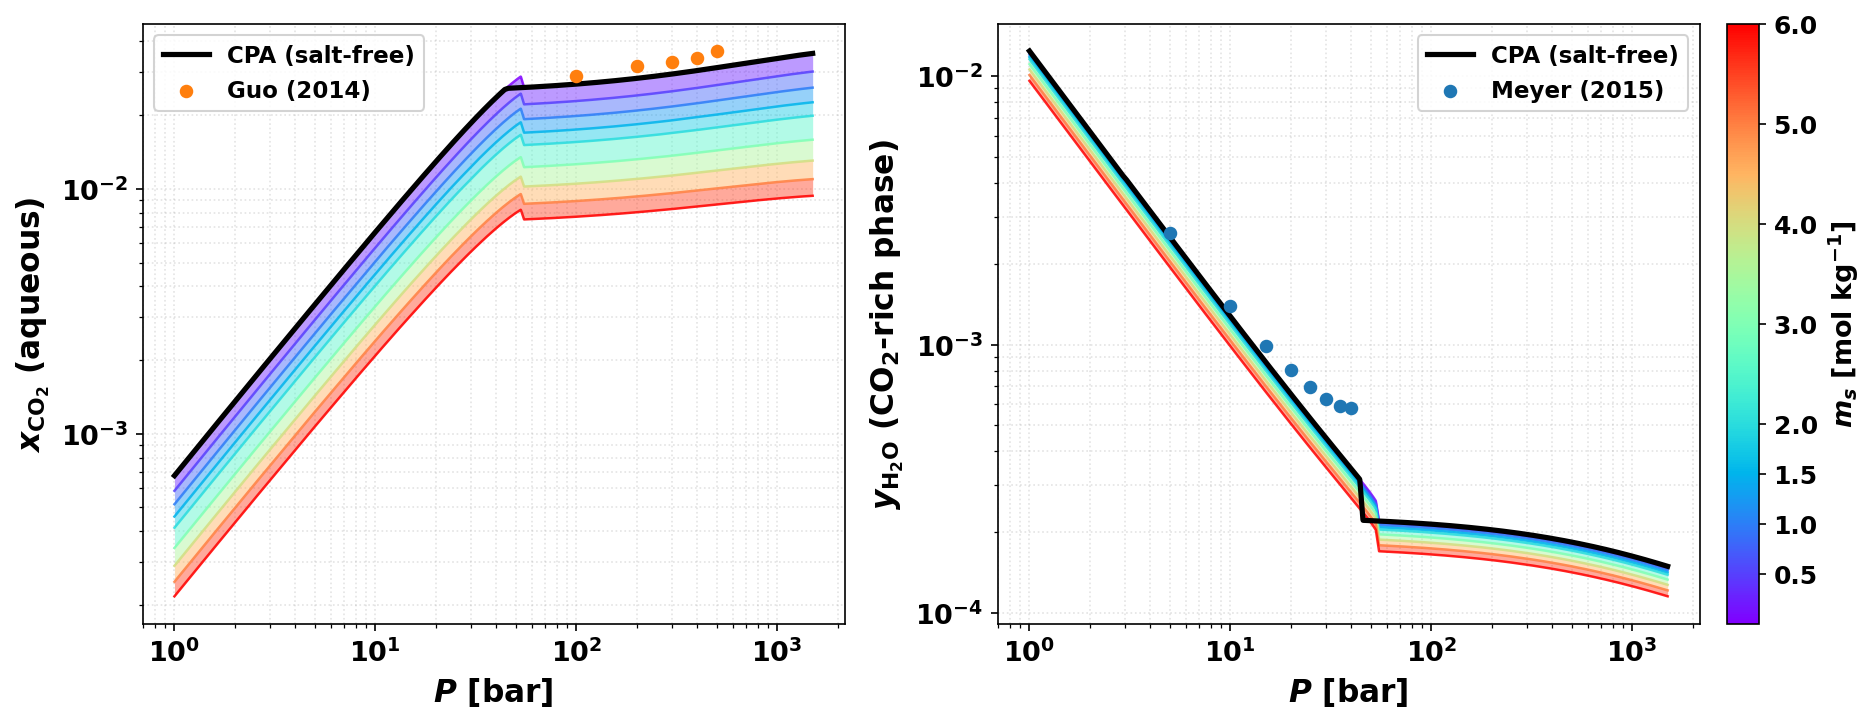
\includegraphics[width=\textwidth]{fig_S1c.png}\caption{$10\,^\circ$C\,(283\,K)}\end{subfigure}
  \caption{CO$_2$ + H$_2$O phase equilibria at all 32 temperatures not shown in
           Fig.~1 of the main text ($0$--$350\,^\circ$C), one temperature per row.
           For each temperature, we show the CO$_2$ mole fraction in the aqueous phase ($x_{\text{CO}_2}$,
           left panel) and H$_2$O mole fraction in the CO$_2$-rich phase
           ($y_{\text{H}_2\text{O}}$, right panel) vs.\ pressure.
           Open symbols: experimental data \citep{Coelho2025}; black solid line: CPA (salt-free);
           rainbow-colored filled bands: eCPA spanning $m_s = 0$--$6$\,mol\,kg$^{-1}$
           (violet to red), with discrete molality contours overlaid. This figure continues through the next pages.}
  \label{fig:co2h2o_Tpanel_SI}
\end{figure}

%% Page 2: 15–35°C
\begin{figure}[H]\ContinuedFloat
  \centering
  \begin{subfigure}[t]{0.8\textwidth}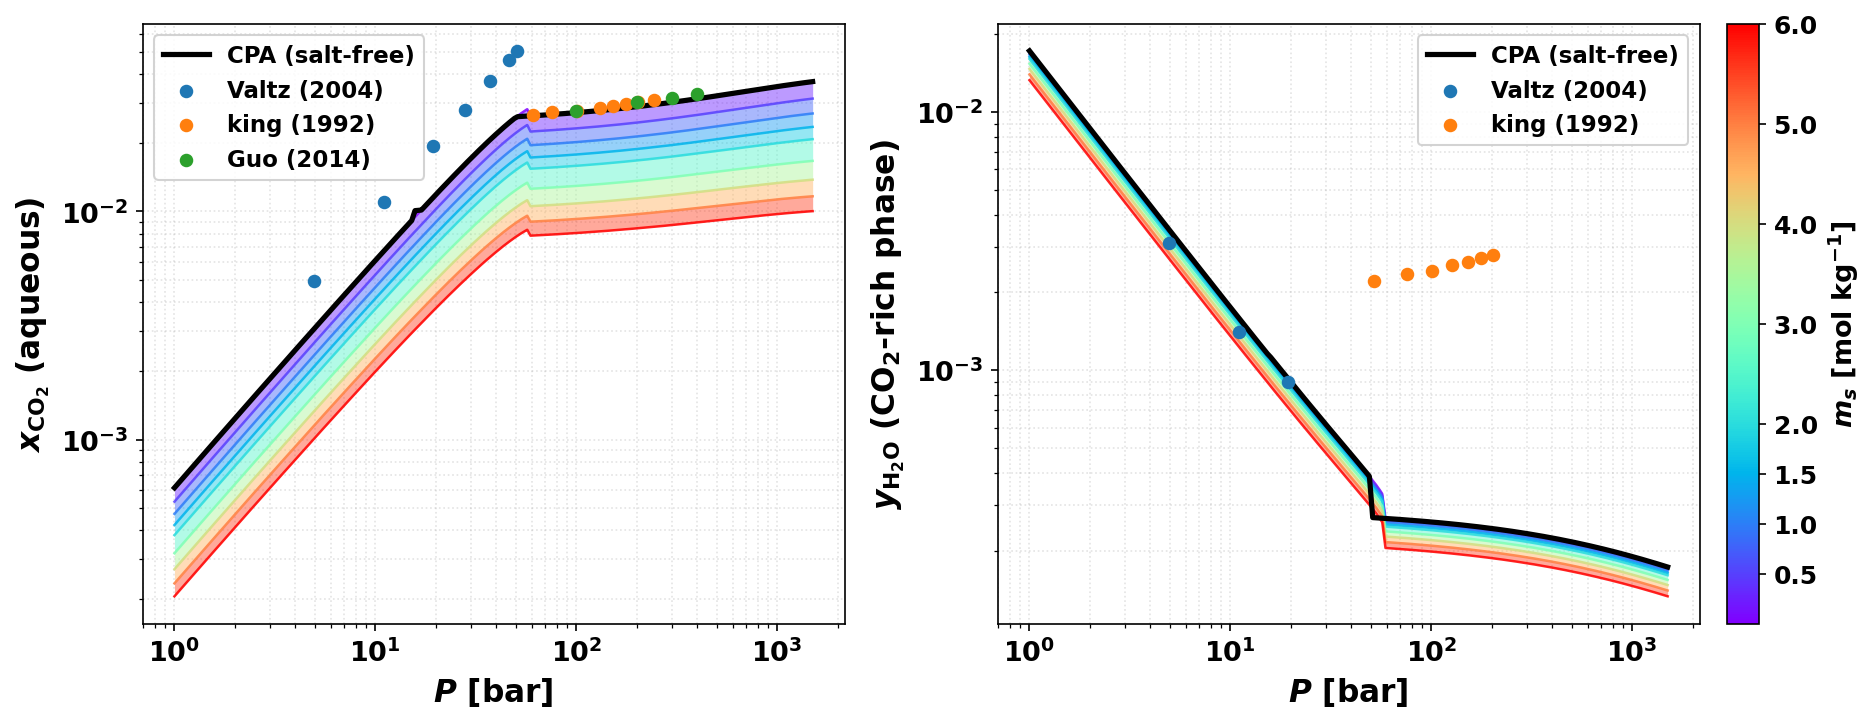
\includegraphics[width=\textwidth]{fig_S1d.png}\caption{$15\,^\circ$C\,(288\,K)}\end{subfigure}\\[6pt]
  \begin{subfigure}[t]{0.8\textwidth}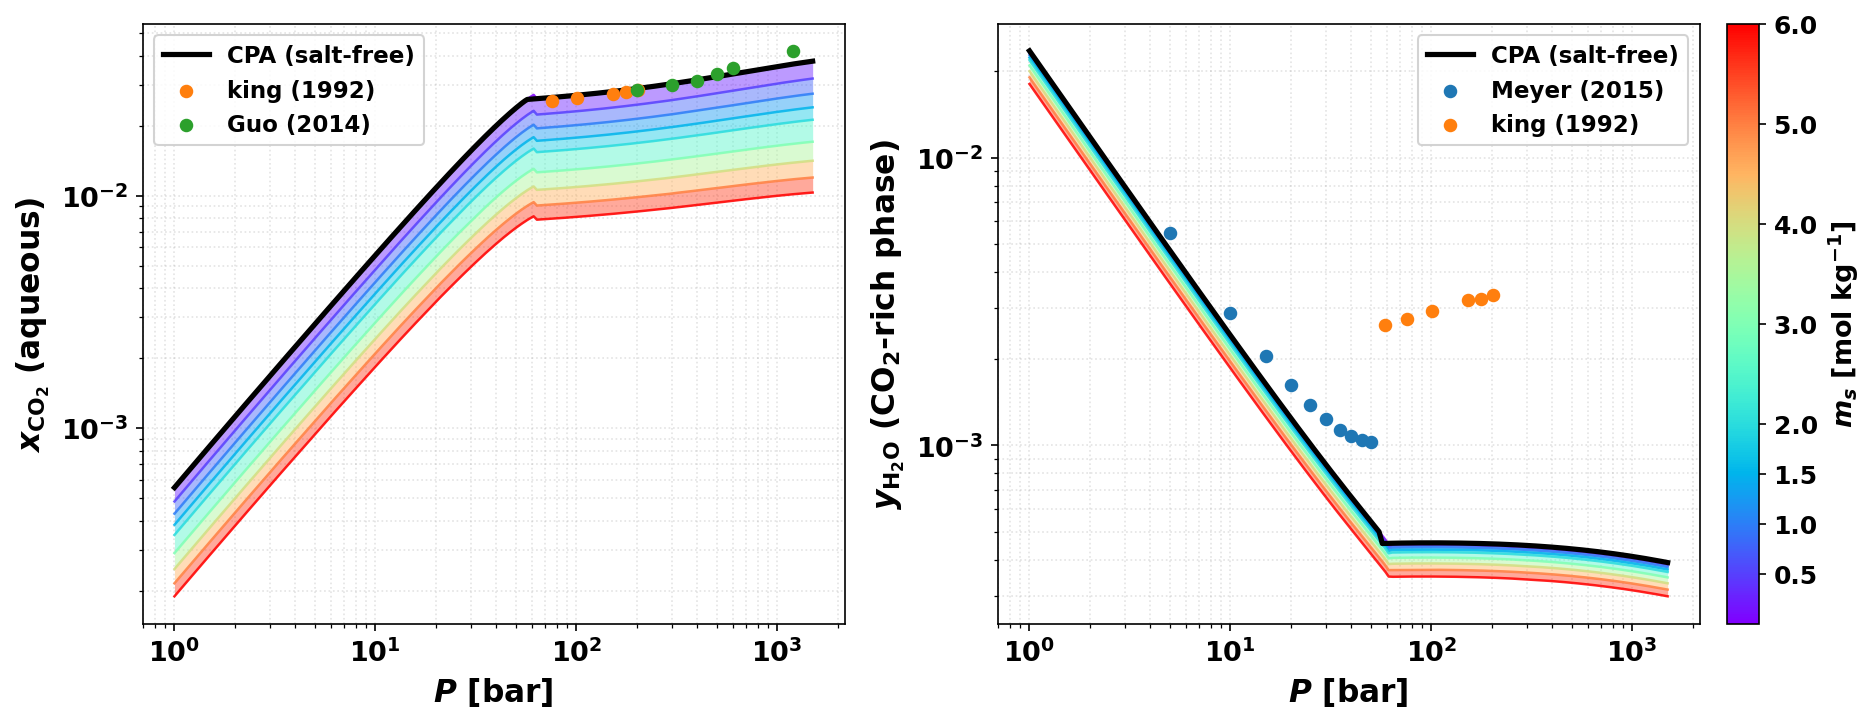
\includegraphics[width=\textwidth]{fig_S1e.png}\caption{$20\,^\circ$C\,(293\,K)}\end{subfigure}\\[6pt]
  \begin{subfigure}[t]{0.8\textwidth}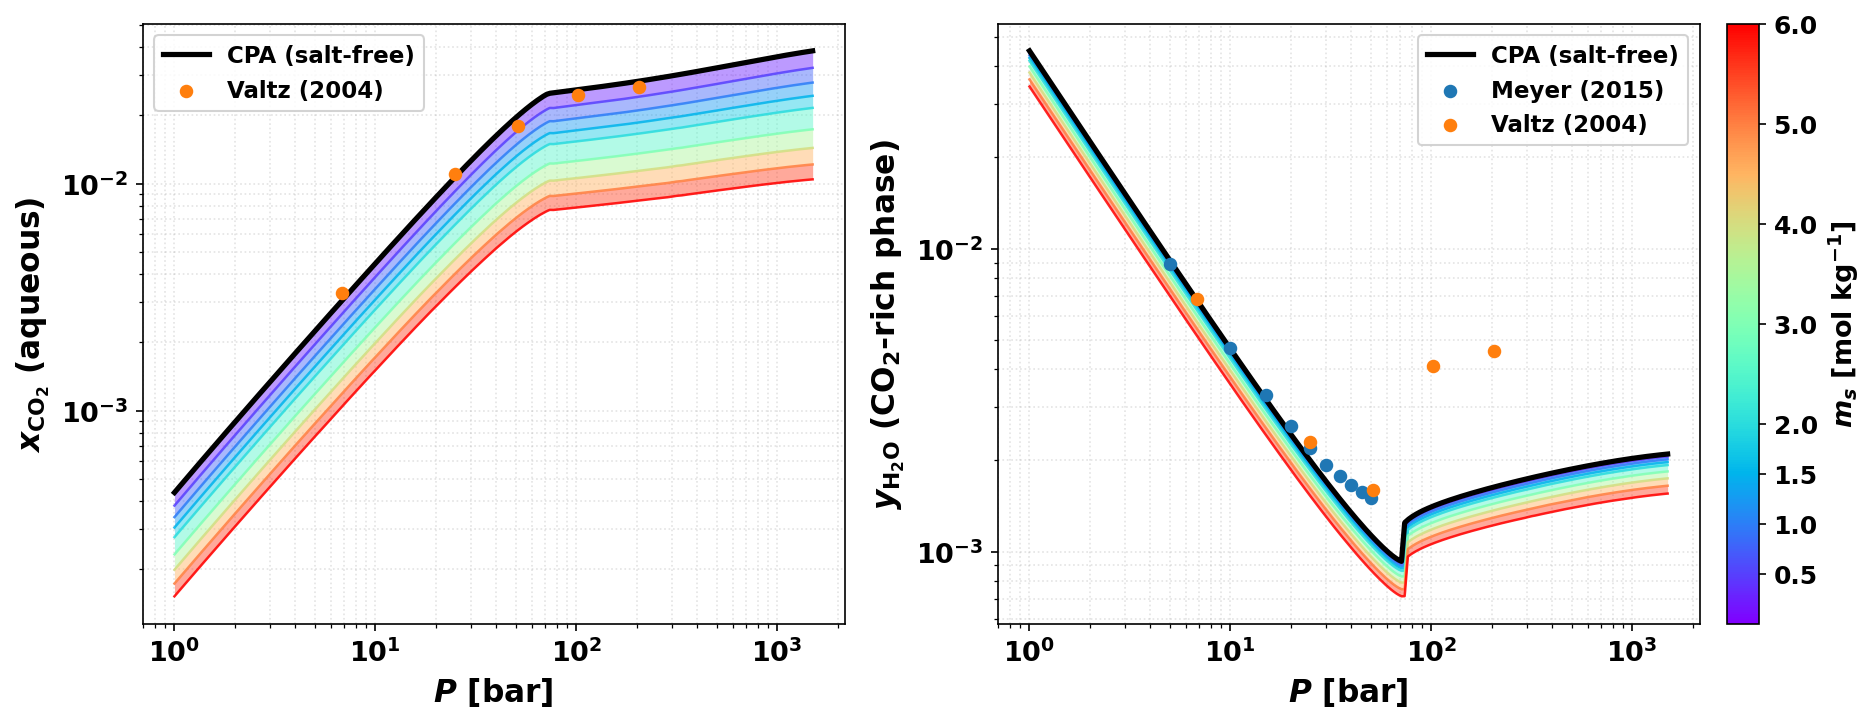
\includegraphics[width=\textwidth]{fig_S1f.png}\caption{$31\,^\circ$C\,(304\,K)}\end{subfigure}
  \caption{(\emph{continued})}
\end{figure}

%% Page 3: 35–45°C
\begin{figure}[H]\ContinuedFloat
  \centering
  \begin{subfigure}[t]{0.8\textwidth}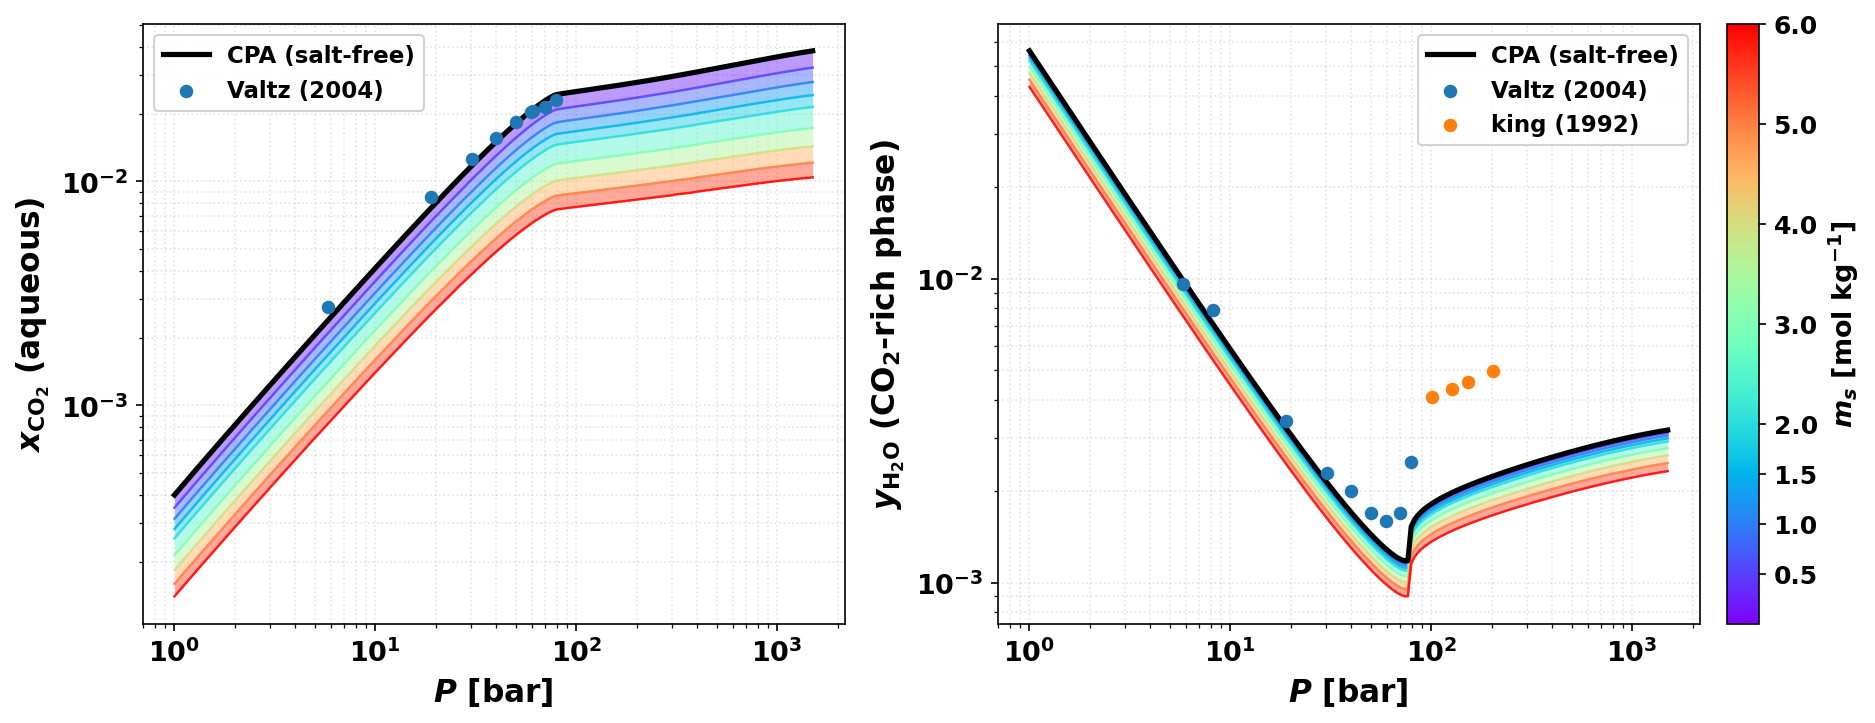
\includegraphics[width=\textwidth]{fig_S1g.png}\caption{$35\,^\circ$C\,(308\,K)}\end{subfigure}\\[6pt]
  \begin{subfigure}[t]{0.8\textwidth}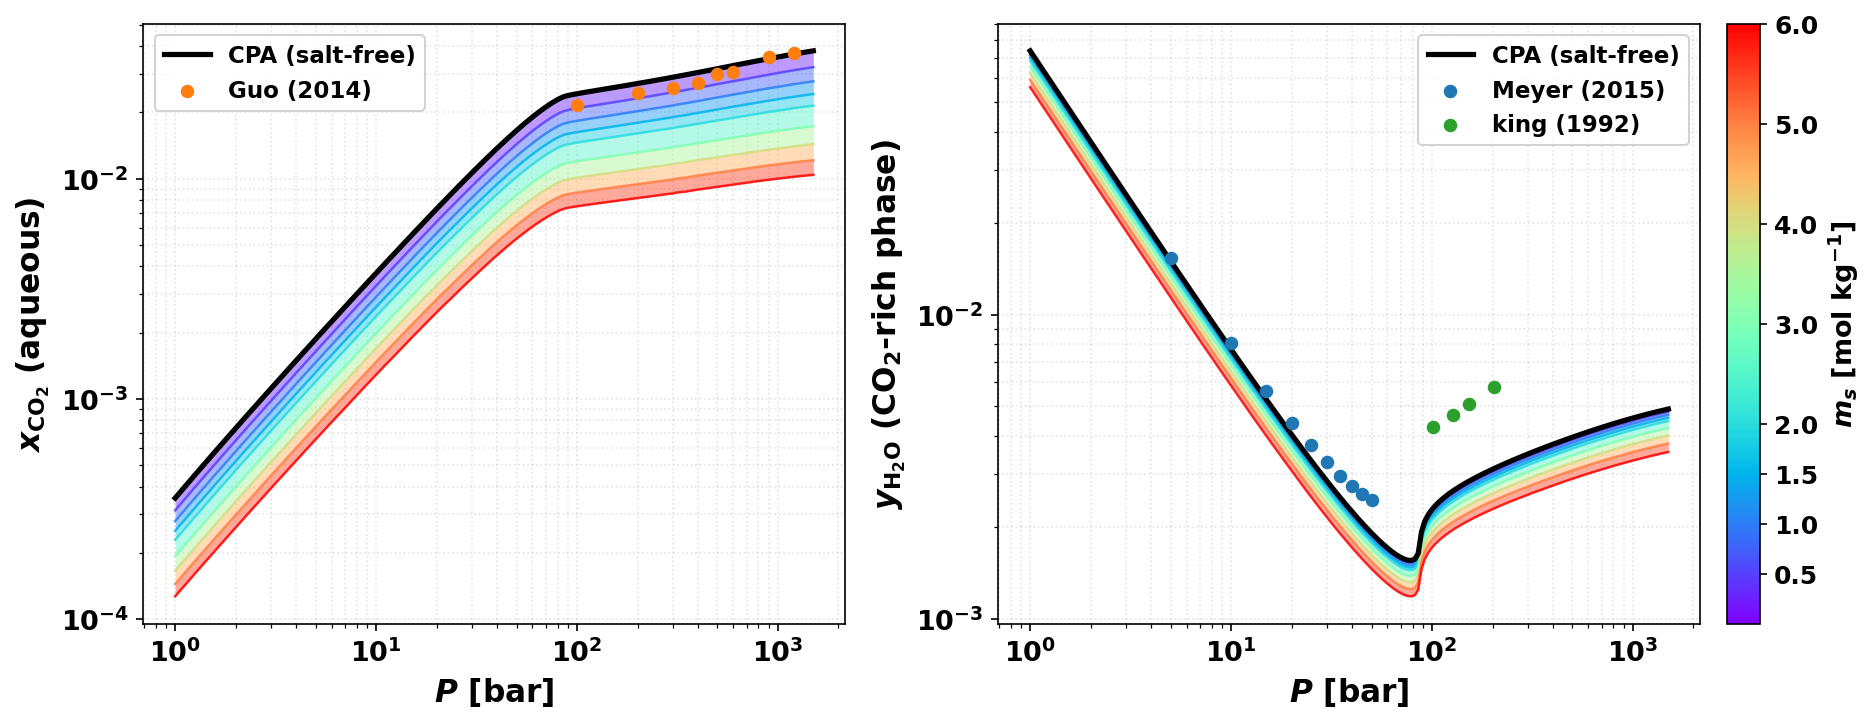
\includegraphics[width=\textwidth]{fig_S1h.png}\caption{$40\,^\circ$C\,(313\,K)}\end{subfigure}\\[6pt]
  \begin{subfigure}[t]{0.8\textwidth}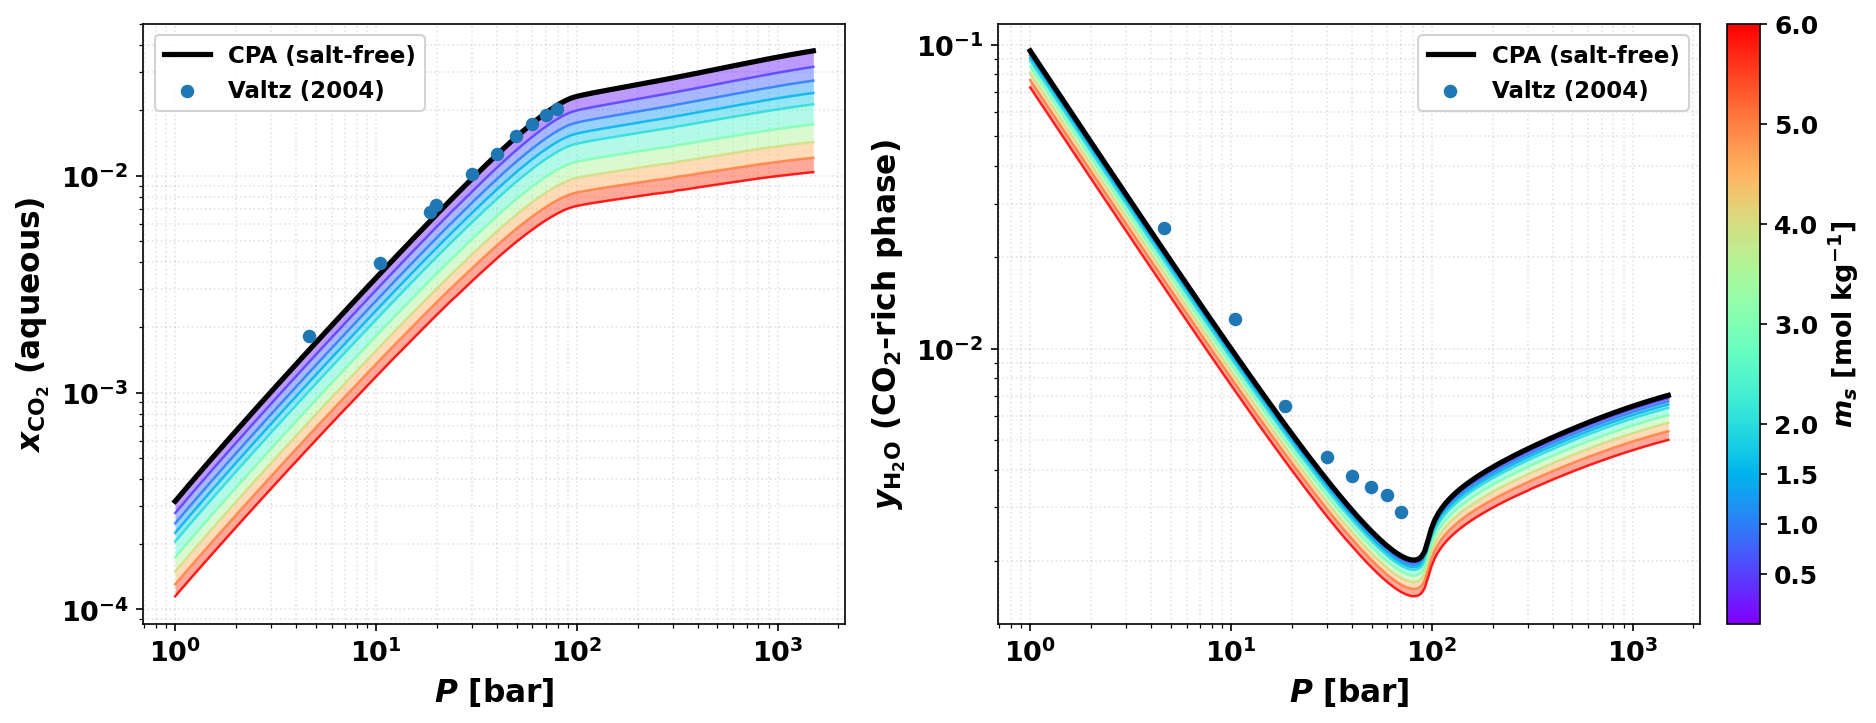
\includegraphics[width=\textwidth]{fig_S1i.png}\caption{$45\,^\circ$C\,(318\,K)}\end{subfigure}
  \caption{(\emph{continued})}
\end{figure}

%% Page 4: 50–75°C (50°C from main Fig.~1)
\begin{figure}[H]\ContinuedFloat
  \centering
  \begin{subfigure}[t]{0.8\textwidth}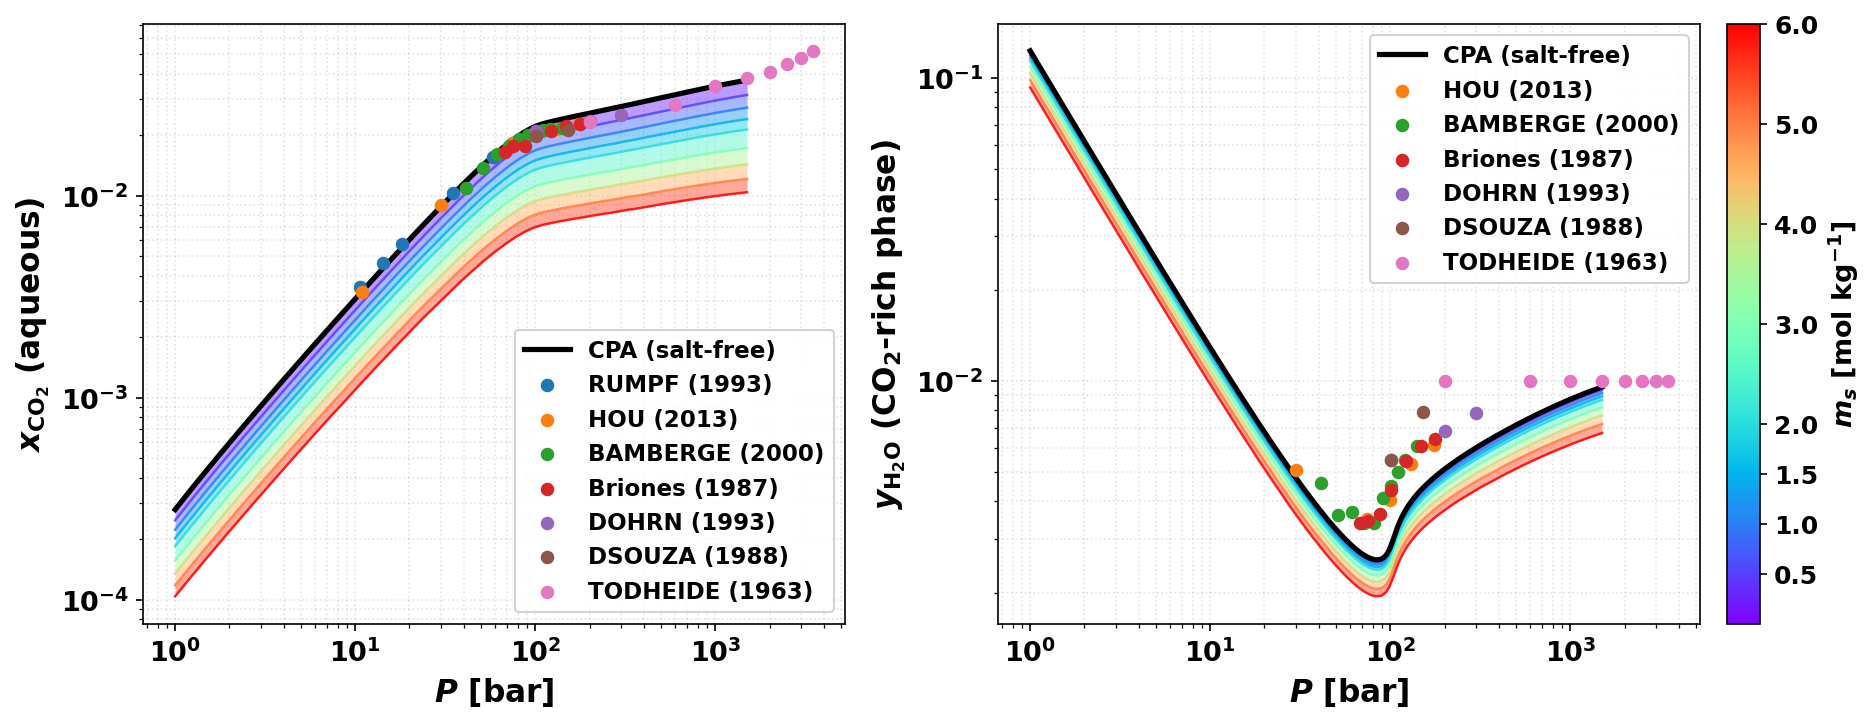
\includegraphics[width=\textwidth]{fig_1b.png}\caption{$50\,^\circ$C\,(323\,K)}\end{subfigure}\\[6pt]
  \begin{subfigure}[t]{0.8\textwidth}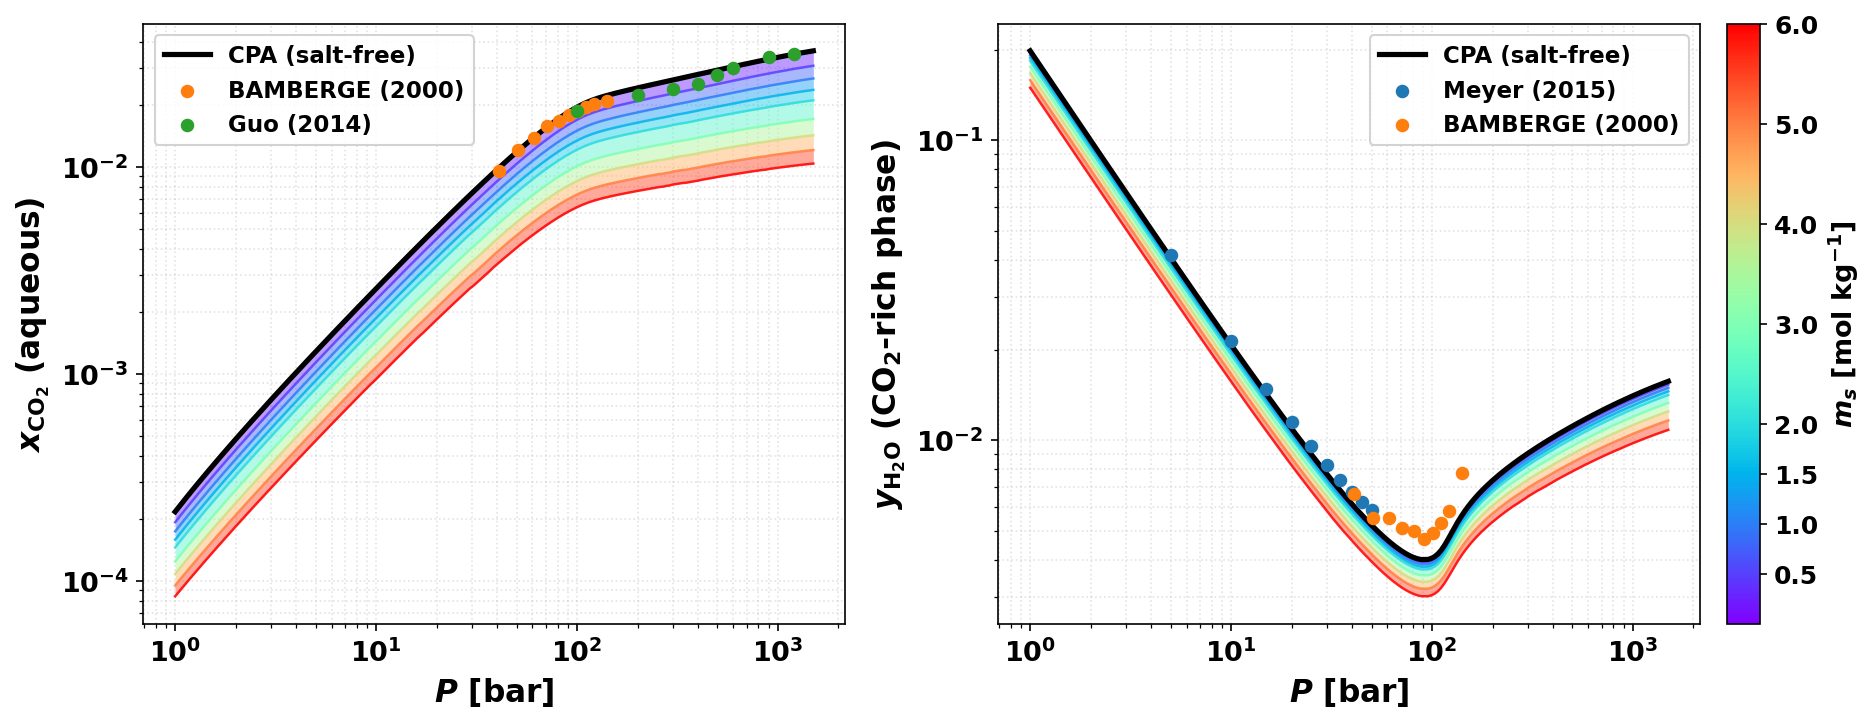
\includegraphics[width=\textwidth]{fig_S1j.png}\caption{$60\,^\circ$C\,(333\,K)}\end{subfigure}\\[6pt]
  \begin{subfigure}[t]{0.8\textwidth}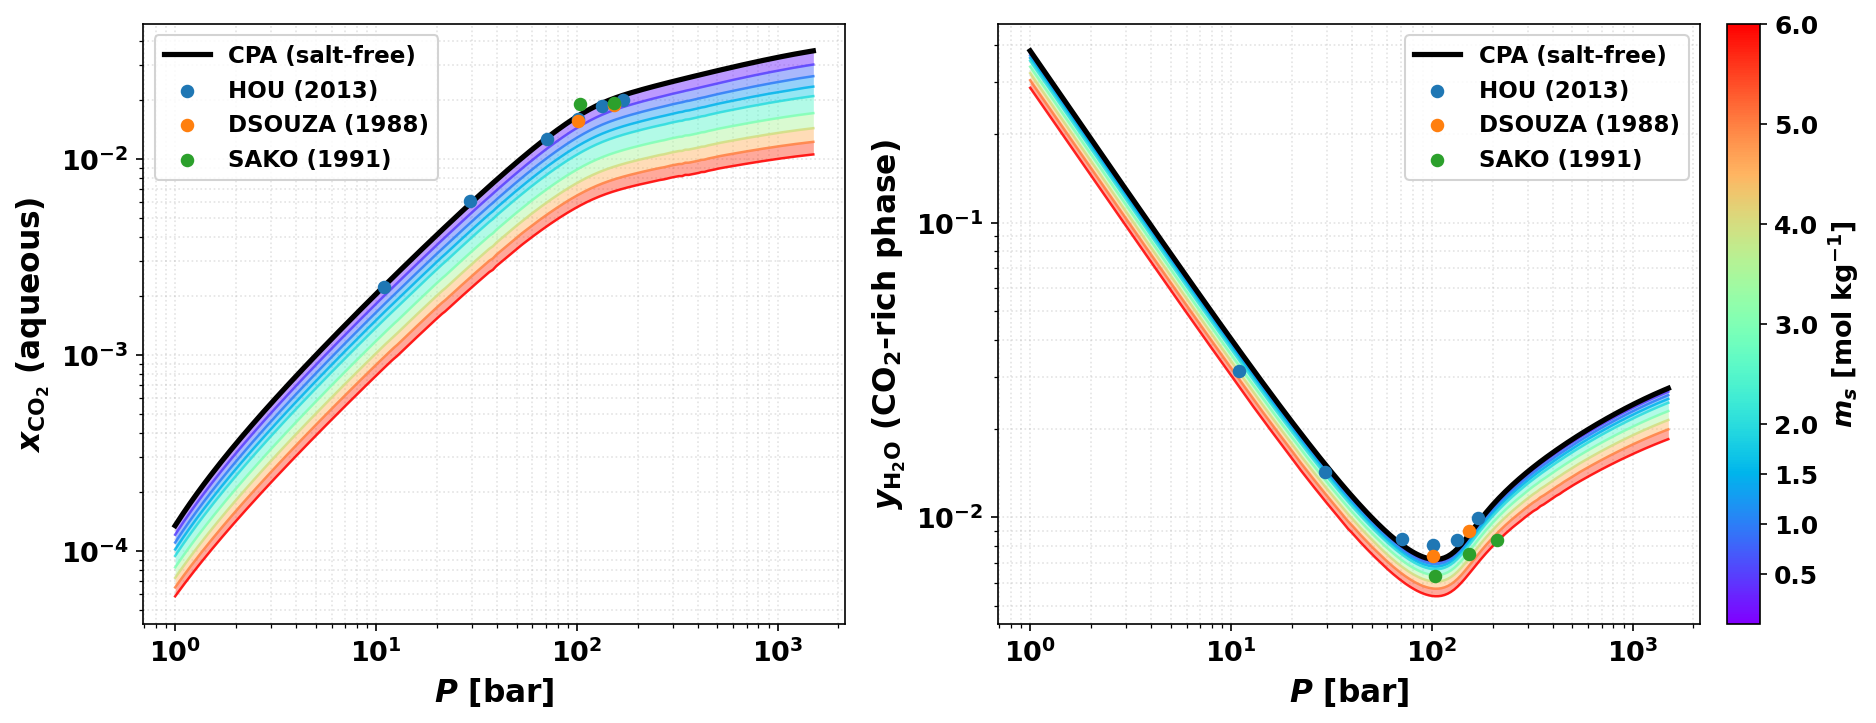
\includegraphics[width=\textwidth]{fig_S1k.png}\caption{$75\,^\circ$C\,(348\,K)}\end{subfigure}
  \caption{(\emph{continued})}
\end{figure}

%% Page 5: 80–110°C (100°C from main Fig.~1)
\begin{figure}[H]\ContinuedFloat
  \centering
  \begin{subfigure}[t]{0.8\textwidth}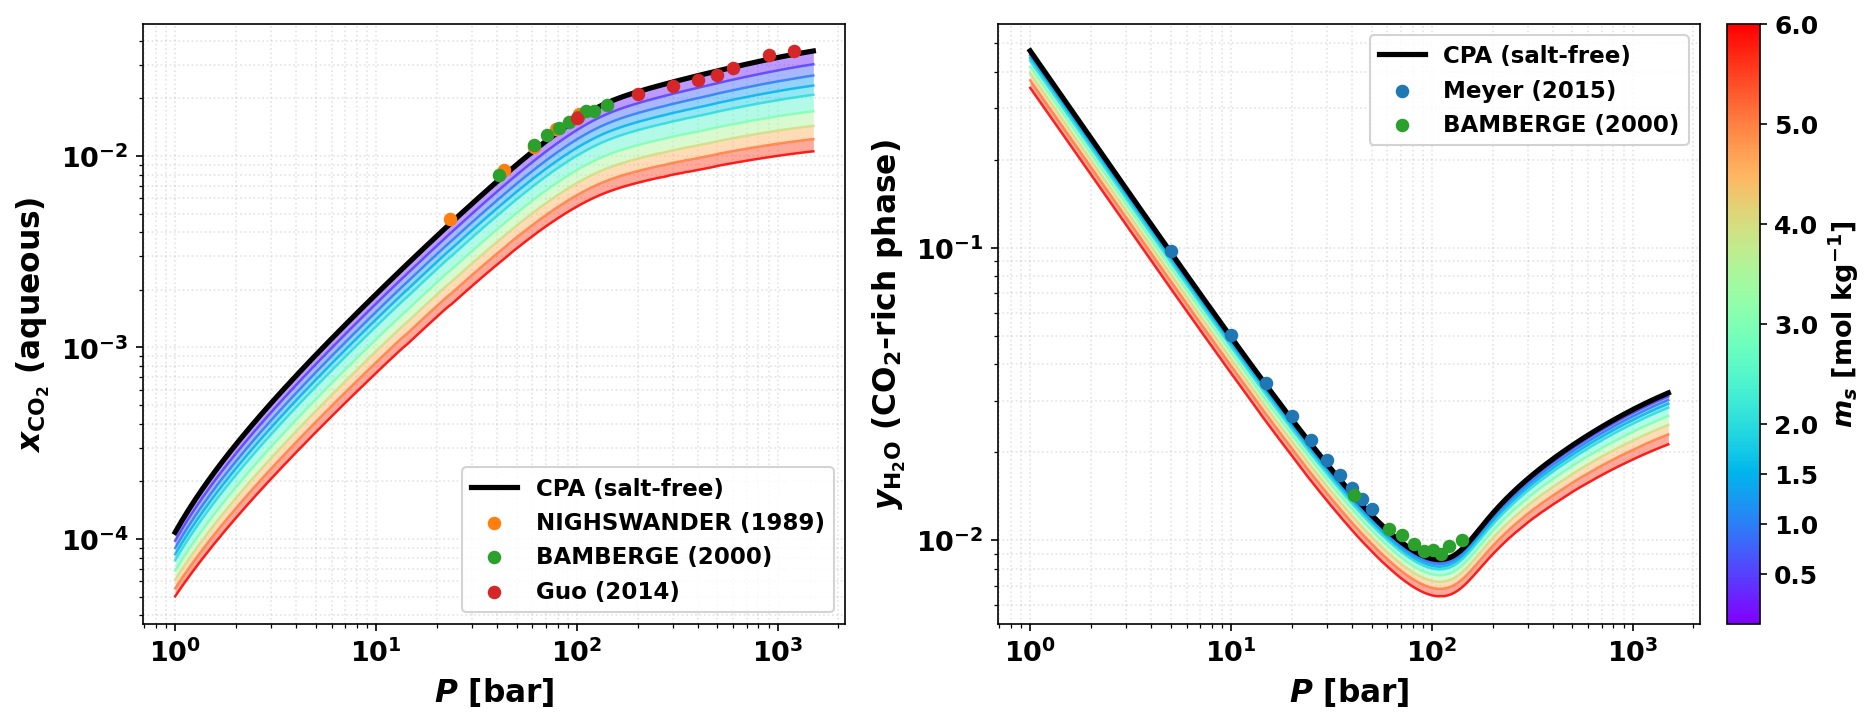
\includegraphics[width=\textwidth]{fig_S1l.png}\caption{$80\,^\circ$C\,(353\,K)}\end{subfigure}\\[6pt]
  \begin{subfigure}[t]{0.8\textwidth}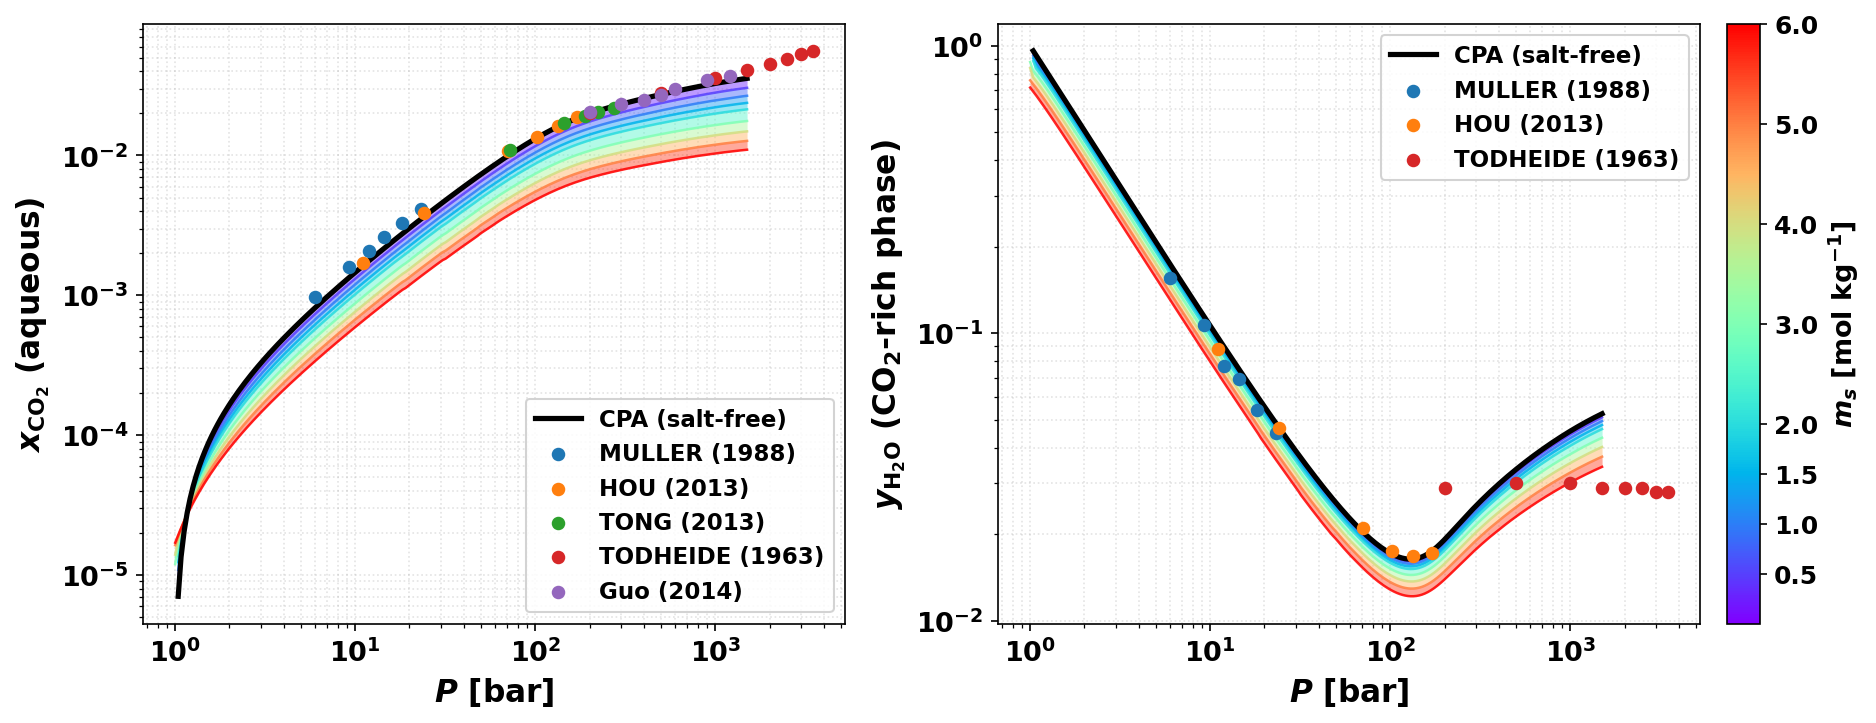
\includegraphics[width=\textwidth]{fig_1c.png}\caption{$100\,^\circ$C\,(373\,K)}\end{subfigure}\\[6pt]
  \begin{subfigure}[t]{0.8\textwidth}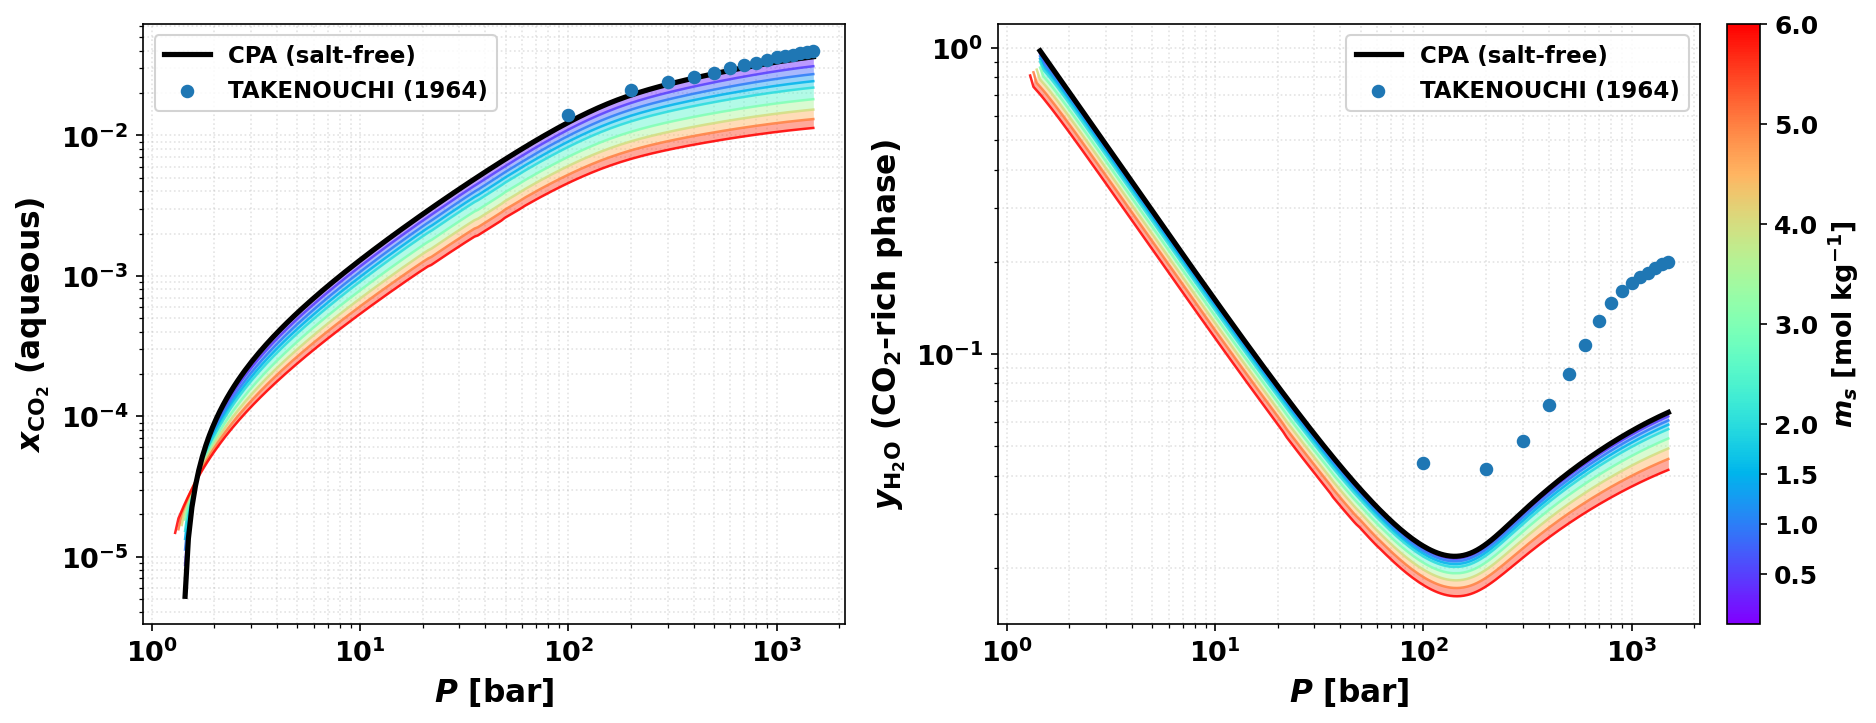
\includegraphics[width=\textwidth]{fig_S1m.png}\caption{$110\,^\circ$C\,(383\,K)}\end{subfigure}
  \caption{(\emph{continued})}
\end{figure}

%% Page 6: 120–160°C
\begin{figure}[H]\ContinuedFloat
  \centering
  \begin{subfigure}[t]{0.8\textwidth}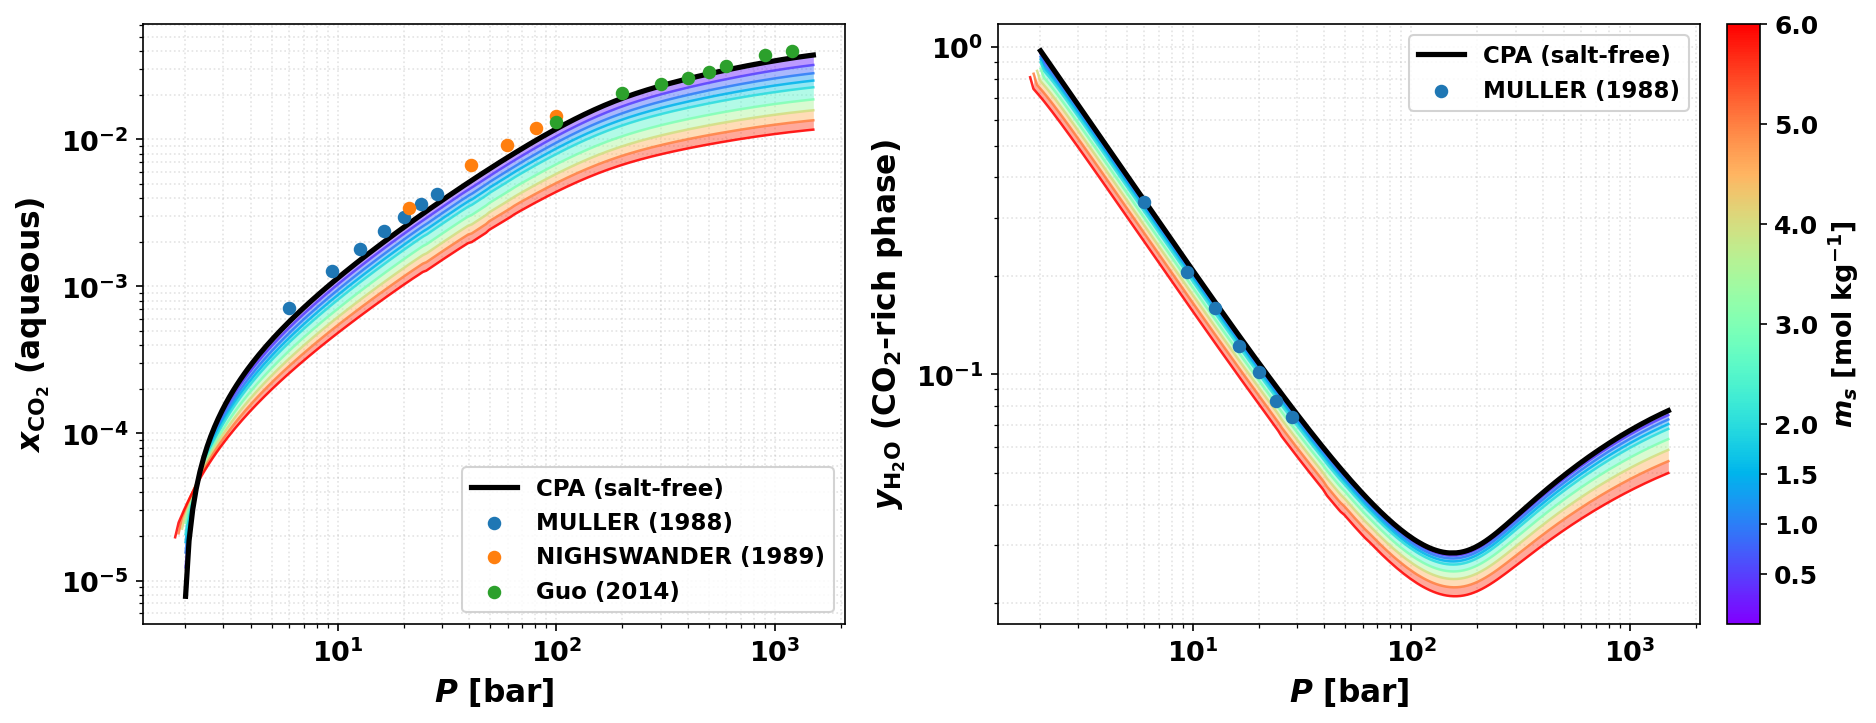
\includegraphics[width=\textwidth]{fig_S1n.png}\caption{$120\,^\circ$C\,(393\,K)}\end{subfigure}\\[6pt]
  \begin{subfigure}[t]{0.8\textwidth}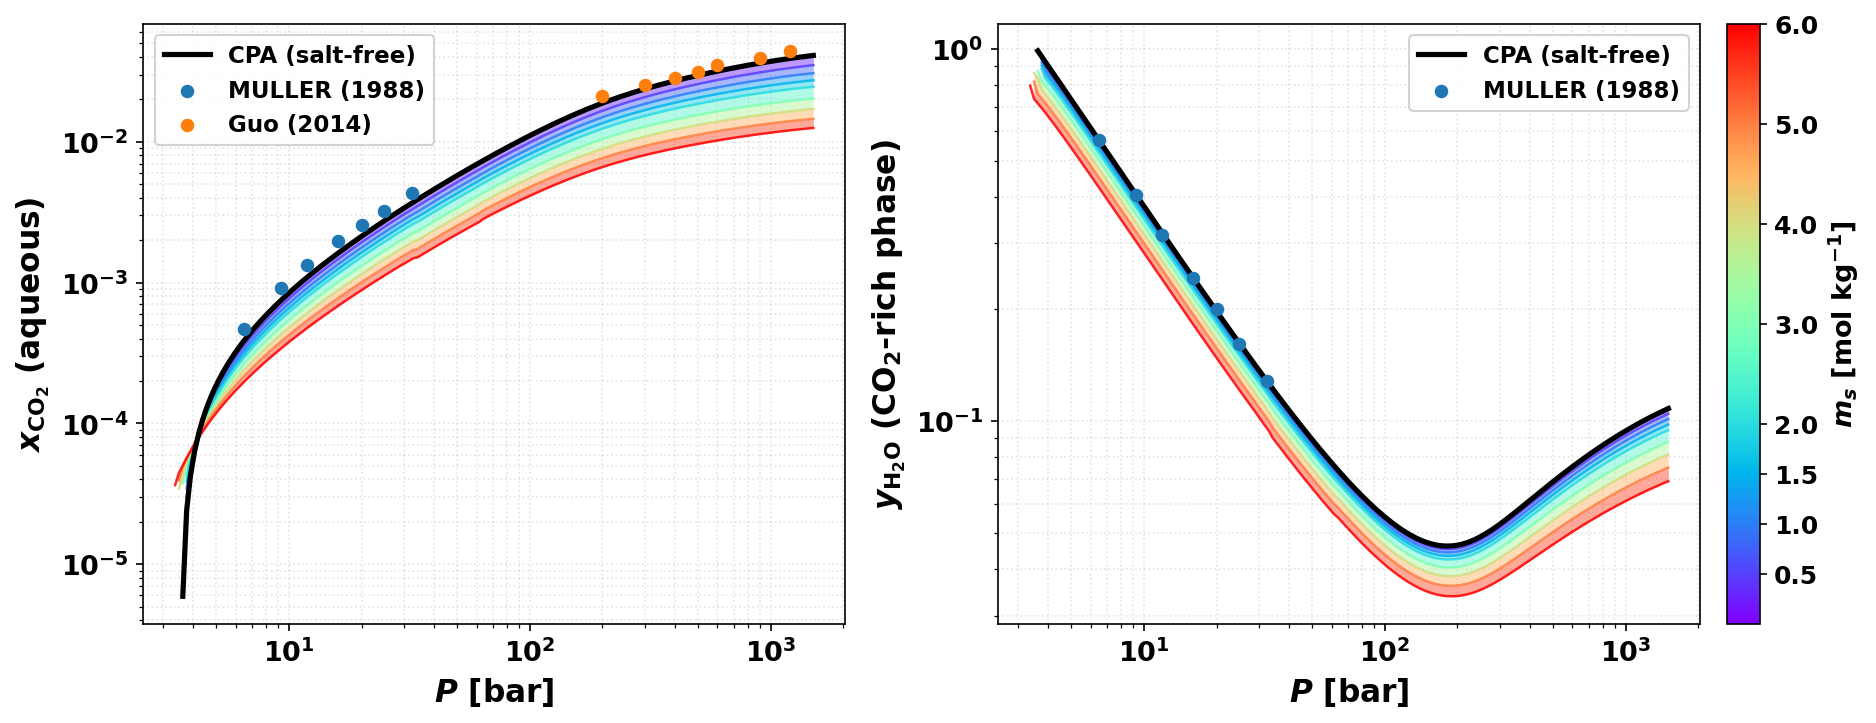
\includegraphics[width=\textwidth]{fig_S1o.png}\caption{$140\,^\circ$C\,(413\,K)}\end{subfigure}\\[6pt]
  \begin{subfigure}[t]{0.8\textwidth}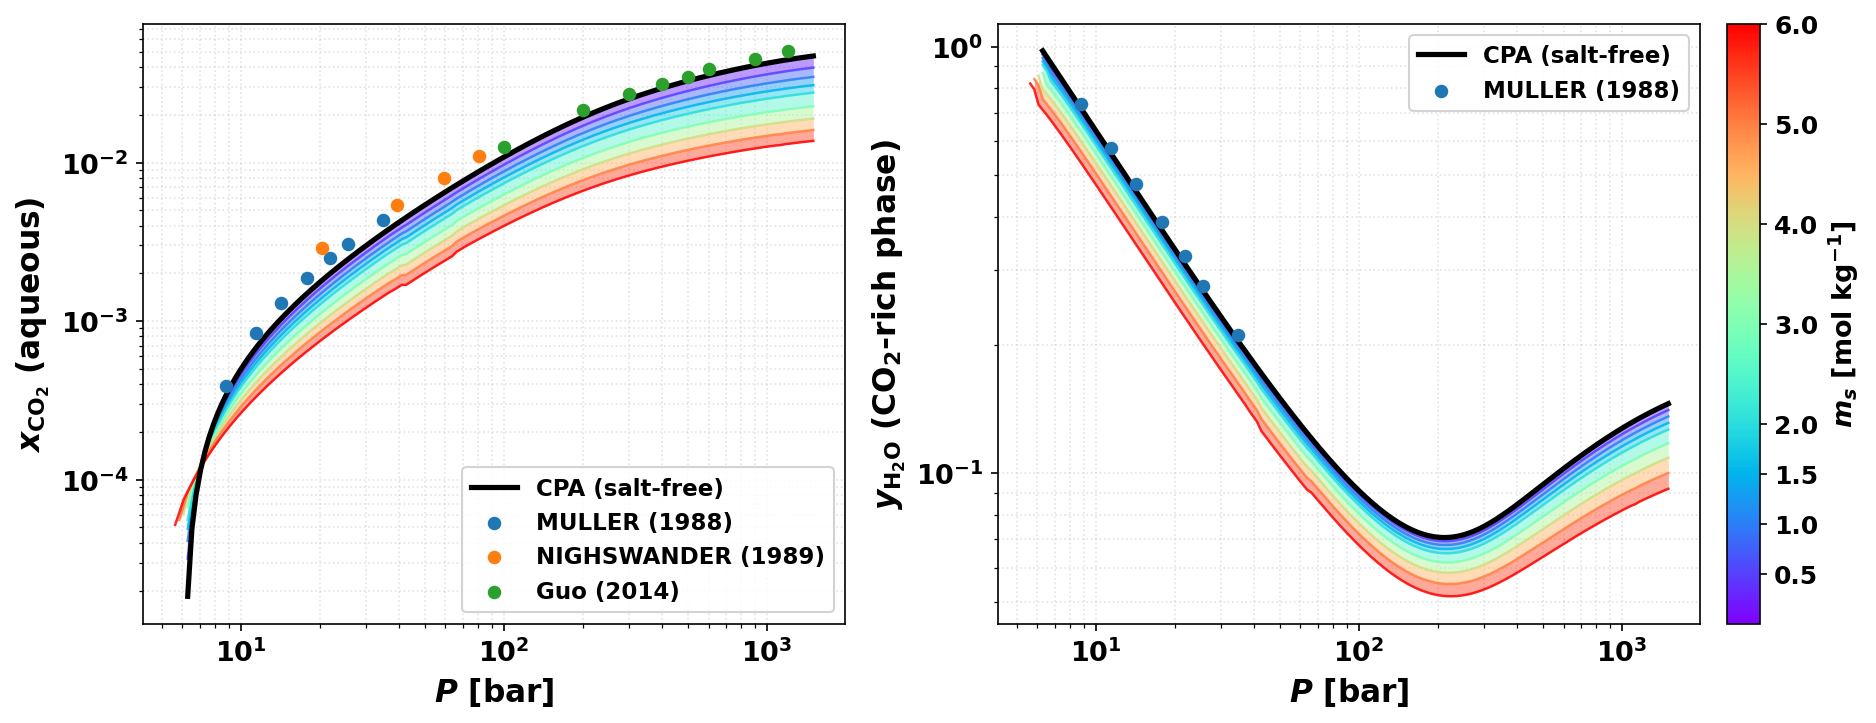
\includegraphics[width=\textwidth]{fig_S1p.png}\caption{$160\,^\circ$C\,(433\,K)}\end{subfigure}
  \caption{(\emph{continued})}
\end{figure}

%% Page 7: 175–200°C (200°C from main Fig.~1)
\begin{figure}[H]\ContinuedFloat
  \centering
  \begin{subfigure}[t]{0.8\textwidth}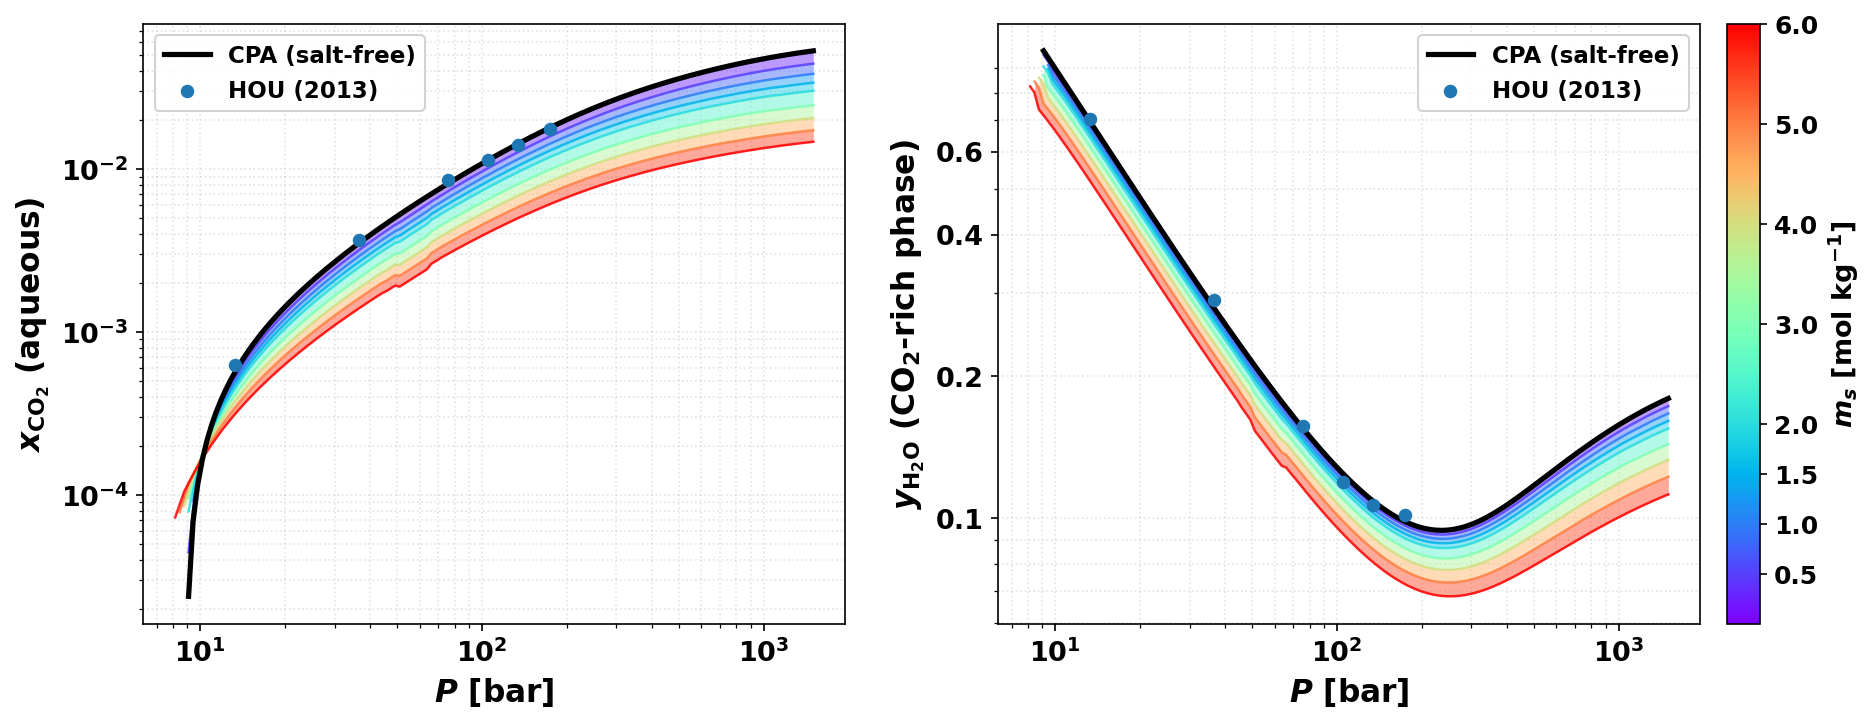
\includegraphics[width=\textwidth]{fig_S1q.png}\caption{$175\,^\circ$C\,(448\,K)}\end{subfigure}\\[6pt]
  \begin{subfigure}[t]{0.8\textwidth}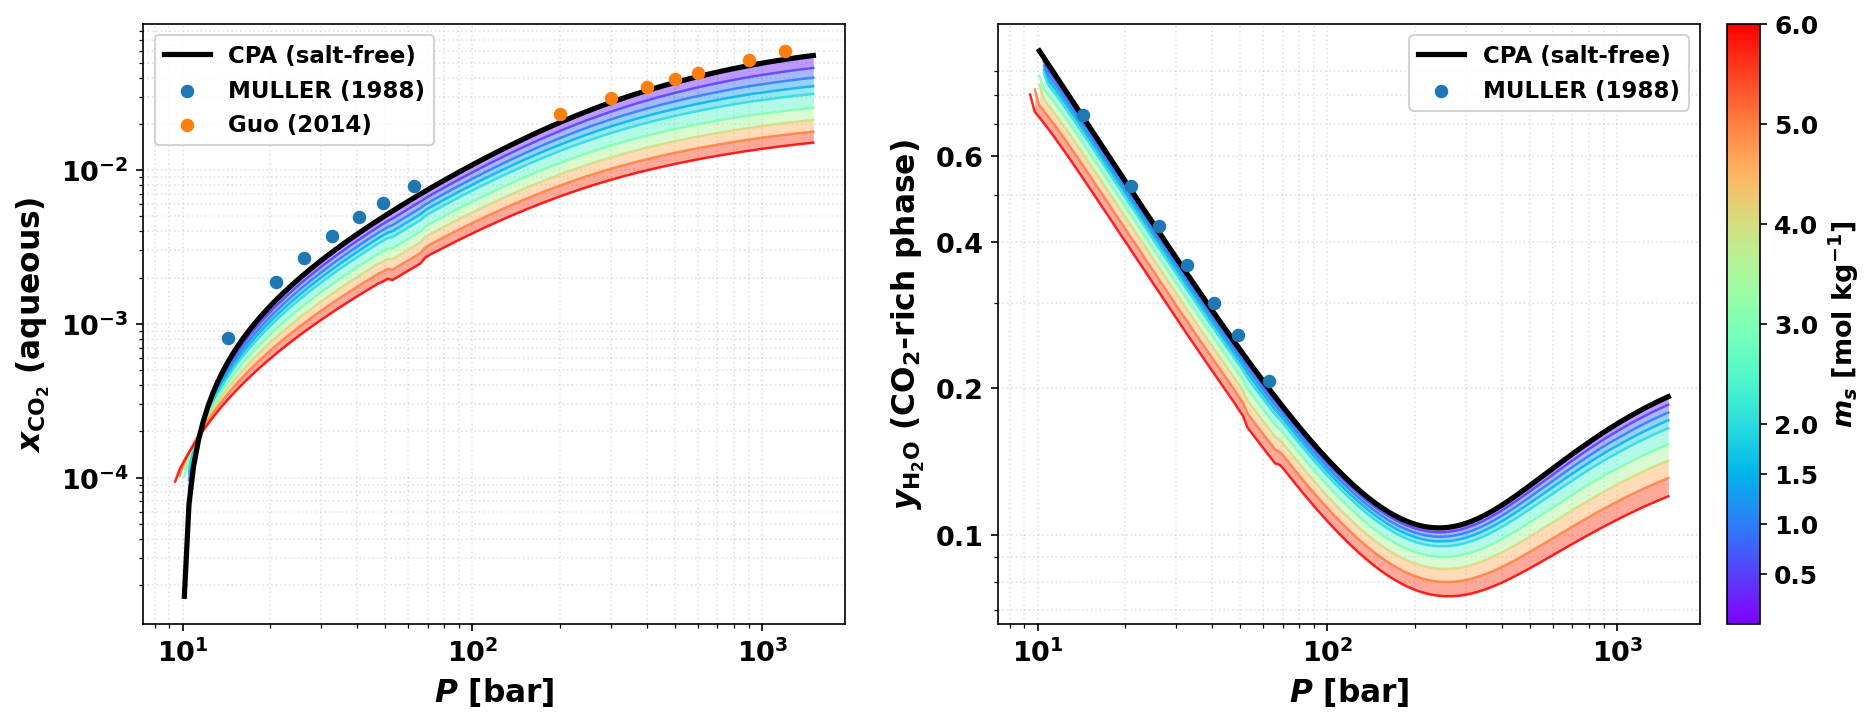
\includegraphics[width=\textwidth]{fig_S1r.png}\caption{$180\,^\circ$C\,(453\,K)}\end{subfigure}\\[6pt]
  \begin{subfigure}[t]{0.8\textwidth}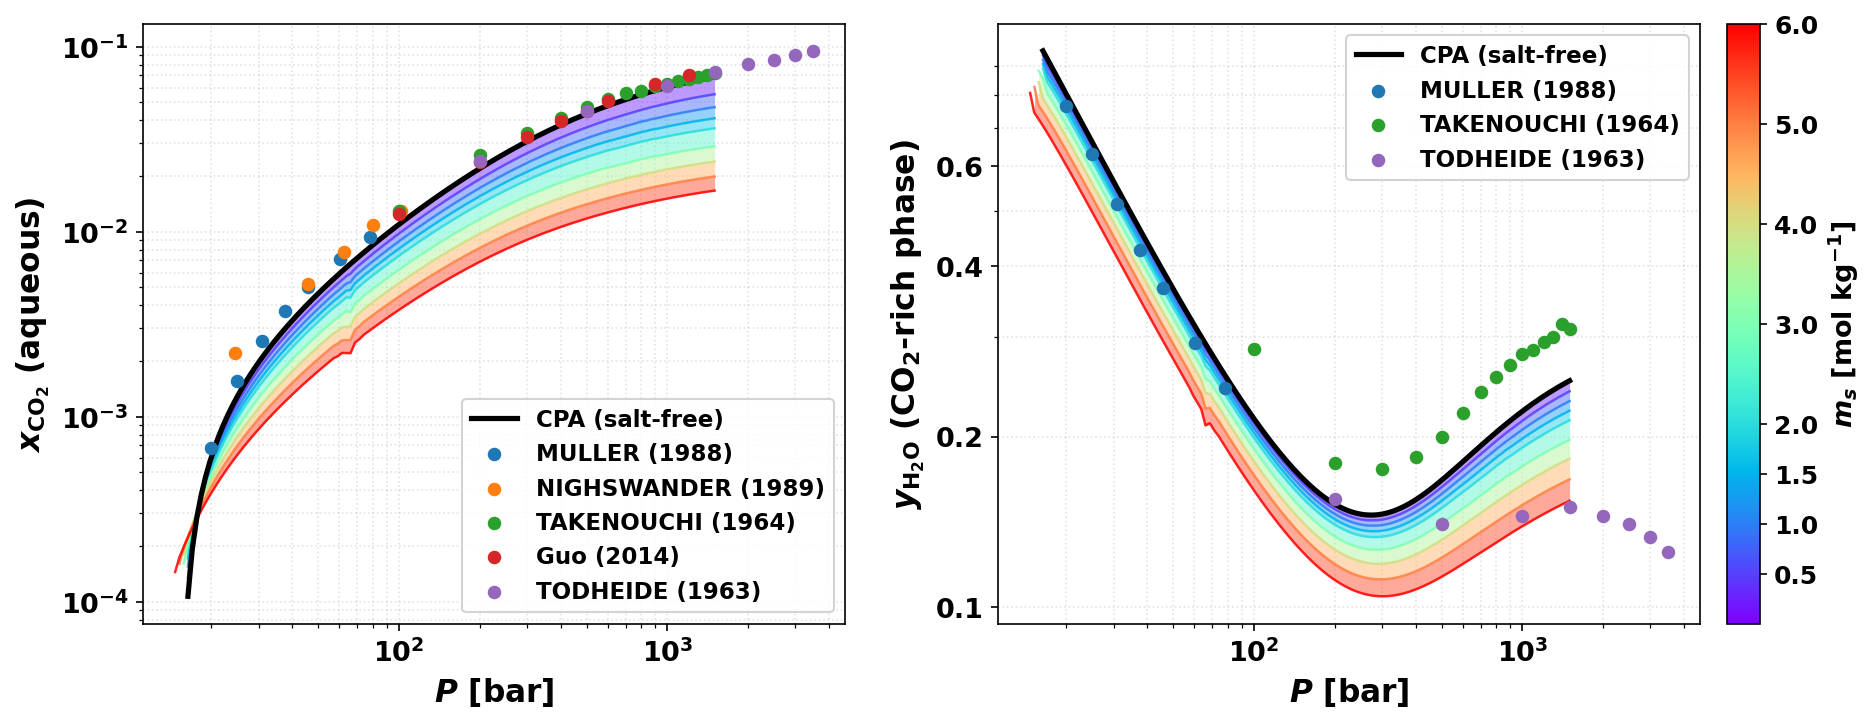
\includegraphics[width=\textwidth]{fig_1e.png}\caption{$200\,^\circ$C\,(473\,K)}\end{subfigure}
  \caption{(\emph{continued})}
\end{figure}

%% Page 8: 220–260°C
\begin{figure}[H]\ContinuedFloat
  \centering
  \begin{subfigure}[t]{0.8\textwidth}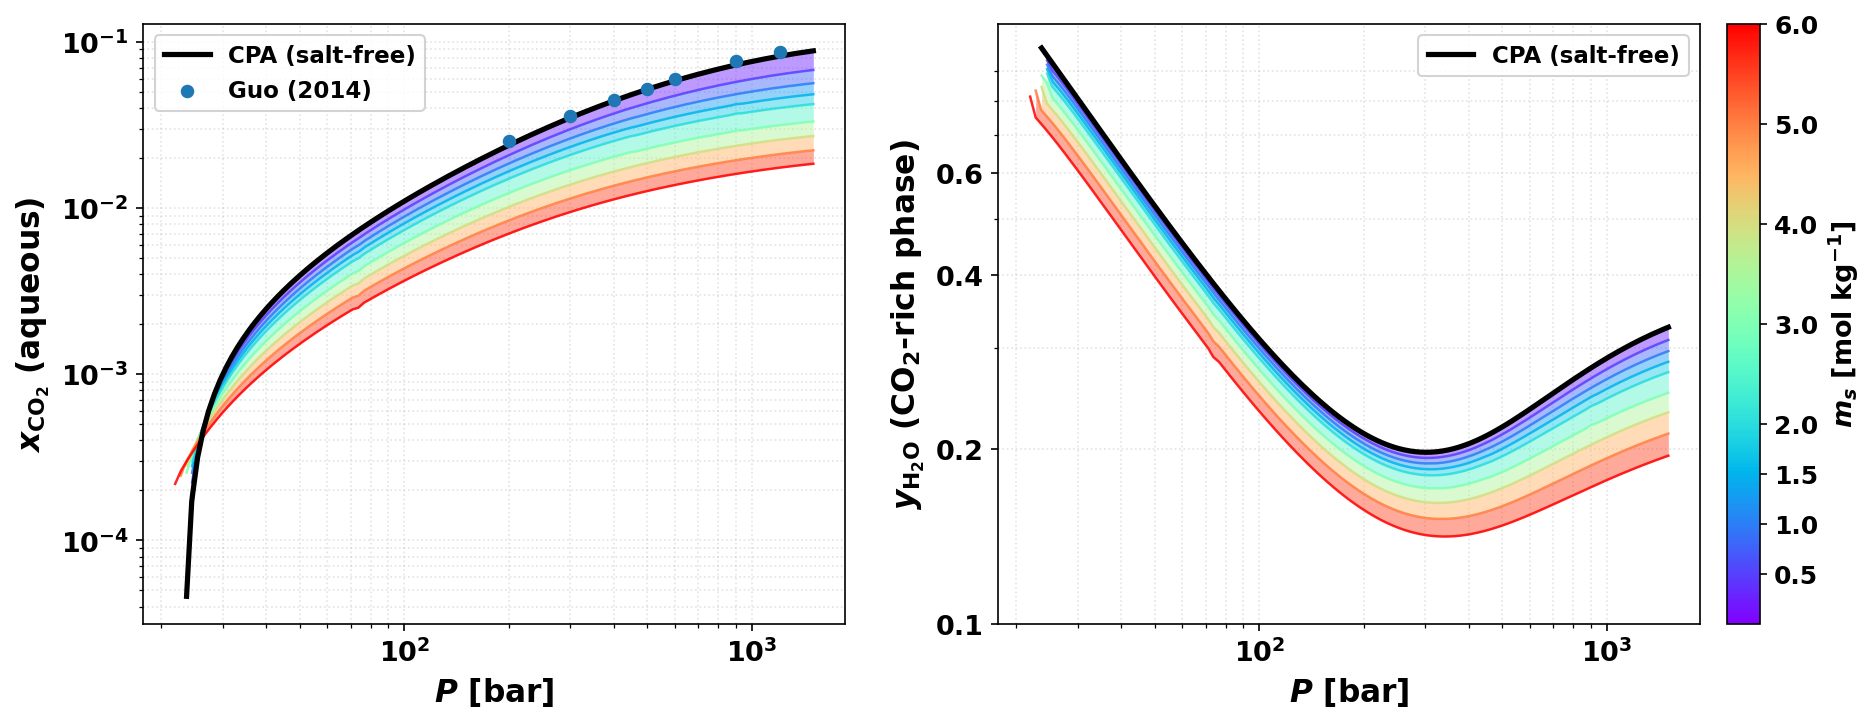
\includegraphics[width=\textwidth]{fig_S1s.png}\caption{$220\,^\circ$C\,(493\,K)}\end{subfigure}\\[6pt]
  \begin{subfigure}[t]{0.8\textwidth}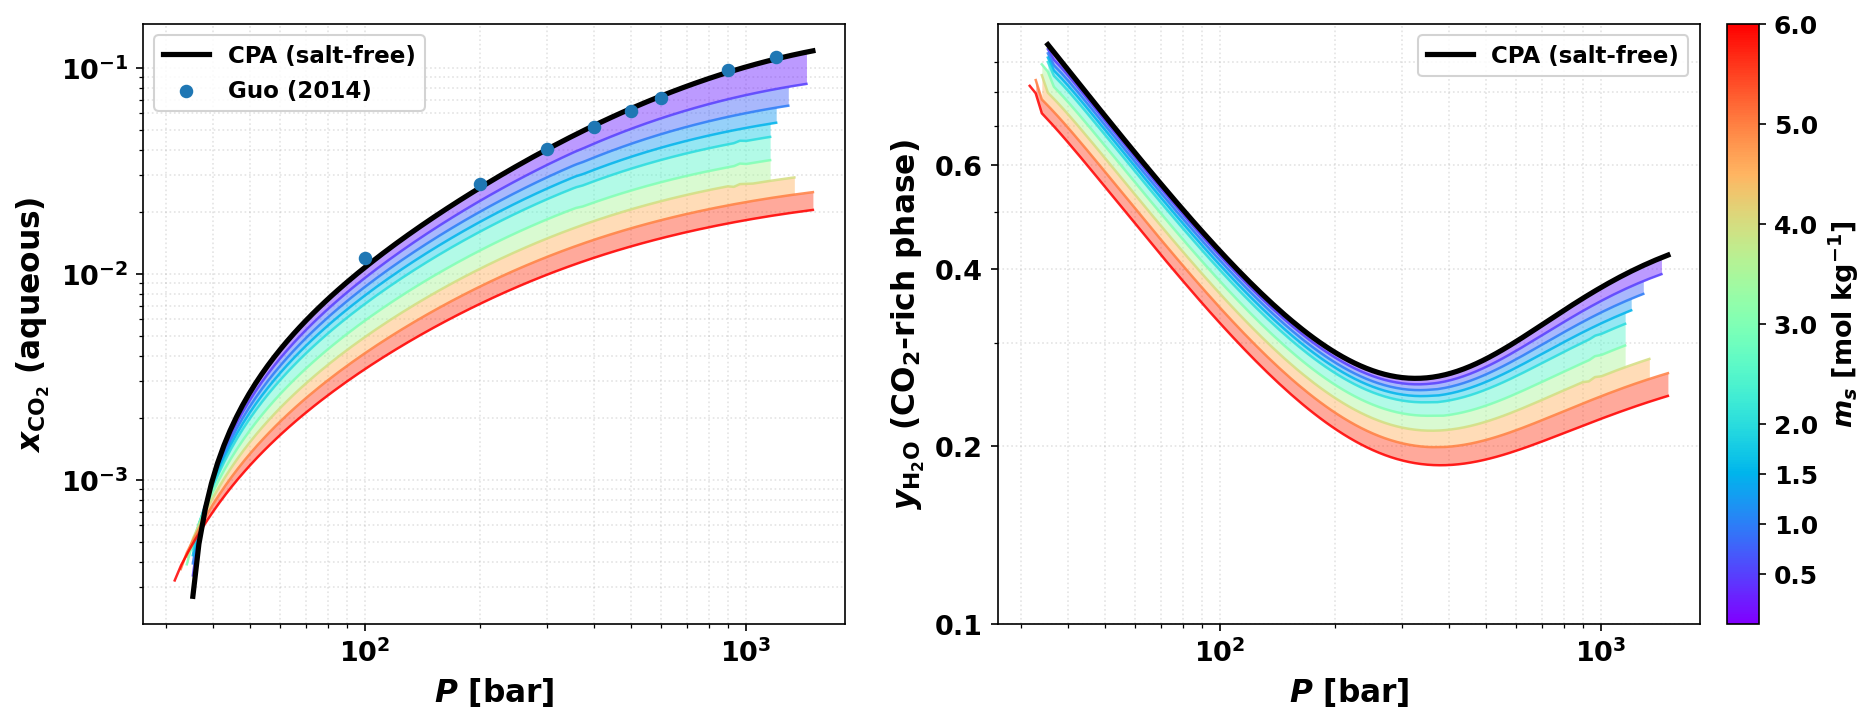
\includegraphics[width=\textwidth]{fig_S1t.png}\caption{$240\,^\circ$C\,(513\,K)}\end{subfigure}\\[6pt]
  \begin{subfigure}[t]{0.8\textwidth}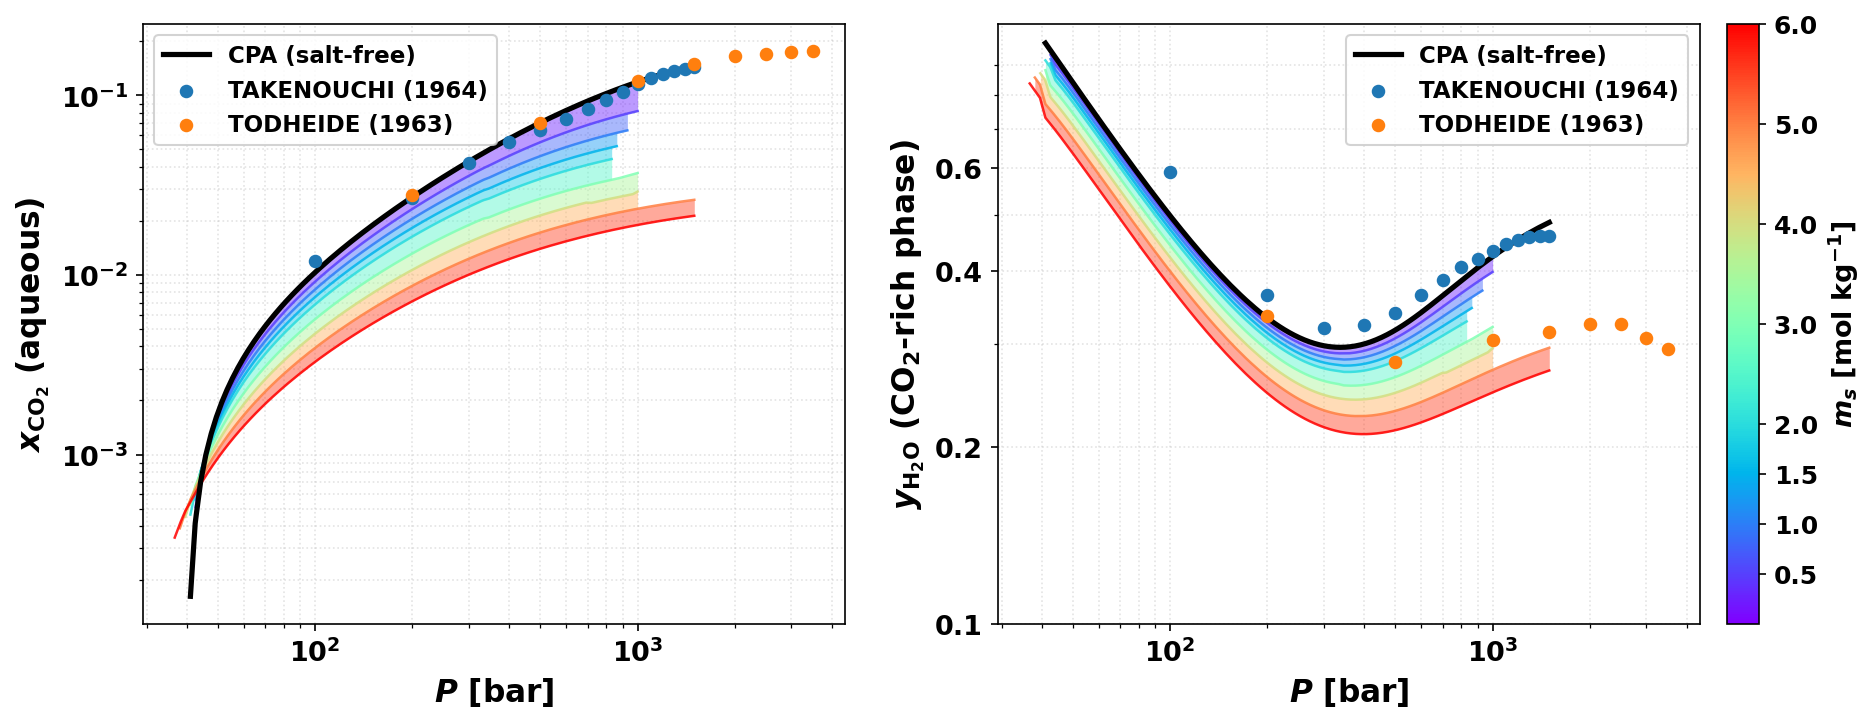
\includegraphics[width=\textwidth]{fig_S1u.png}\caption{$260\,^\circ$C\,(533\,K)}\end{subfigure}
  \caption{(\emph{continued})}
\end{figure}

%% Page 9: 265–275°C
\begin{figure}[H]\ContinuedFloat
  \centering
  \begin{subfigure}[t]{0.8\textwidth}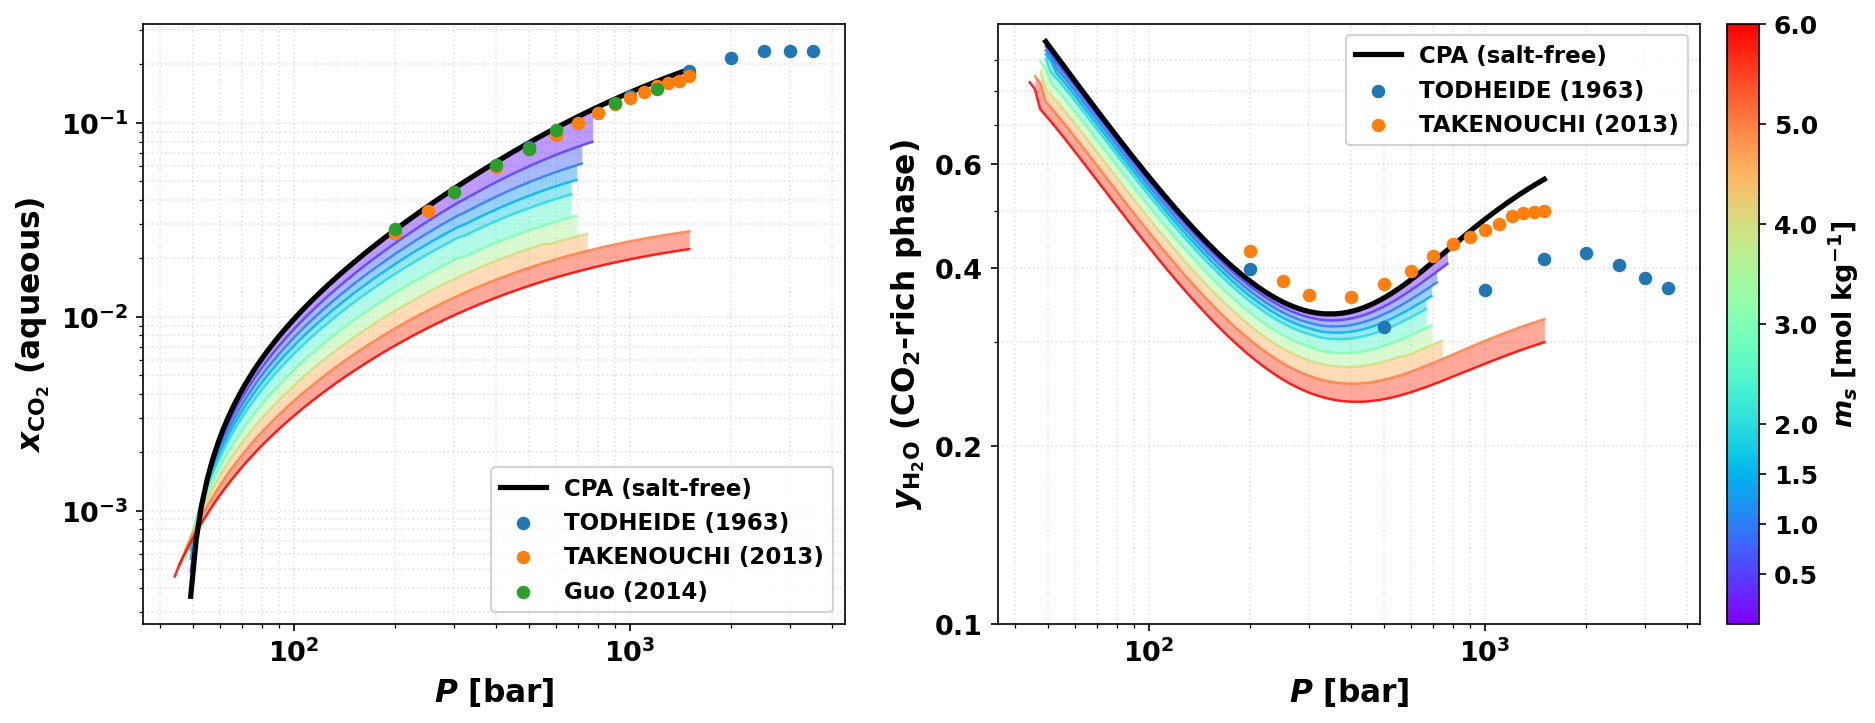
\includegraphics[width=\textwidth]{fig_S1v.png}\caption{$265\,^\circ$C\,(538\,K)}\end{subfigure}\\[6pt]
  \begin{subfigure}[t]{0.8\textwidth}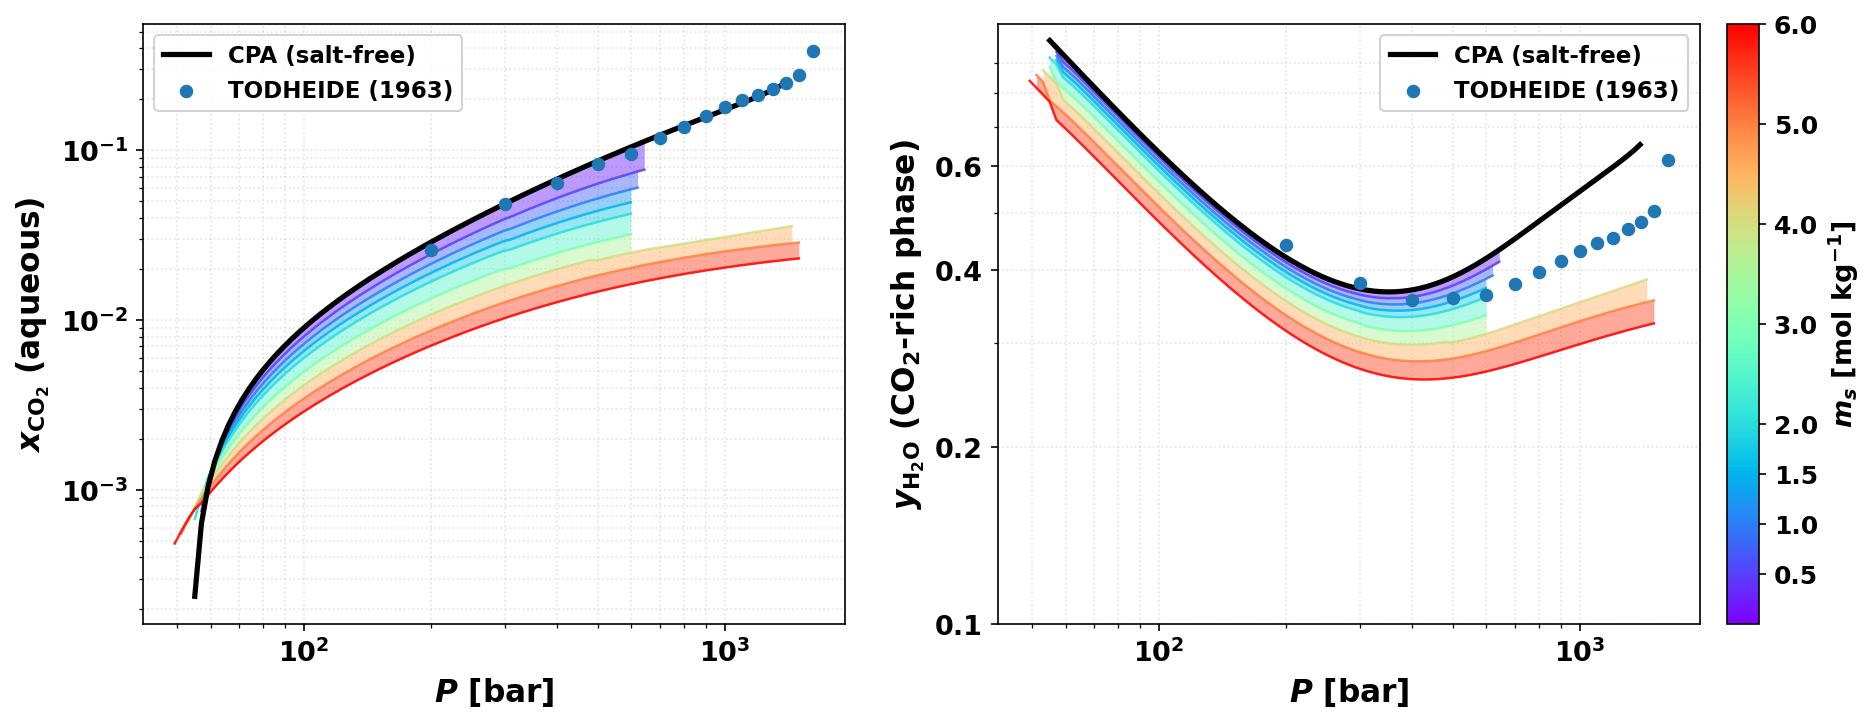
\includegraphics[width=\textwidth]{fig_S1w.png}\caption{$268\,^\circ$C\,(541\,K)}\end{subfigure}\\[6pt]
  \begin{subfigure}[t]{0.8\textwidth}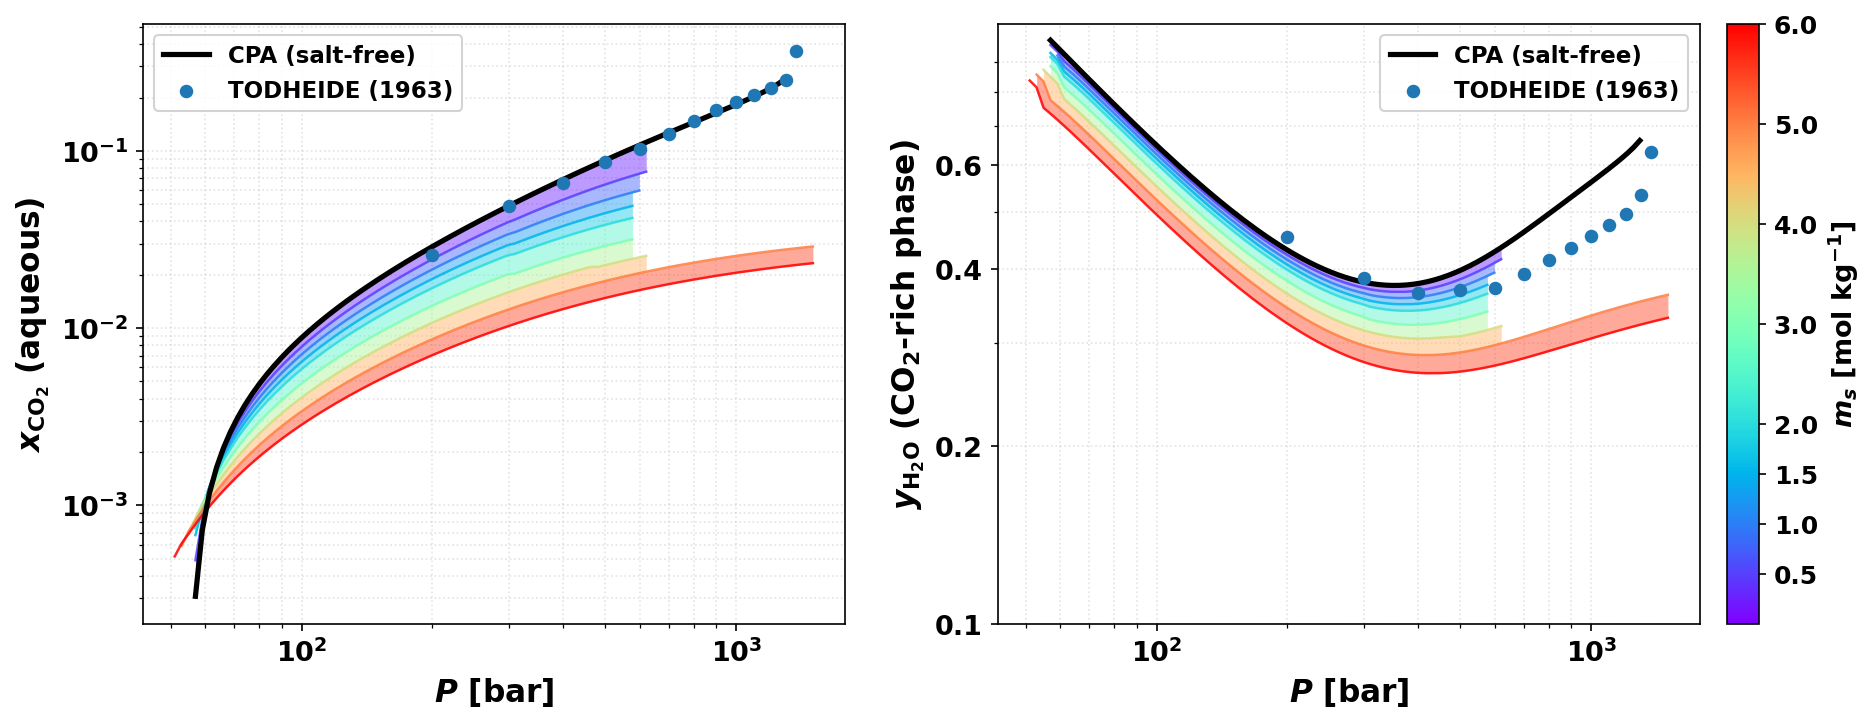
\includegraphics[width=\textwidth]{fig_S1x.png}\caption{$270\,^\circ$C\,(543\,K)}\end{subfigure}
  \caption{(\emph{continued})}
\end{figure}

%% Page 10: 275–300°C
\begin{figure}[H]\ContinuedFloat
  \centering
  \begin{subfigure}[t]{0.8\textwidth}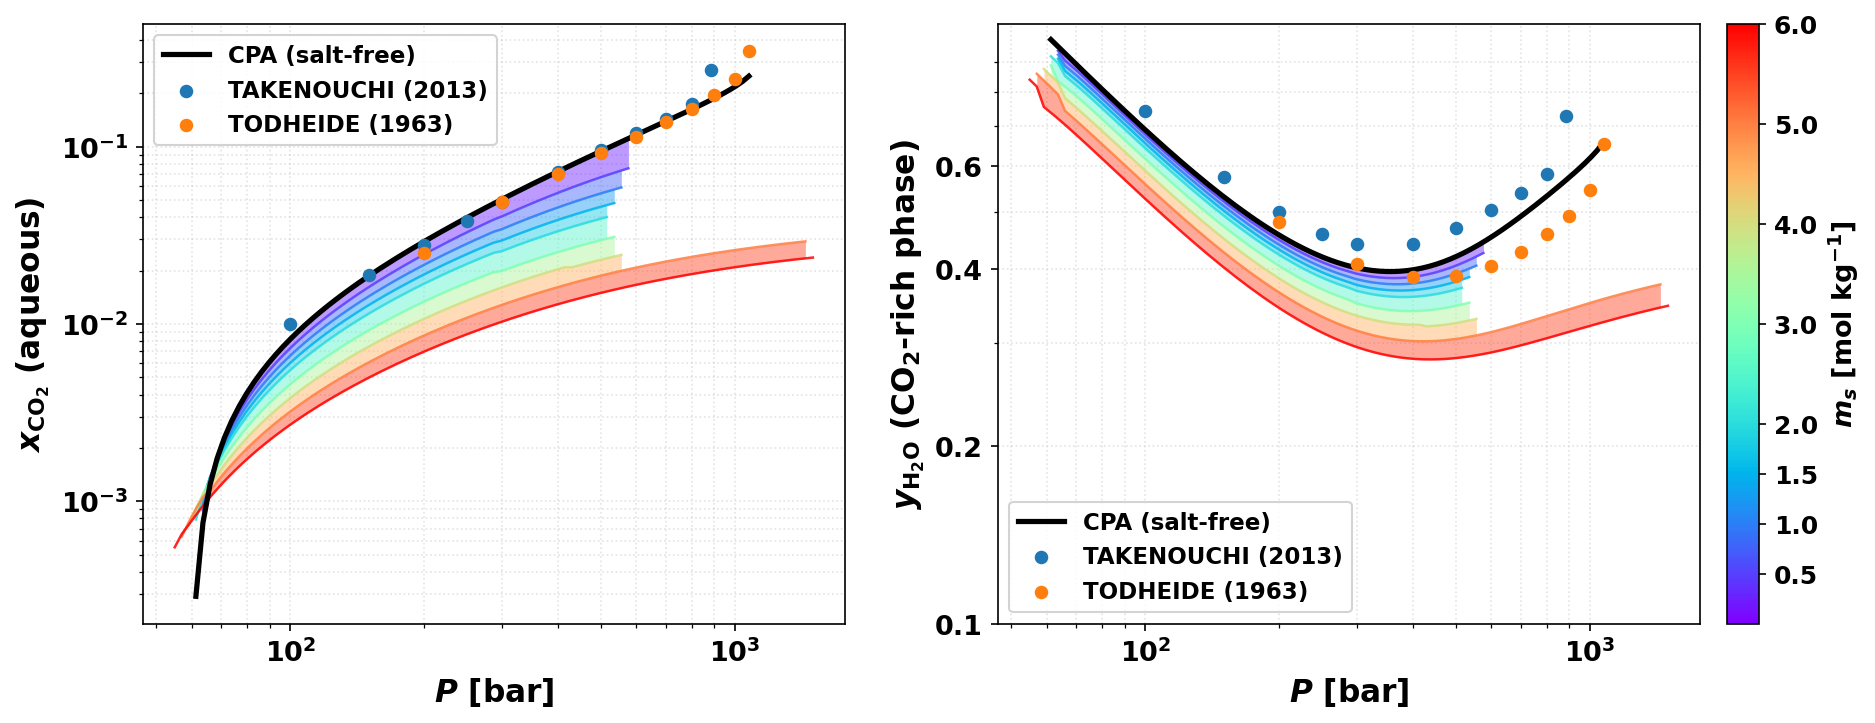
\includegraphics[width=\textwidth]{fig_S1y.png}\caption{$275\,^\circ$C\,(548\,K)}\end{subfigure}\\[6pt]
  \begin{subfigure}[t]{0.8\textwidth}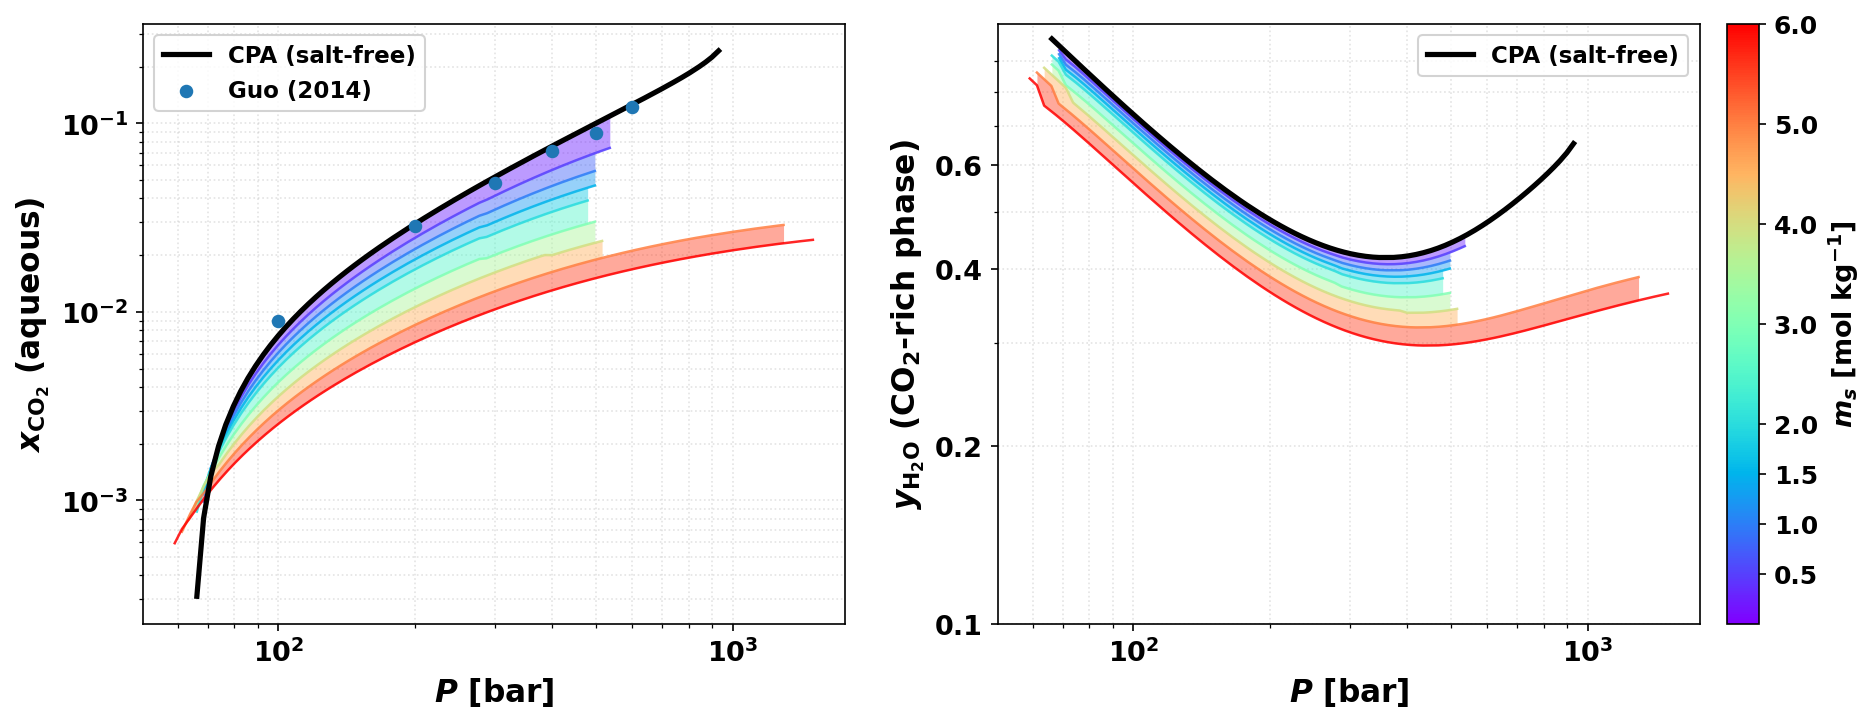
\includegraphics[width=\textwidth]{fig_S1z.png}\caption{$280\,^\circ$C\,(553\,K)}\end{subfigure}\\[6pt]
  \begin{subfigure}[t]{0.8\textwidth}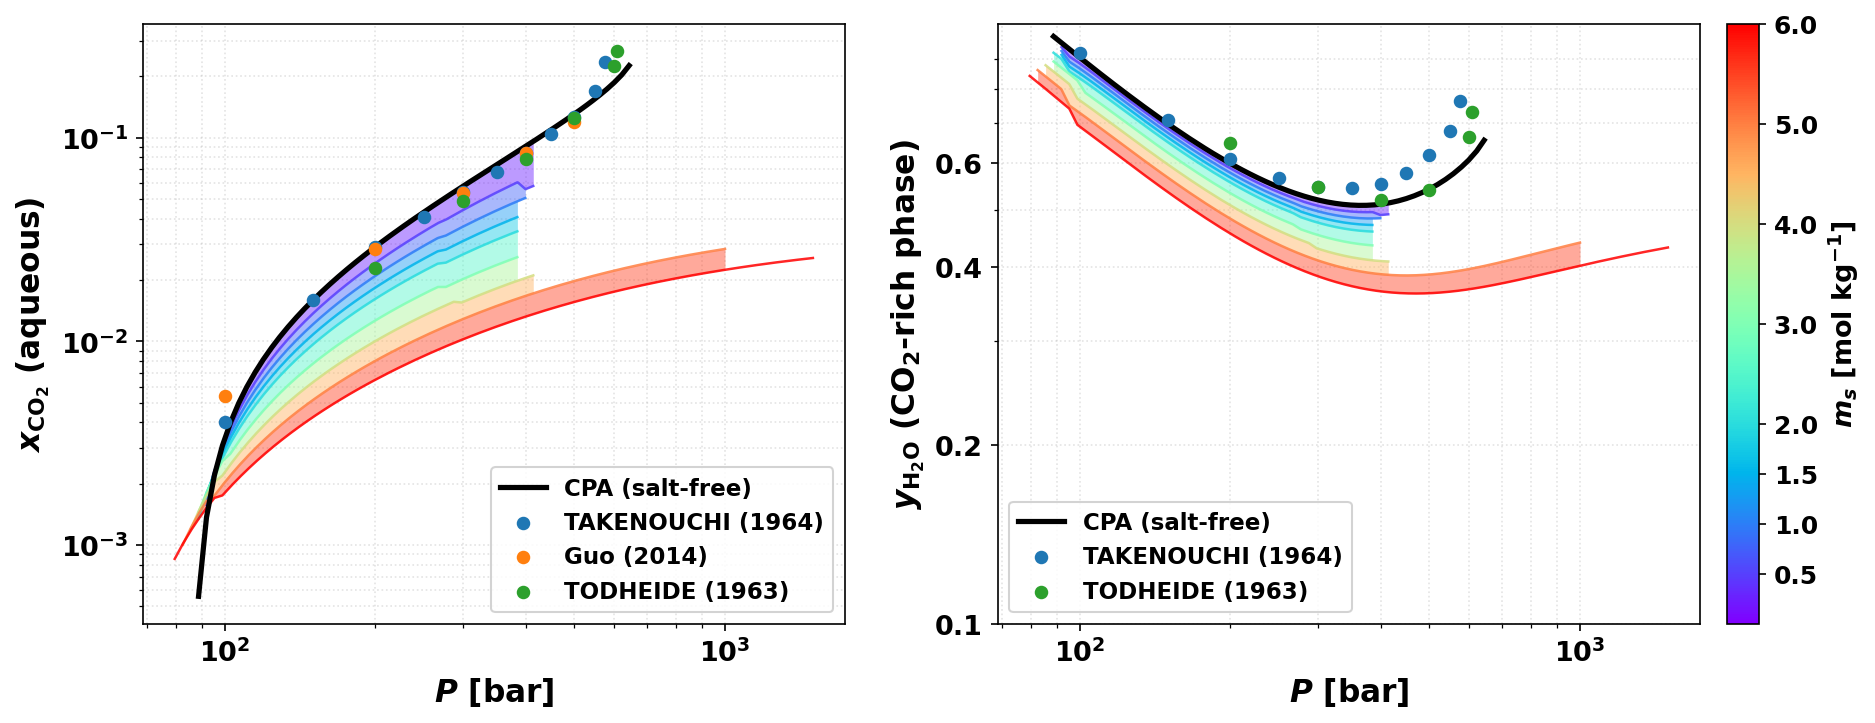
\includegraphics[width=\textwidth]{fig_S1aa.png}\caption{$300\,^\circ$C\,(573\,K)}\end{subfigure}
  \caption{(\emph{continued})}
\end{figure}

%% Page 11: 325–350°C
\begin{figure}[H]\ContinuedFloat
  \centering
  \begin{subfigure}[t]{0.8\textwidth}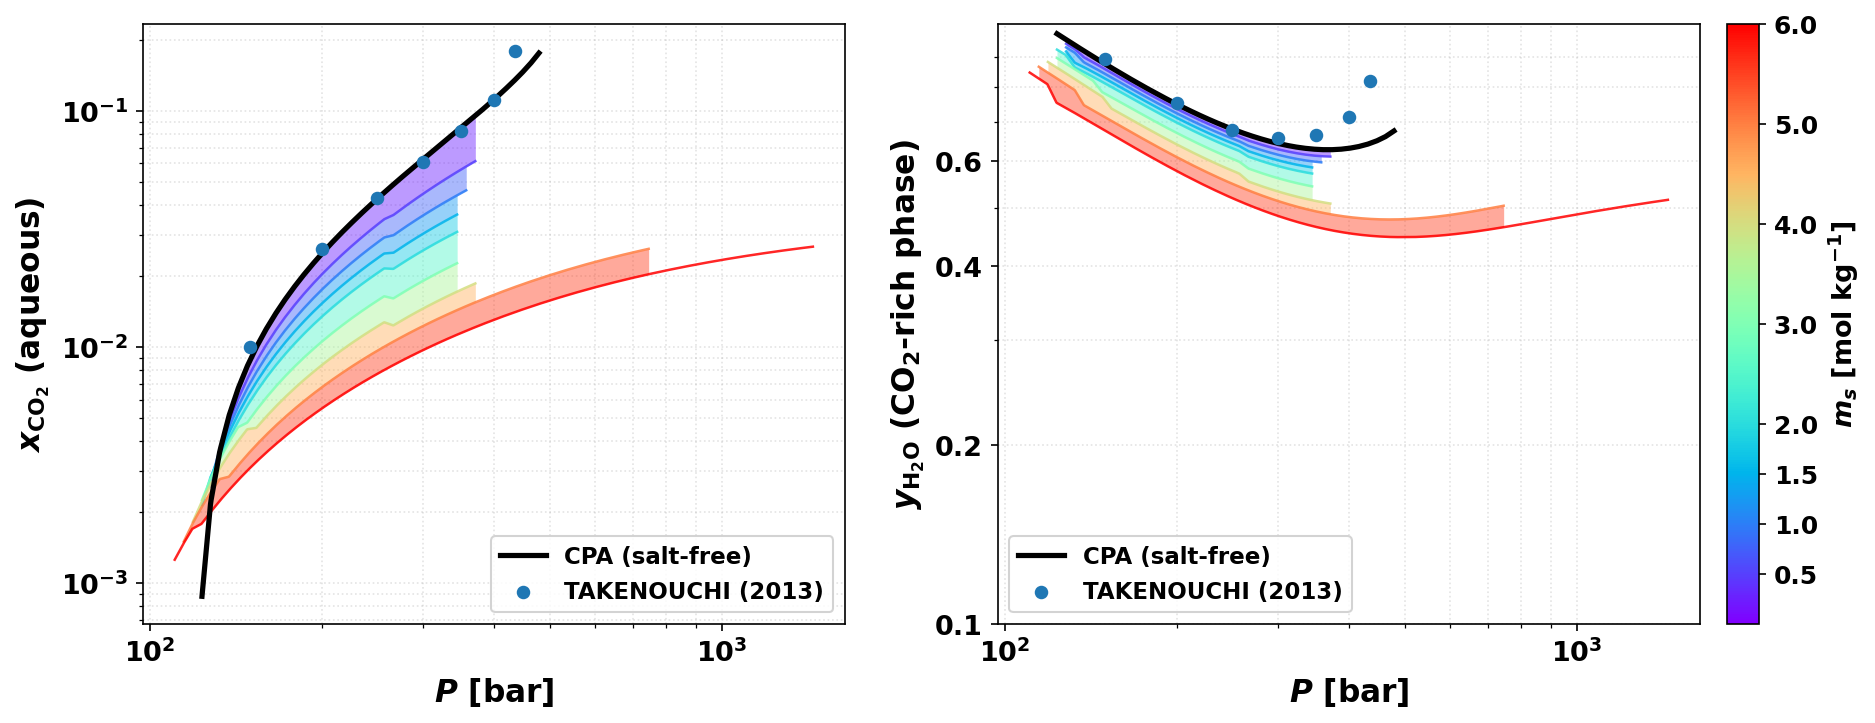
\includegraphics[width=\textwidth]{fig_S1ab.png}\caption{$325\,^\circ$C\,(598\,K)}\end{subfigure}\\[6pt]
  \begin{subfigure}[t]{0.8\textwidth}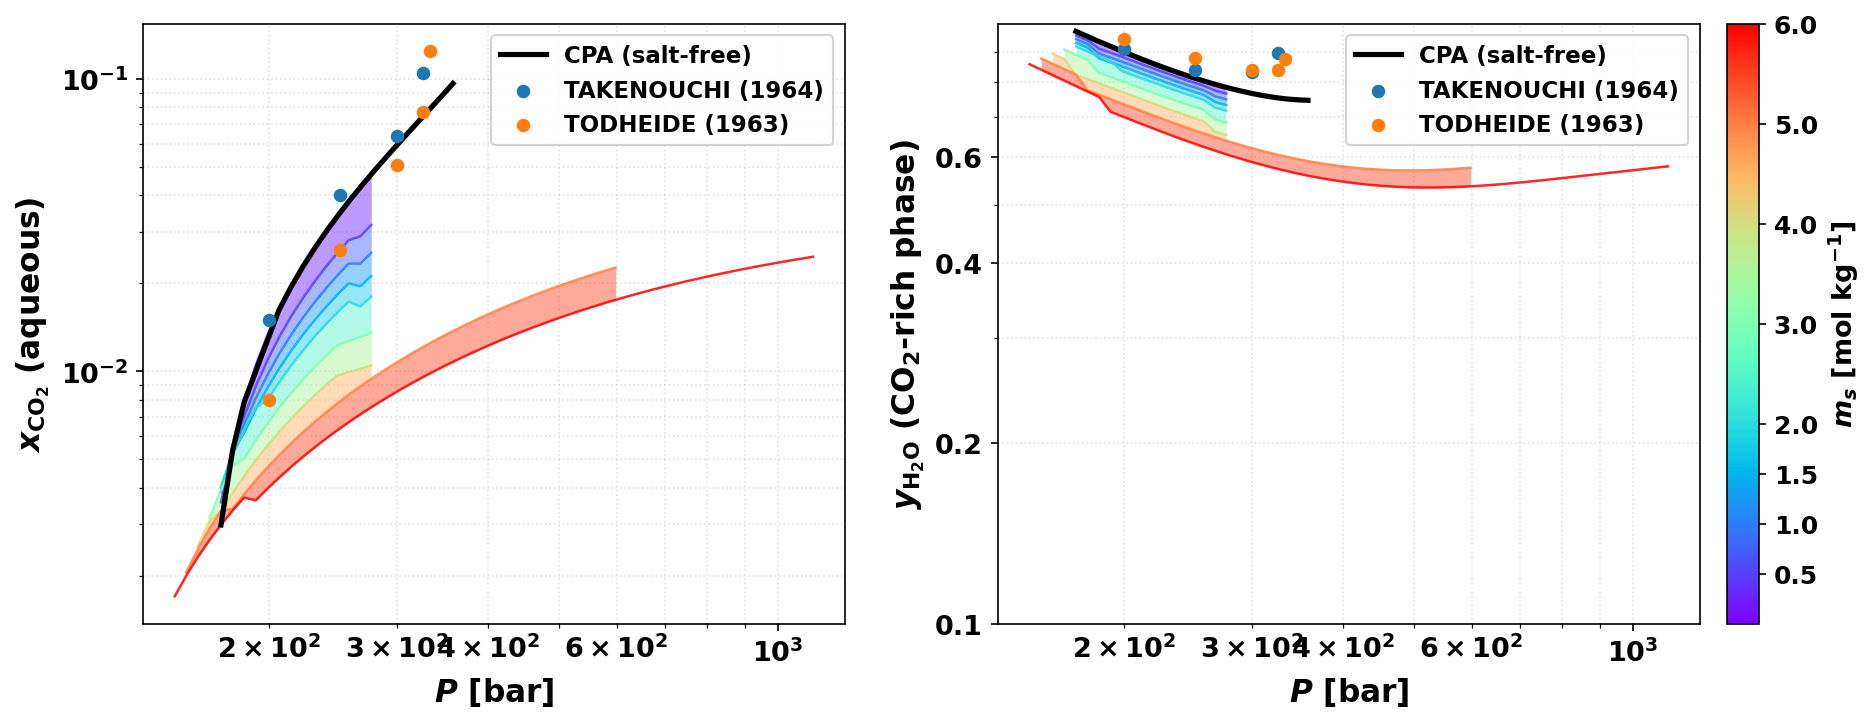
\includegraphics[width=\textwidth]{fig_S1ac.png}\caption{$350\,^\circ$C\,(623\,K)}\end{subfigure}
  \caption{(\emph{continued})}
\end{figure}

%% --- SI Figure S2: remaining single-panel CO2+NaCl panels (2 per row, multi-page) ---
%% Page 1: 5–45°C (3 rows)
\begin{figure}[H]
  \centering
  \newcommand{\snwsi}{0.47\textwidth}%
  \begin{subfigure}[t]{\snwsi}\centering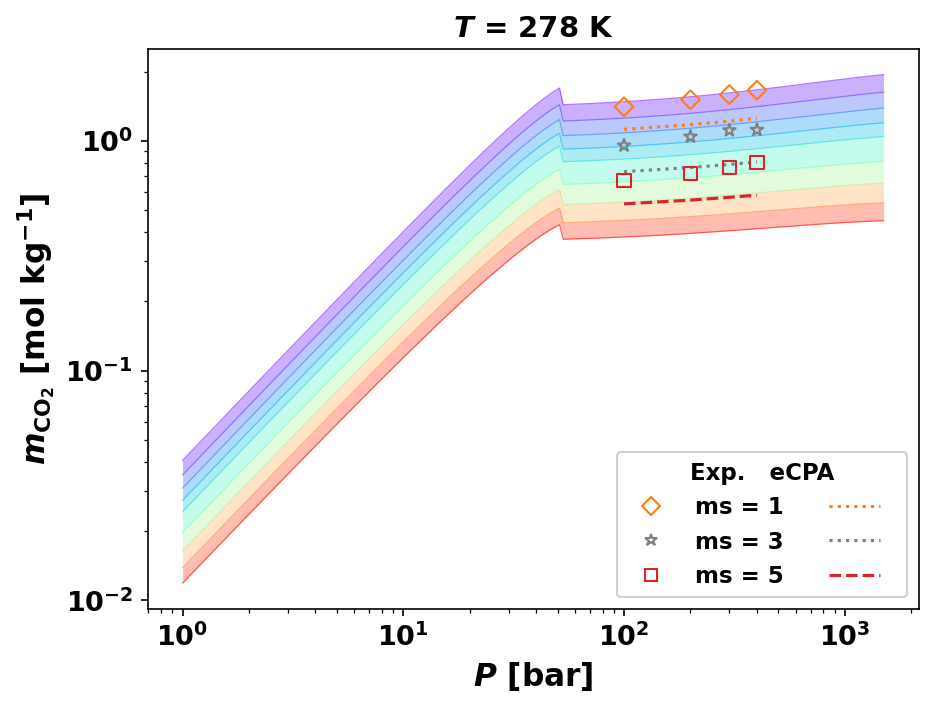
\includegraphics[width=.9\textwidth]{fig_S2a.png}\caption{$5\,^\circ$C}\end{subfigure}\hfill
  \begin{subfigure}[t]{\snwsi}\centering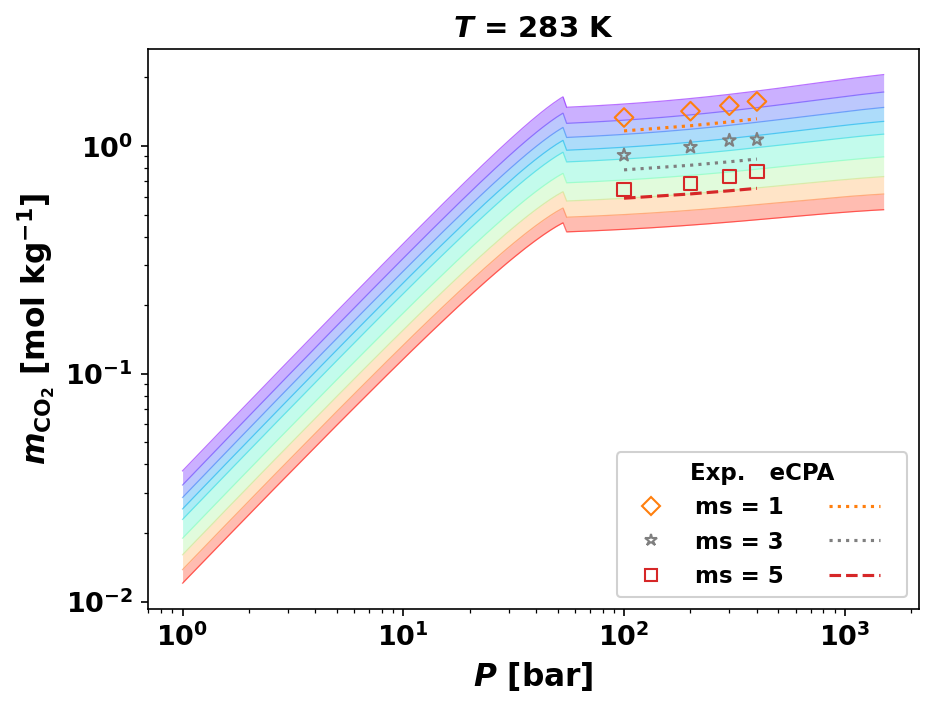
\includegraphics[width=.9\textwidth]{fig_S2b.png}\caption{$10\,^\circ$C}\end{subfigure}\\[6pt]
  \begin{subfigure}[t]{\snwsi}\centering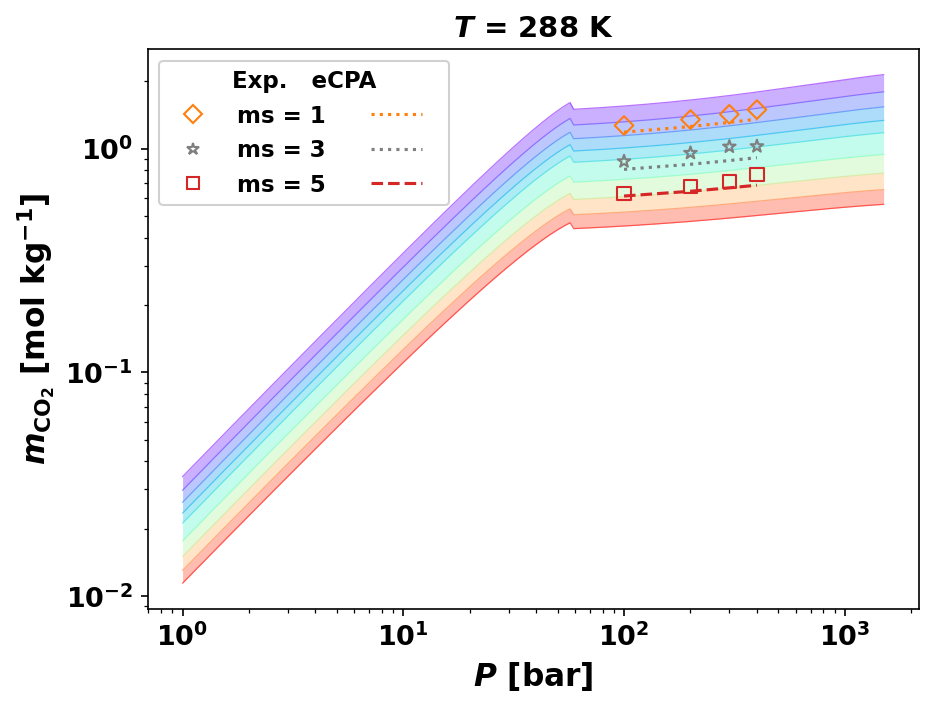
\includegraphics[width=.9\textwidth]{fig_S2c.png}\caption{$15\,^\circ$C}\end{subfigure}\hfill
  \begin{subfigure}[t]{\snwsi}\centering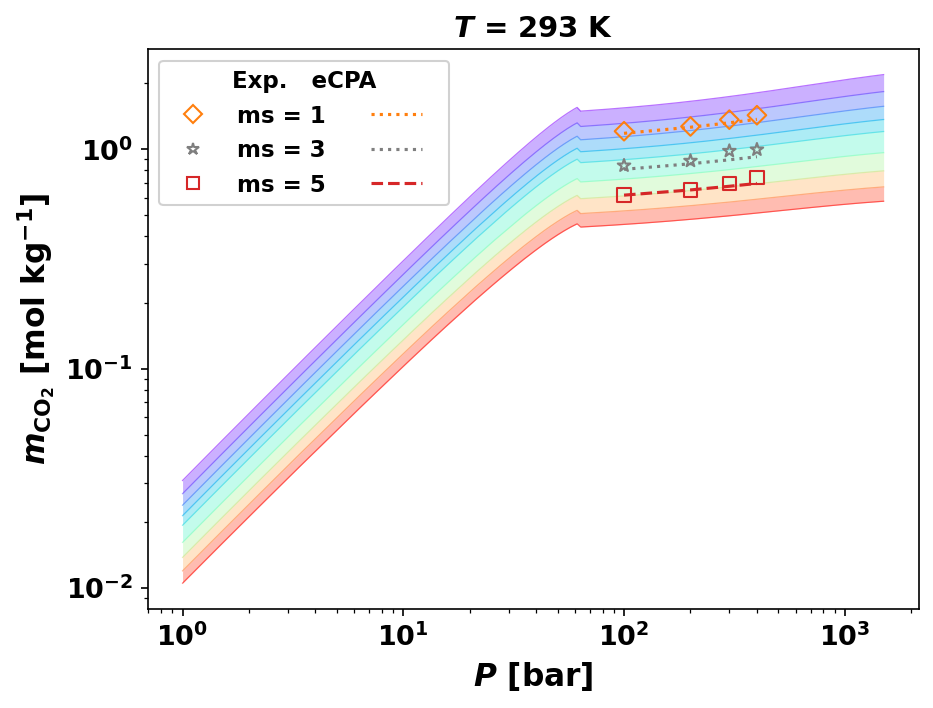
\includegraphics[width=.9\textwidth]{fig_S2d.png}\caption{$20\,^\circ$C}\end{subfigure}\\[6pt]
  \begin{subfigure}[t]{\snwsi}\centering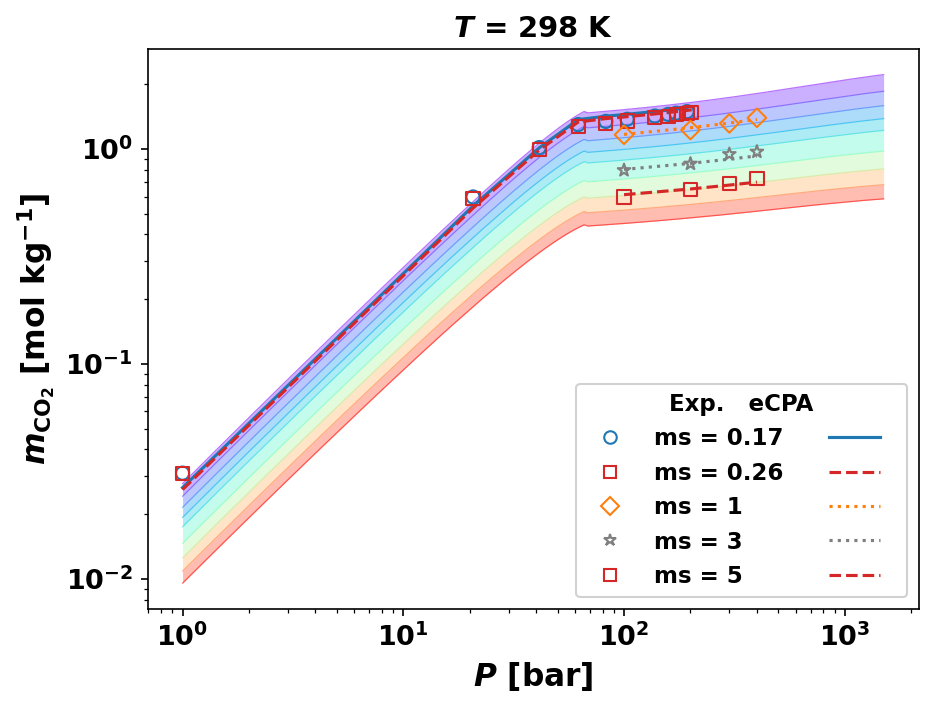
\includegraphics[width=.9\textwidth]{fig_2a.png}\caption{$25\,^\circ$C}\end{subfigure}\hfill
  \begin{subfigure}[t]{\snwsi}\centering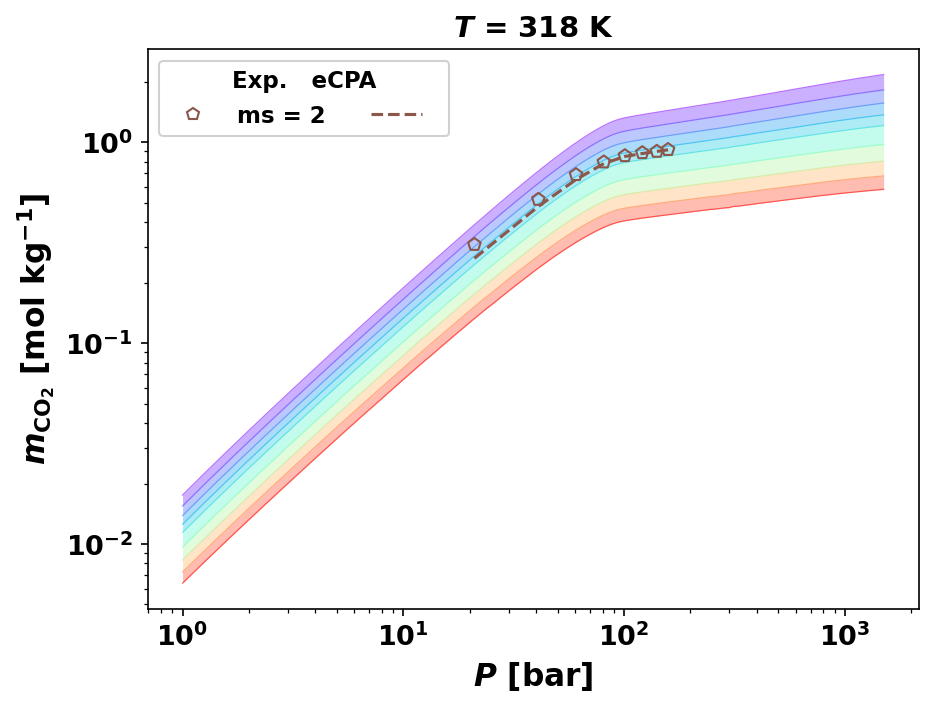
\includegraphics[width=.9\textwidth]{fig_S2e.png}\caption{$45\,^\circ$C}\end{subfigure}
  \caption{CO$_2$ solubility in NaCl brine at thirteen temperatures not shown in
           Fig.~2 of the main text ($5$--$350\,^\circ$C), including data at high NaCl molalities
           up to $m_s = 6$\,mol\,kg$^{-1}$ from multiple sources.
           Each panel shows CO$_2$ molality $m_{\text{CO}_2}$ [mol\,kg$^{-1}$] vs.\ pressure (log--log).
           Open symbols: experimental data \citep{Guo2015, Rumpf1994, Bando2003,
           Chabab2020, Liu2021, Liu2011b, Nighswander1989, Takenouchi1965, Yan2011};
           discrete lines with markers: eCPA at the experimental NaCl molalities.
           Rainbow-colored background bands: continuous eCPA predictions across
           $m_s = 0$--$6$\,mol\,kg$^{-1}$ (color scale as in Fig.~1 of the main text).
           At $T \geq 400\,^\circ$C, eCPA predicts single-phase (fully miscible) behavior
           for all available experimental pressures.}
  \label{fig:co2nacl_Tpanel_SI}
\end{figure}

%% Page 2: 60–200°C
\begin{figure}[H]\ContinuedFloat
  \centering
  \newcommand{\snwsib}{0.47\textwidth}%
  \begin{subfigure}[t]{\snwsib}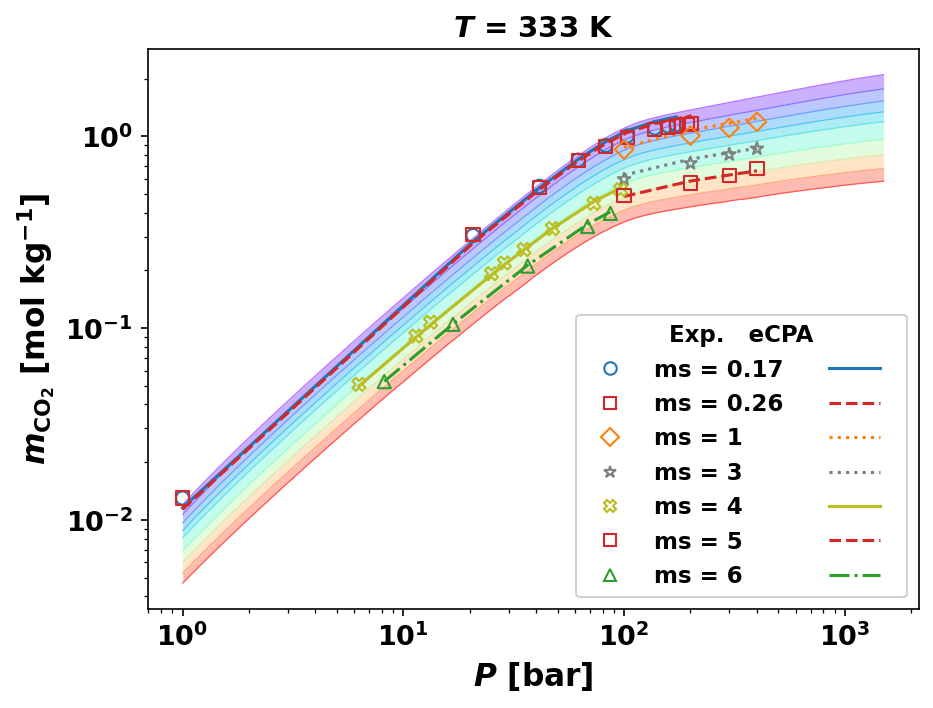
\includegraphics[width=\textwidth]{fig_S2f.png}\caption{$60\,^\circ$C}\end{subfigure}\hfill
  \begin{subfigure}[t]{\snwsib}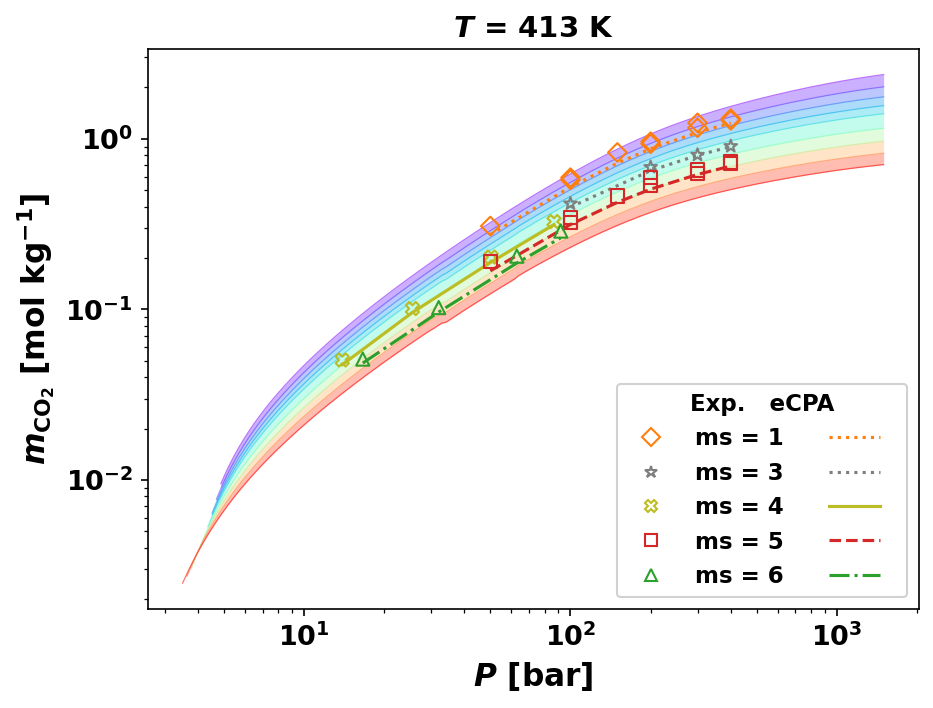
\includegraphics[width=\textwidth]{fig_S2g.png}\caption{$140\,^\circ$C}\end{subfigure}\\[6pt]
  \begin{subfigure}[t]{\snwsib}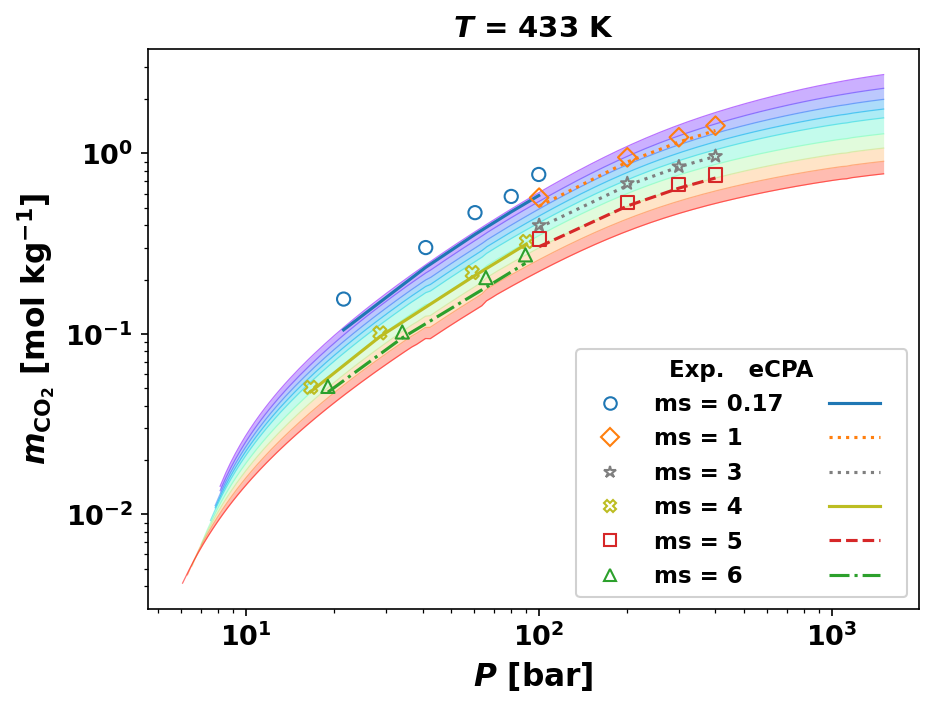
\includegraphics[width=\textwidth]{fig_S2h.png}\caption{$160\,^\circ$C}\end{subfigure}\hfill
  \begin{subfigure}[t]{\snwsib}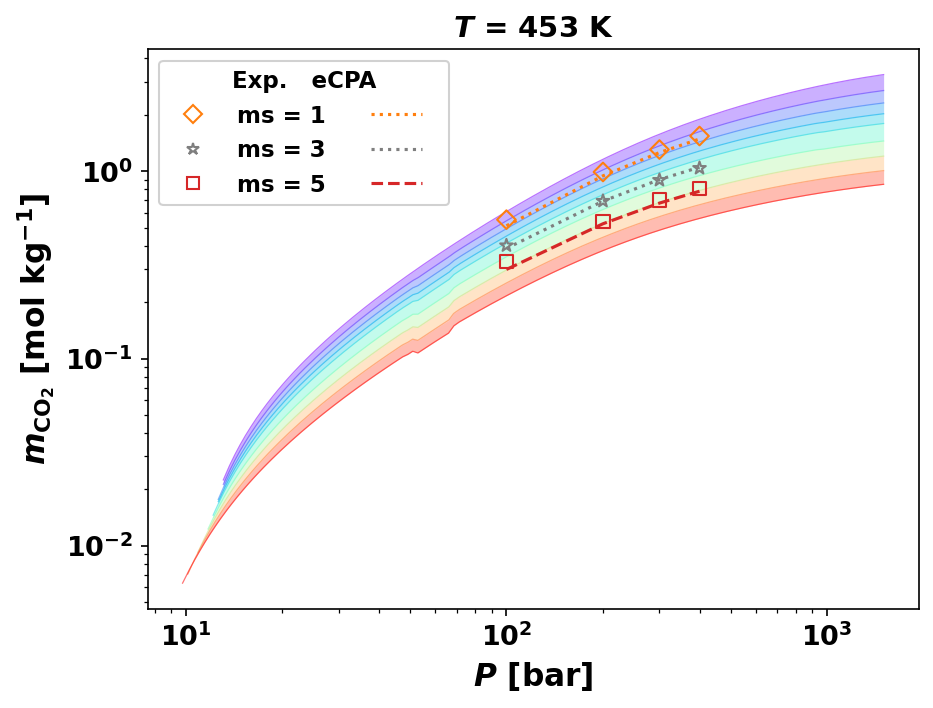
\includegraphics[width=\textwidth]{fig_2e.png}\caption{$180\,^\circ$C}\end{subfigure}\\[6pt]
  \begin{subfigure}[t]{\snwsib}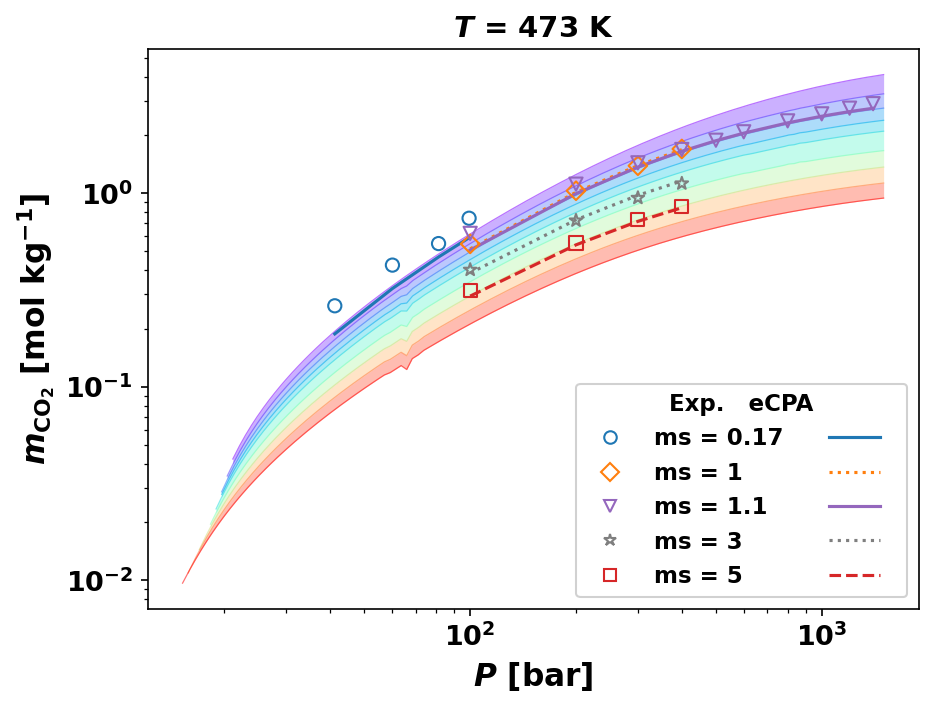
\includegraphics[width=\textwidth]{fig_S2i.png}\caption{$200\,^\circ$C}\end{subfigure}
  \caption{(\emph{continued})}
\end{figure}

%% Page 3: 300–350°C (hydrothermal)
\begin{figure}[H]\ContinuedFloat
  \centering
  \newcommand{\snwsic}{0.47\textwidth}%
  \begin{subfigure}[t]{\snwsic}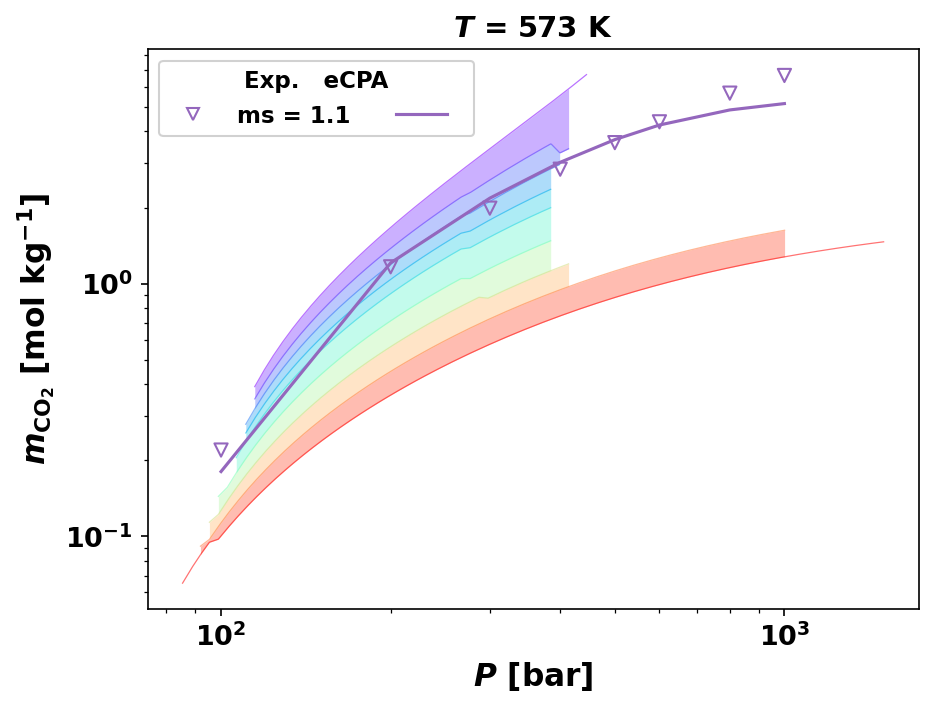
\includegraphics[width=\textwidth]{fig_S3a.png}\caption{$300\,^\circ$C}\end{subfigure}\hfill
  \begin{subfigure}[t]{\snwsic}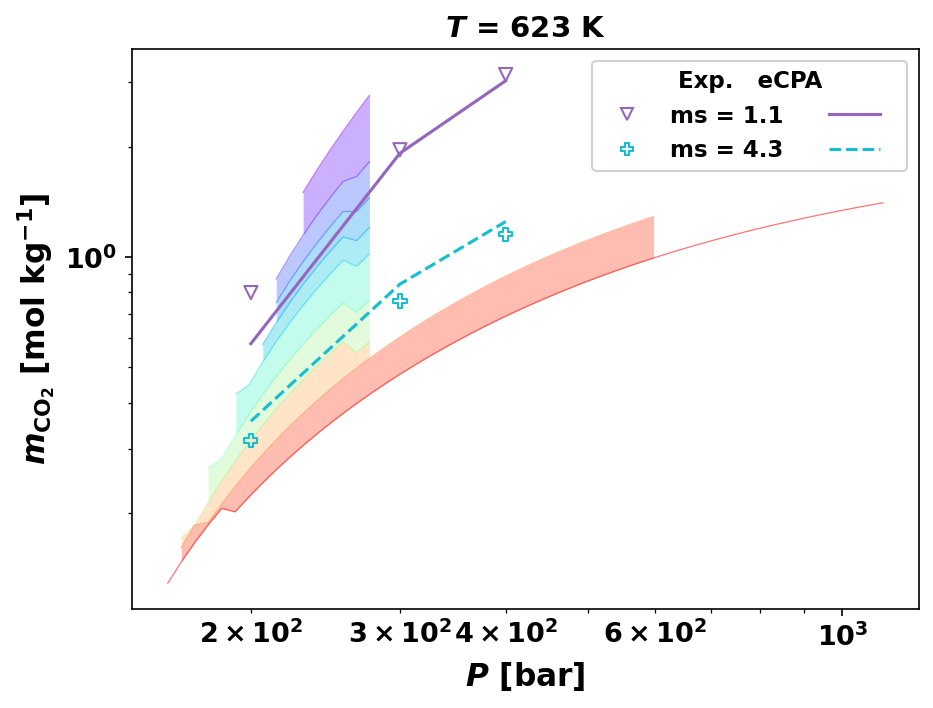
\includegraphics[width=\textwidth]{fig_S3b.png}\caption{$350\,^\circ$C}\end{subfigure}
  \caption{(\emph{continued})}
\end{figure}

%% --- SI Figure S3: two-panel CO2+NaCl at 100°C (molality + CO2-rich phase) ---
\begin{figure}[H]
  \centering
  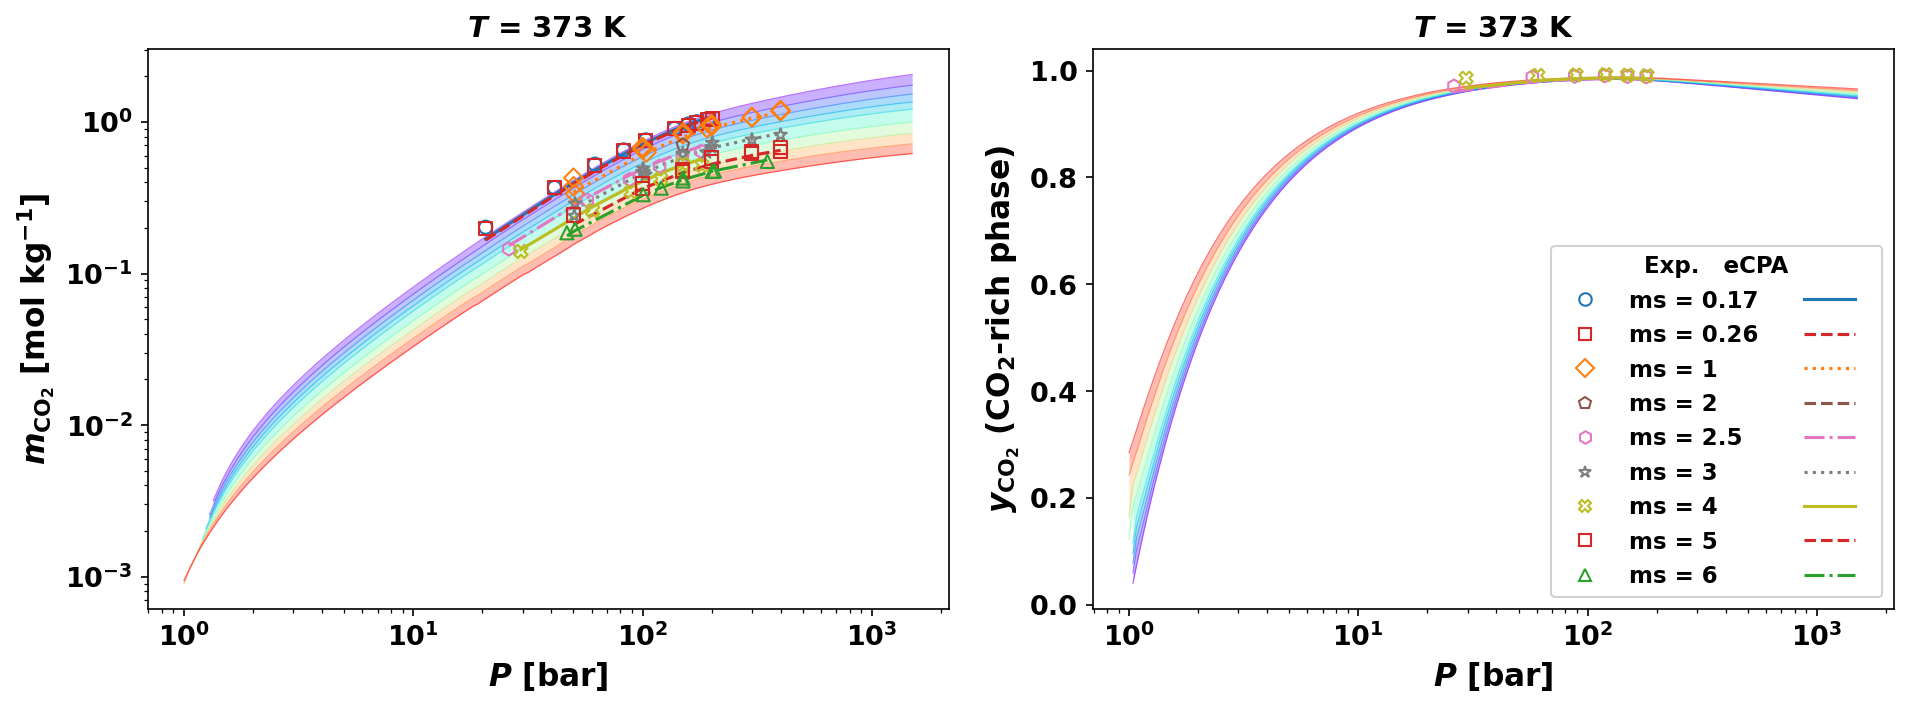
\includegraphics[width=0.9\textwidth]{fig_3b.png}
  \caption{CO$_2$ + NaCl brine phase equilibria at $T = 100\,^\circ$C for which both
           CO$_2$ molality $m_{\text{CO}_2}$ (left panel) and CO$_2$ mole fraction in the
           CO$_2$-rich phase $y_{\text{CO}_2}$ (right panel) data are available.
           Open symbols: experimental data \citep{Bando2003, Chabab2020, Guo2015,
           Hou2013, Koschel2006, Liu2021, Messabeb2016, Savary2012, Takenouchi1965,
           Yan2011, Zhao2015}; discrete lines with markers: eCPA at the experimental
           NaCl molalities.
           Rainbow-colored background bands: continuous eCPA predictions across
           $m_s = 0$--$6$\,mol\,kg$^{-1}$ (color scale as in Fig.~1 of the main text).}
  \label{fig:co2nacl_2panel_SI}
\end{figure}

\begin{figure}[H]
  \centering
  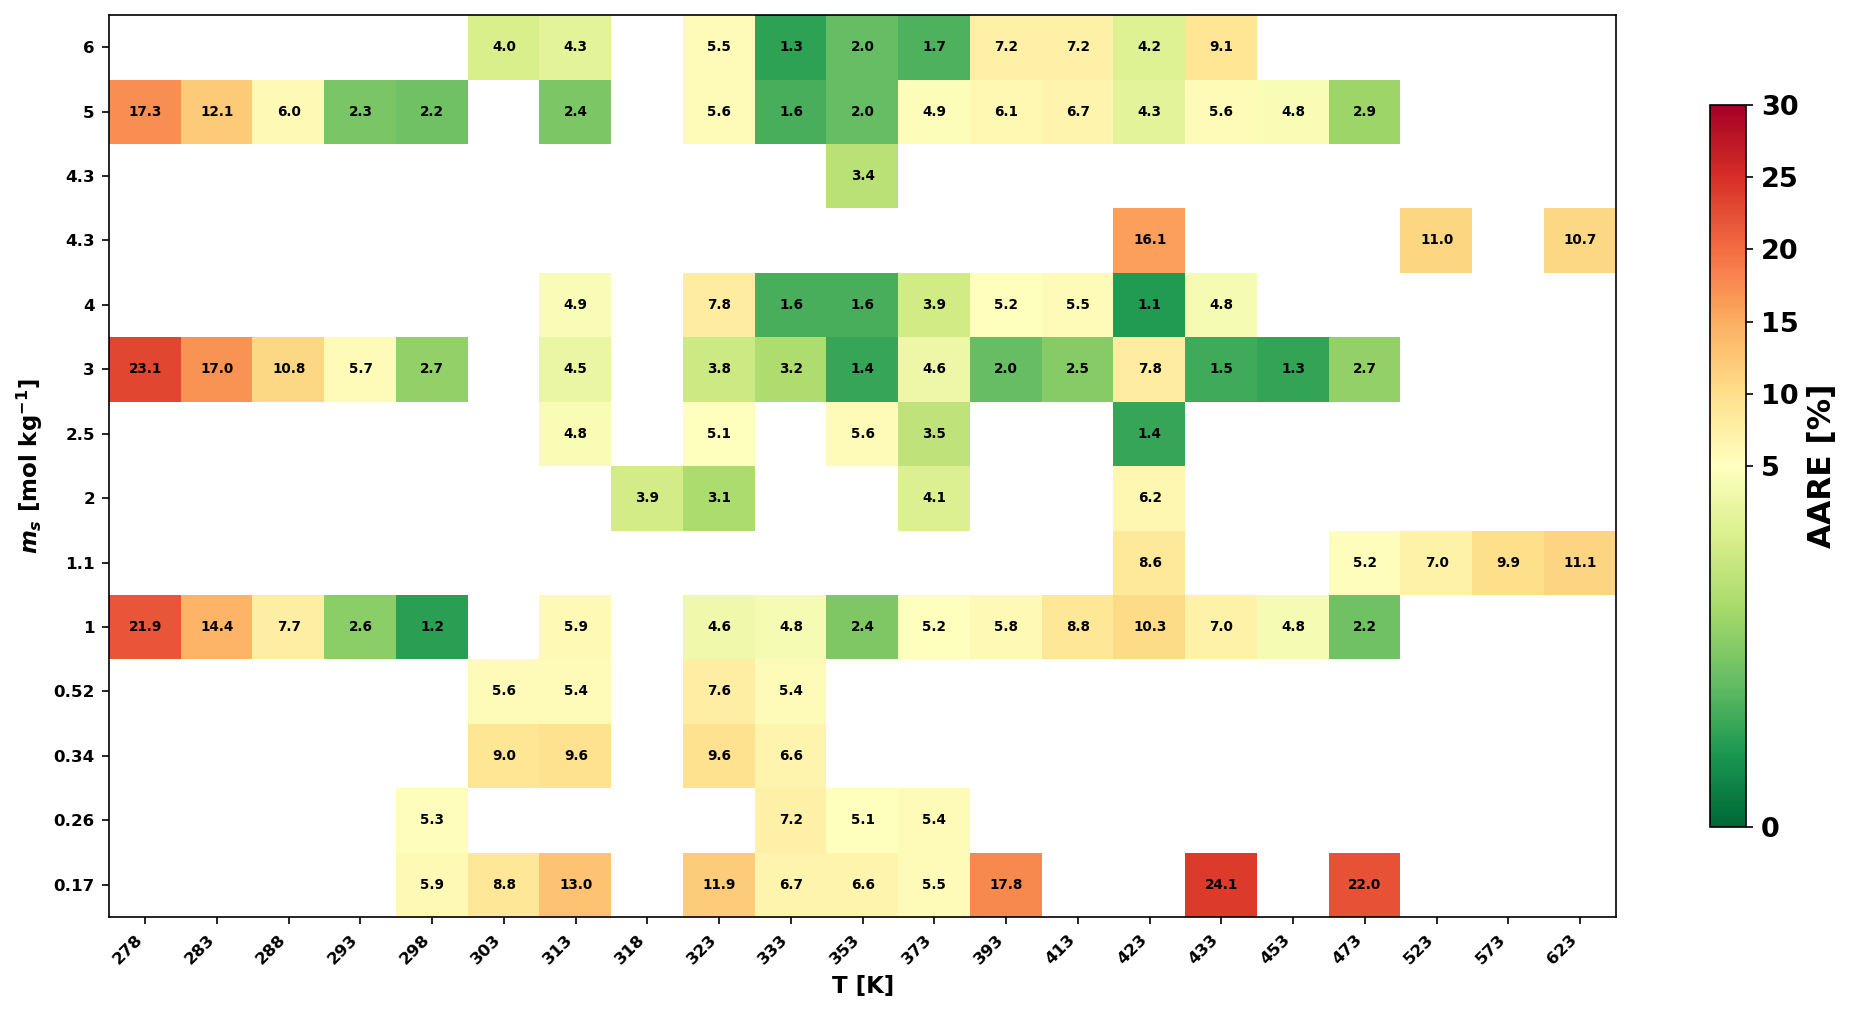
\includegraphics[width=0.95\textwidth]{fig_S4.png}
  \caption{Heatmap of absolute relative error (AARE, \%) for the CO$_2$ + NaCl
           validation dataset ($T = 5$--$350\,^\circ$C), showing all individual NaCl
           molalities present in the experimental data.
           Color scale is diverging at 5\%: green $\leq 5\%$, red $\geq 10\%$.
           Empty cells indicate no experimental data at that $(T, m_s)$ combination.}
  \label{fig:co2nacl_heatmap}
\end{figure}

\subsection{Aqueous-phase density: extended validation}
\label{sec:density_si}

We validate pure-water CPA/eCPA density (with the temperature-dependent Péneloux shift,
Section~\ref{sec:params}) against the IAPWS-95 international standard \citep{IAPWS2016},
whose documented uncertainty in liquid-water density is $\pm0.001$--$0.02\%$
\citep{IAPWS2016} — well below the eCPA model error — over a systematic grid of 26 temperatures ($T = 0$--$350\,^\circ$C) and 20 pressures
($P = 1$--$2\,000$\,bar), restricted to liquid/compressed-water conditions (475 points;
vapour excluded).
The eCPA density is $\rho = M_{\text{H}_2\text{O}}\,/\,(Z^{\rm aq} RT/P + c_{\text{H}_2\text{O}}(T))$,
where $c_{\text{H}_2\text{O}}(T)$ is the polynomial from Section~\ref{sec:params}.

The parity plot (Fig.~\ref{fig:density}) shows tight agreement across the full range.
The signed error map (Fig.~\ref{fig:density_surface}) is nearly flat, with residual
errors $< 0.7\%$ at most conditions; the largest deviations ($\approx 3\%$) occur near
$350\,^\circ$C, close to the critical point of water, where cubic-EoS predictions are
least accurate.
Overall: AARE = 0.30\%, bias = $-$0.20\%, maximum ARE = 3.0\% (475 liquid conditions).
For subsurface CO$_2$ storage conditions ($T \leq 120\,^\circ$C,
$P = 75$--$600$\,bar, $N = 136$), the AARE is 0.12\%.

\begin{figure}[H]
  \centering
  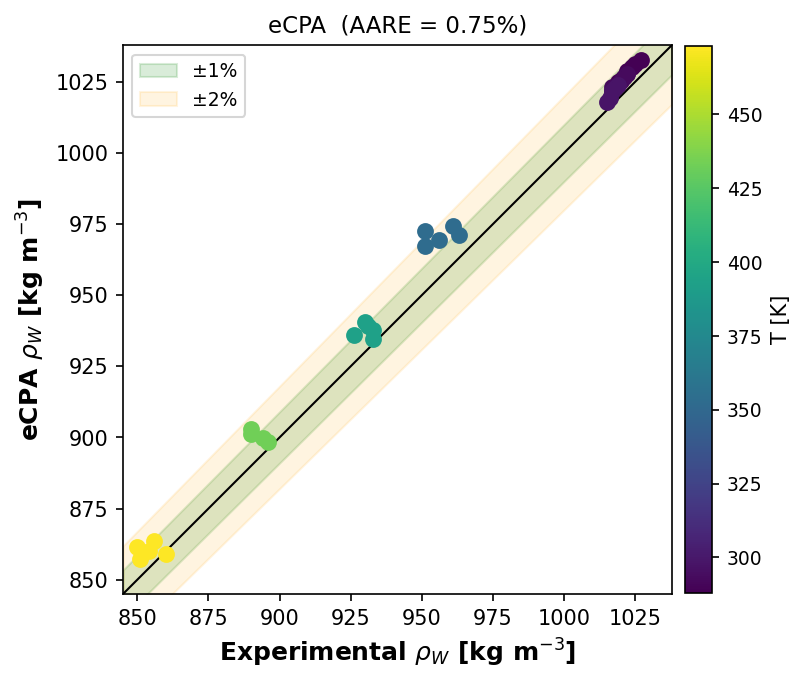
\includegraphics[width=\textwidth]{fig_S5.png}
  \caption{Parity plot: eCPA pure-water density versus IAPWS-95 \citep{IAPWS2016}
           (475 liquid/compressed-water conditions, $T = 0$--$350\,^\circ$C,
           $P = 1$--$2\,000$\,bar).
           Left panel: $P \leq 300$\,bar; right panel: all conditions up to 2\,000\,bar.
           Points are colored by temperature; shaded bands indicate $\pm$1\% and $\pm$2\%
           deviations. The temperature-dependent Péneloux shift (Section~\ref{sec:params})
           is applied.}
  \label{fig:density}
\end{figure}

\begin{figure}[H]
  \centering
  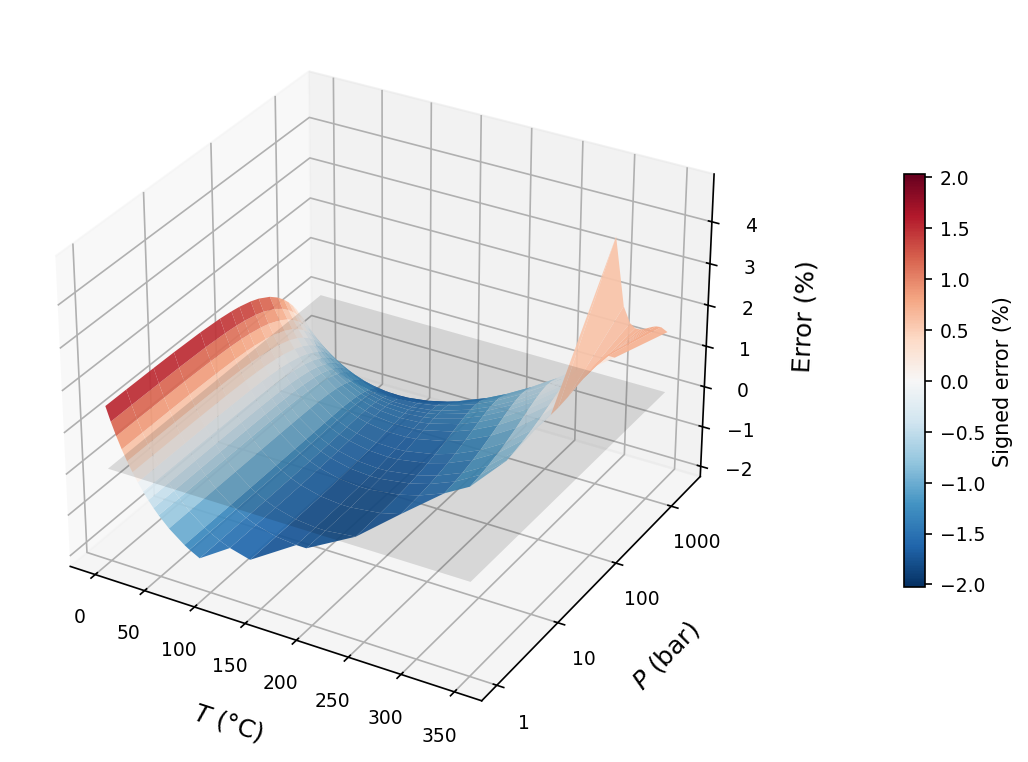
\includegraphics[width=0.90\textwidth]{fig_S5b.png}
  \caption{Signed relative error (eCPA $-$ IAPWS-95) / IAPWS-95 (\%) of pure-water
           density predictions over $T = 0$--$350\,^\circ$C and $P = 1$--$2\,000$\,bar
           (475 liquid/compressed-water conditions; vapour excluded; $P$-axis logarithmic).
           The temperature-dependent Péneloux shift (Section~\ref{sec:params}) is applied.
           The error field is nearly flat ($< 0.7\%$ over most of the domain);
           the largest deviations ($\approx 3\%$) occur near $350\,^\circ$C
           at moderate pressures, close to the critical point of water.}
  \label{fig:density_surface}
\end{figure}

\begin{figure}[H]
  \centering
  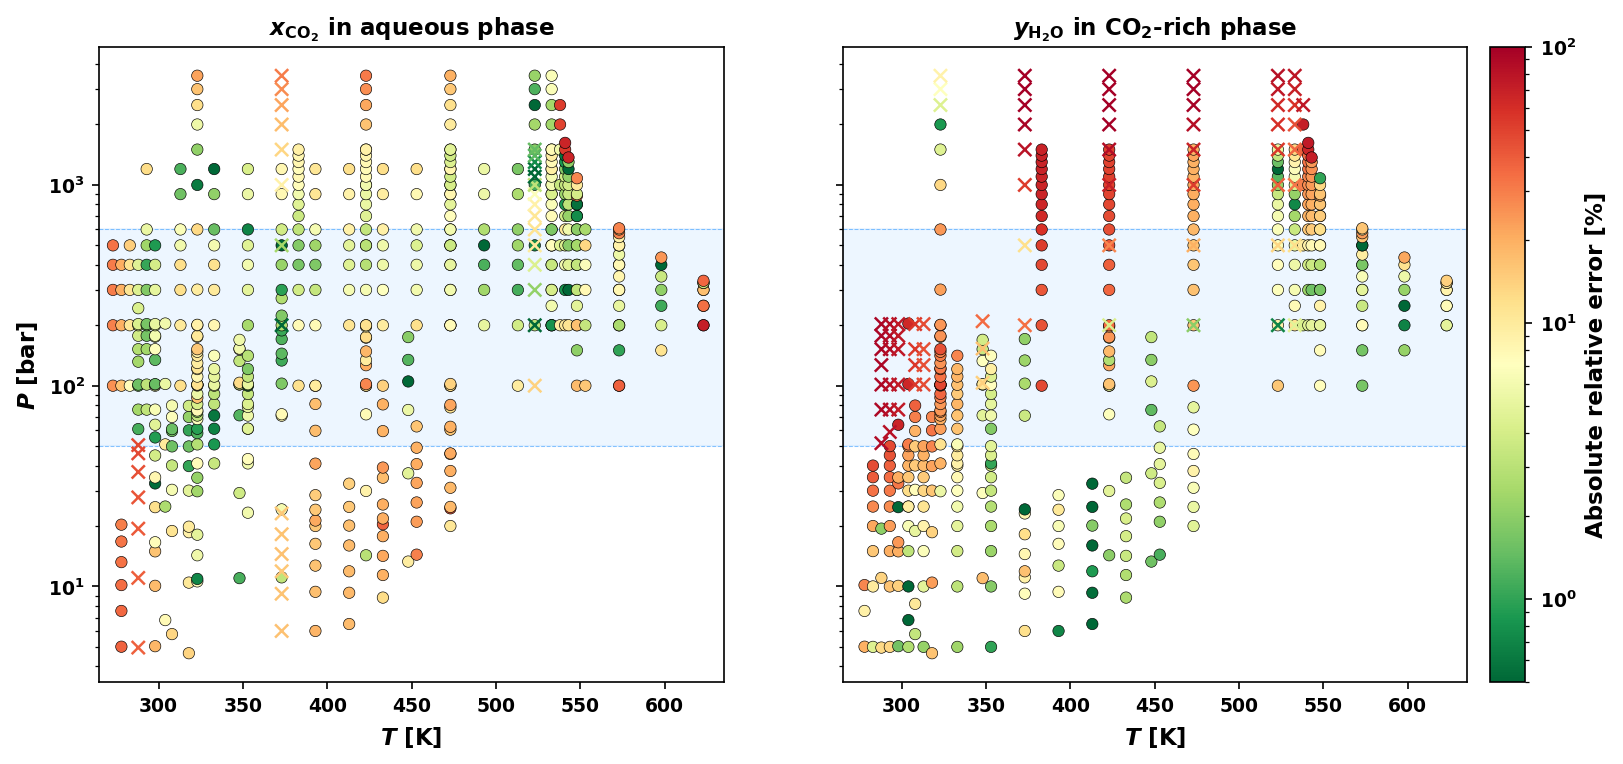
\includegraphics[width=0.95\textwidth]{fig_S6.png}
  \caption{Absolute relative error of eCPA predictions for the CO$_2$ + H$_2$O binary
           as a function of temperature and pressure.
           Left: CO$_2$ solubility in the aqueous phase ($x_{\text{CO}_2}$).
           Right: H$_2$O content in the CO$_2$-rich phase ($y_{\text{H}_2\text{O}}$).
           Marker color indicates error magnitude (green $< 5\%$, yellow $\approx 10\%$,
           red $> 30\%$); crosses mark points flagged as outliers by cross-reference
           consistency analysis.
           The blue shaded band highlights the pressure range most relevant to
           subsurface CO$_2$ storage ($P = 50$--$600$\,bar).}
  \label{fig:error_heatmap_SI}
\end{figure}

\subsection{Simplified flash: detailed accuracy and efficiency}
\label{sec:simplified_si}

Table~\ref{tab:simplified_accuracy} reports the AARE in dissolved CO$_2$ molality
$m_{\text{CO}_2}$ and the mean $y_{\text{H}_2\text{O}}$ in the CO$_2$-rich phase from the full
flash as a function of temperature, evaluated over 3{,}285 two-phase conditions
spanning $P = 25$--$800$\,bar, $z_{\text{CO}_2} = 0.01$--$0.70$, and
$m_s = 1$--$6$\,mol\,kg$^{-1}$.
The two quantities track each other closely: the simplified flash introduces an error
in $m_{\text{CO}_2}$ that equals, to a good approximation, the water content it neglects.

\begin{table}[H]
  \centering
  \caption{Accuracy of the simplified flash ($y_{\text{H}_2\text{O}} = 0$) relative to
           the full K-value SSI flash, evaluated over 3{,}285 two-phase conditions
           spanning $P = 25$--$800$\,bar, $z_{\text{CO}_2} = 0.01$--$0.70$, and
           $m_s = 1$--$6$\,mol\,kg$^{-1}$.
           AARE: average absolute relative error in CO$_2$ molality $m_{\text{CO}_2}$;
           $\langle y_{\text{H}_2\text{O}}\rangle$: mean H$_2$O mole fraction in the
           CO$_2$-rich phase from the full flash (proxy for the assumption error).}
  \label{tab:simplified_accuracy}
  \small
  \begin{tabular}{rrlrr}
    \toprule
    $T$ (K) & $T$ ($^\circ$C) & $N$ & AARE in $m_{\text{CO}_2}$ (\%) & $\langle y_{\text{H}_2\text{O}}\rangle$ (mol\%) \\
    \midrule
    283 &  10 & 239 & 0.03 & 0.02 \\
    298 &  25 & 239 & 0.11 & 0.08 \\
    313 &  40 & 240 & 0.37 & 0.27 \\
    323 &  50 & 240 & 0.62 & 0.45 \\
    333 &  60 & 240 & 0.93 & 0.68 \\
    348 &  75 & 239 & 1.55 & 1.15 \\
    353 &  80 & 240 & 1.80 & 1.34 \\
    373 & 100 & 238 & 3.16 & 2.35 \\
    393 & 120 & 239 & 5.37 & 3.91 \\
    413 & 140 & 237 & 8.95 & 6.19 \\
    423 & 150 & 237 &11.67 & 7.72 \\
    453 & 180 & 235 &25.49 &14.01 \\
    473 & 200 & 231 &45.85 &19.79 \\
    523 & 250 & 191 &121.28&33.51 \\
    \bottomrule
  \end{tabular}
\end{table}

Figure~\ref{fig:simplified_accuracy} summarises the AARE in $m_{\text{CO}_2}$, the mean
$y_{\text{H}_2\text{O}}$ from the full flash, and the wall-time speedup as functions of
temperature.
Figure~\ref{fig:simplified_by_ms} breaks the AARE down by NaCl molality; the error
curves for all salinities are nearly coincident, confirming that the accuracy of the
$y_{\text{H}_2\text{O}} = 0$ approximation is controlled entirely by temperature.

The mean wall time is essentially identical to the full flash (speedup $0.8\times$):
Brent root-finding requires on average 11.3 inner Newton evaluations, whereas the full
SSI needs 6.4 outer iterations each involving at most two inner solves.
The inner Newton cost per call is similar in both paths, so the Brent overhead offsets
the gain from eliminating the outer salt iteration.
The principal benefits of the simplified flash are therefore conceptual --- the
equilibrium reduces to a single scalar CO$_2$-solubility equation --- and robustness
in salt-free settings where the ternary outer salt loop is absent by construction.

\begin{figure}[H]
  \centering
  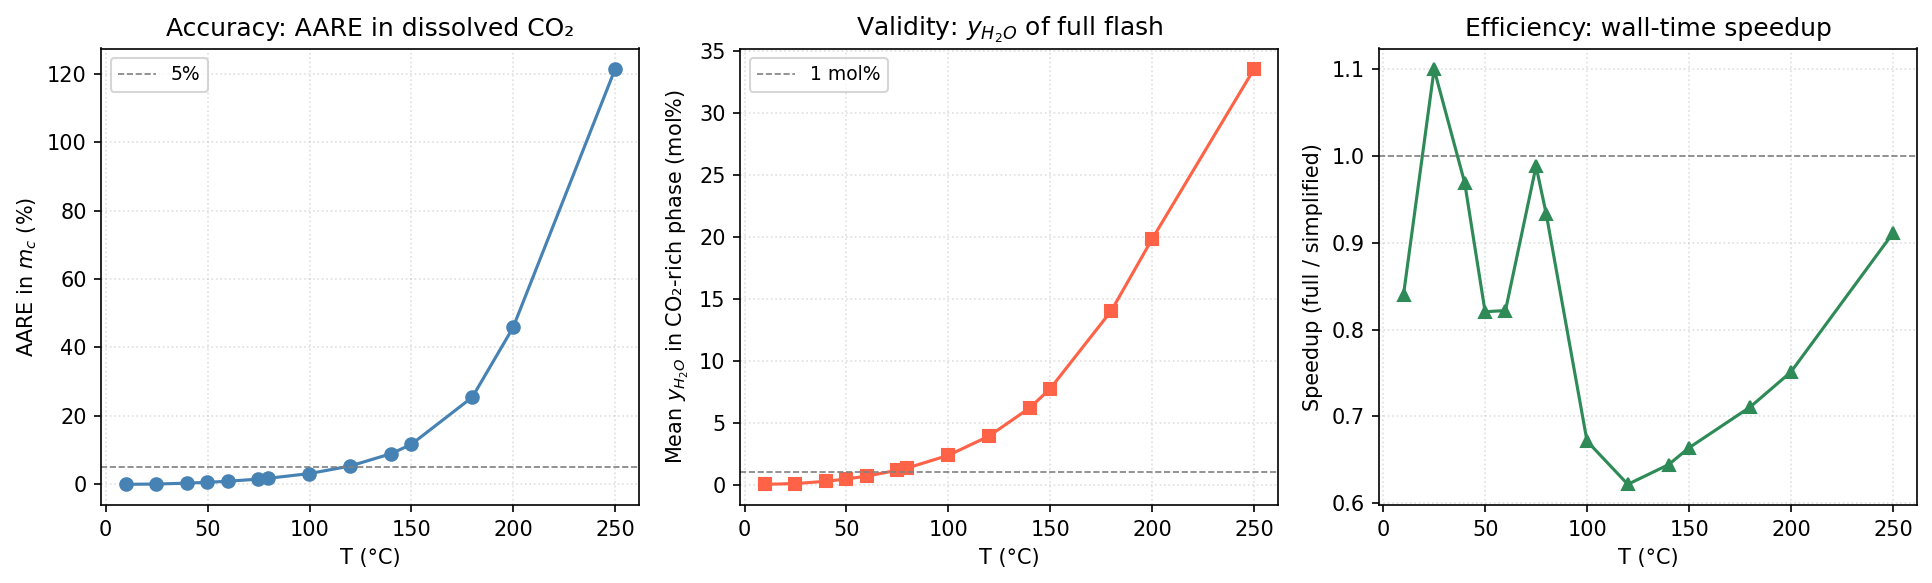
\includegraphics[width=\textwidth]{fig_11.png}
  \caption{Simplified flash benchmark over 3{,}285 two-phase conditions
           ($P = 25$--$800$\,bar; $z_{\text{CO}_2} = 0.01$--$0.70$;
           $m_s = 1$--$6$\,mol\,kg$^{-1}$).
           \textbf{Left}: AARE in dissolved CO$_2$ molality $m_{\text{CO}_2}$ as a function
           of temperature; the dashed line marks 5\%.
           \textbf{Middle}: mean H$_2$O mole fraction in the CO$_2$-rich phase
           from the full flash, which directly quantifies the magnitude of the
           $y_{\text{H}_2\text{O}} = 0$ assumption; dashed line at 1\,mol\%.
           \textbf{Right}: ratio of mean full-flash wall time to simplified-flash
           wall time; the two methods are essentially iso-cost across all temperatures.}
  \label{fig:simplified_accuracy}
\end{figure}

\begin{figure}[H]
  \centering
  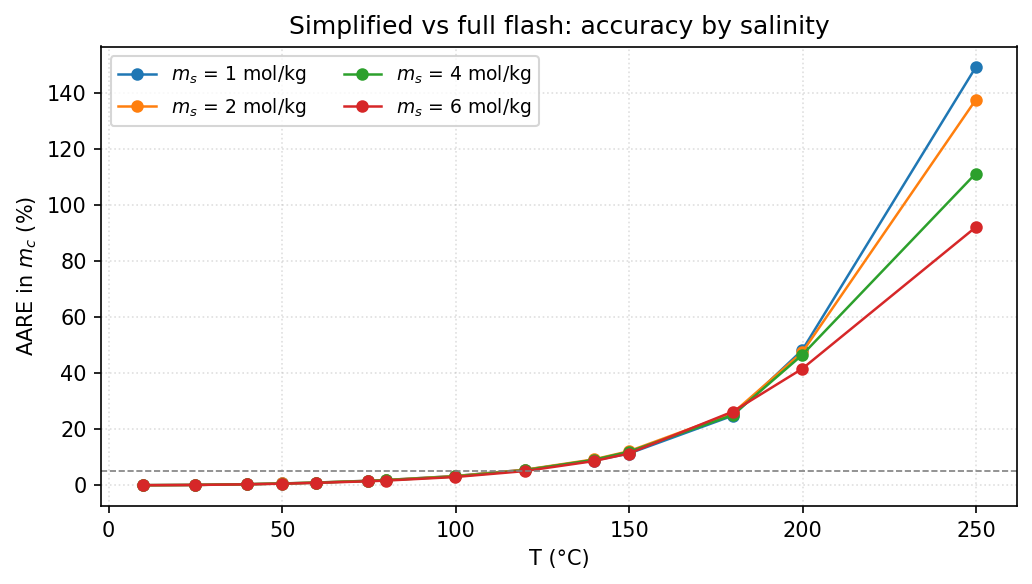
\includegraphics[width=0.65\textwidth]{fig_12.png}
  \caption{AARE in dissolved CO$_2$ molality $m_{\text{CO}_2}$ of the simplified flash versus the
           full K-value SSI, broken down by NaCl molality ($m_s = 1$--$6$\,mol\,kg$^{-1}$).
           The error curves for different salinities are nearly coincident, confirming
           that the accuracy of the $y_{\text{H}_2\text{O}} = 0$ approximation is
           controlled entirely by temperature and is insensitive to brine salinity.
           The dashed line marks 5\%.}
  \label{fig:simplified_by_ms}
\end{figure}

%% ============================================================
\section{Computational Performance Figures}
\label{sec:perf_figs_si}

This section supplements the convergence and efficiency analysis of the main text.
Figure~S10 shows the SSI+Newton iteration breakdown and wall-time ratio across the
full parameter-space scan, and Fig.~S11 compares all flash initialization strategies
in terms of convergence rate and mean iteration count.

\begin{figure}[H]
  \centering
  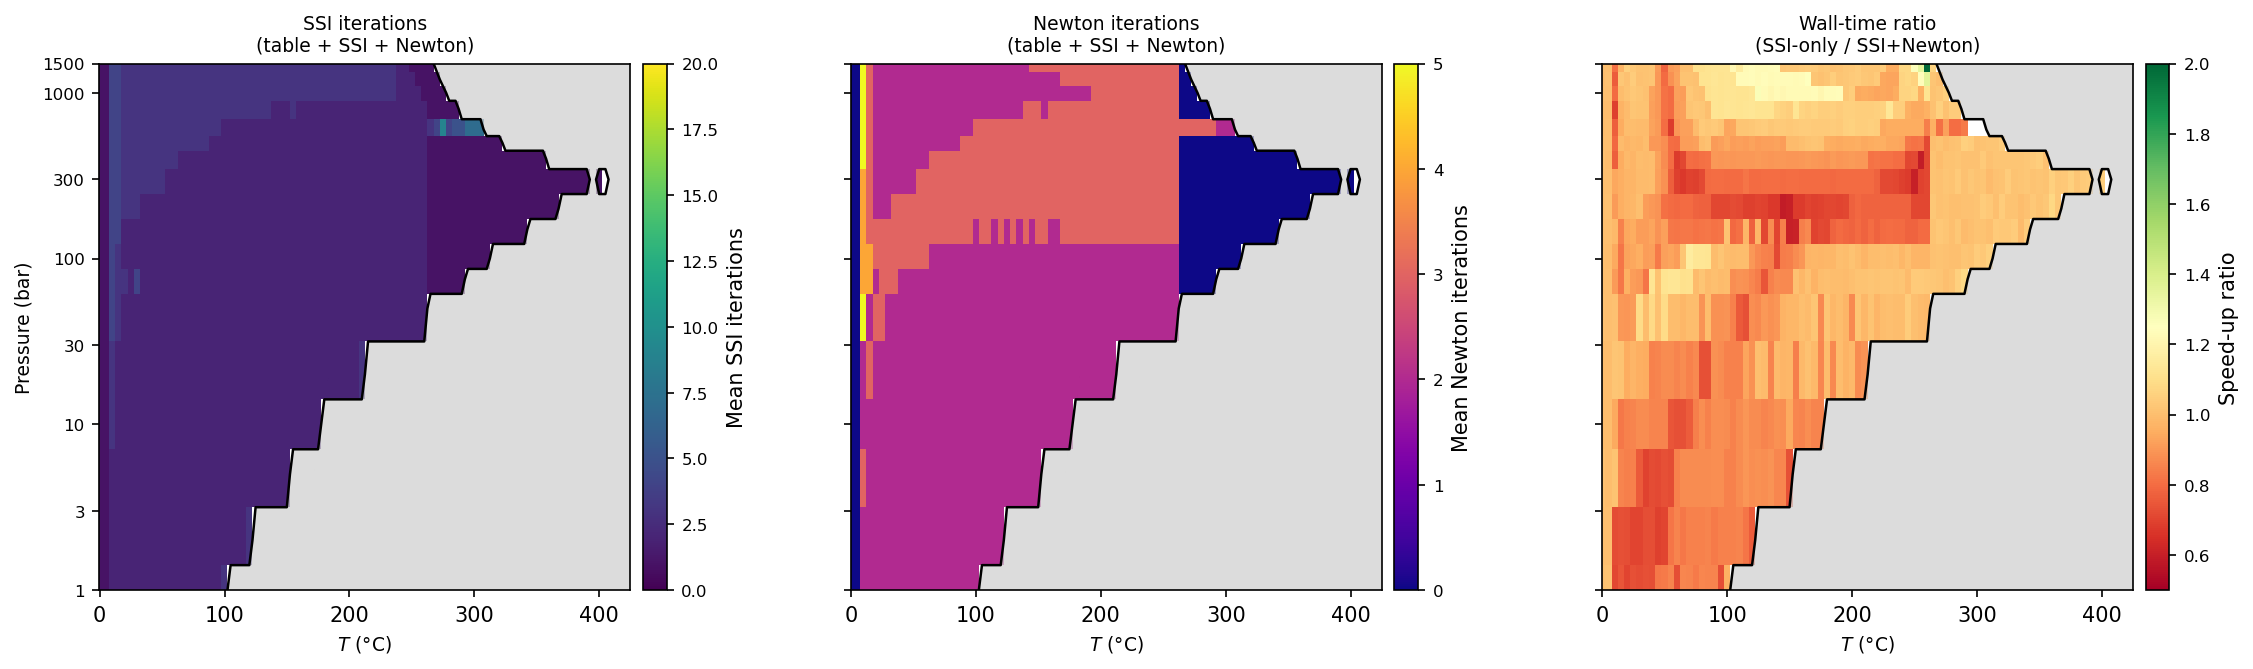
\includegraphics[width=\textwidth]{fig_S7.png}
  \caption{SSI + Newton polish iteration breakdown and wall-time ratio across the
           parameter-space scan (9{,}825 two-phase points, averaged over
           $z_{\text{CO}_2}$).
           \emph{Left}: mean SSI iteration count before Newton polish is triggered
           ($\|\mathbf{g}\| < 10^{-4}$); the near-CO$_2$-critical region
           ($T \approx 7$--$57\,^\circ$C) requires the most SSI iterations even with
           table warm-start.
           \emph{Center}: mean Newton iteration count; most of the domain converges in
           2--3 Newton steps after 1--5 SSI steps, while the critical region (blue)
           often reverts to SSI before Newton is beneficial.
           \emph{Right}: wall-time ratio (SSI-only / SSI+Newton); values $>1$ (green)
           indicate that Newton polish is faster; values $<1$ (red) indicate that the
           SSI-only path is faster (primarily near the CO$_2$ critical point where Newton
           reversion adds overhead).}
  \label{fig:newton_heatmap_SI}
\end{figure}

\begin{figure}[H]
  \centering
  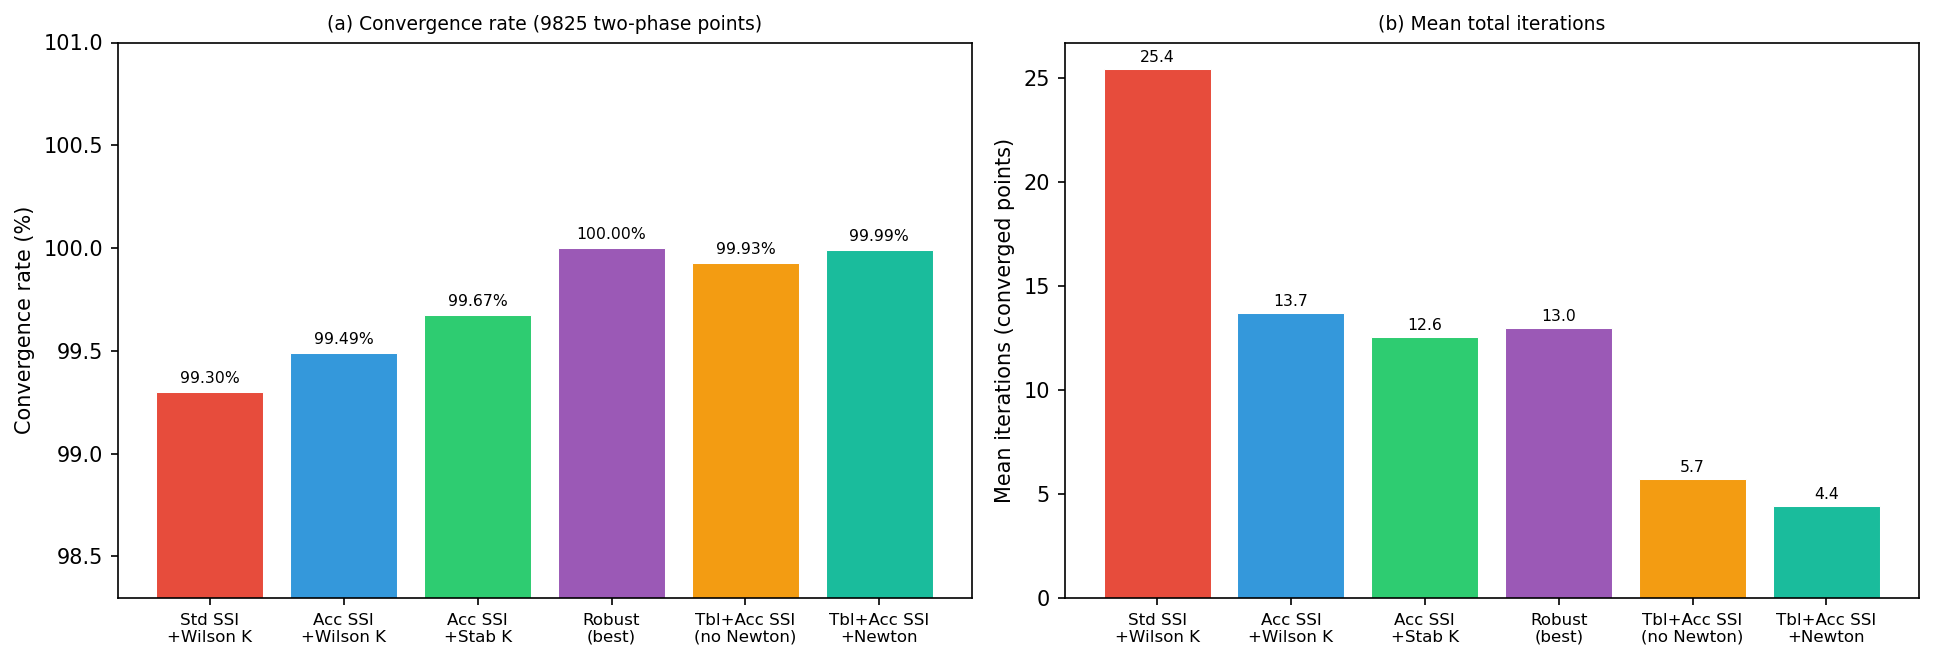
\includegraphics[width=\textwidth]{fig_S8.png}
  \caption{CPA flash strategy comparison across all 9{,}825 two-phase conditions
           of the salt-free CO$_2$ + H$_2$O parameter-space scan
           ($T = 0$--$425\,^\circ$C, $P = 1$--$1500$\,bar,
           $z_{\rm CO_2} = 0.001$--$0.999$).
           (a) Convergence rate; (b) mean total iterations (converged points only).
           Strategies are ordered from simplest cold-start (standard SSI with Wilson K)
           to the most optimized (table warm-start with SSI and Newton polish).
           The final strategy achieves a 73\% reduction in mean iterations relative to
           the standard cold-start baseline.}
  \label{fig:strategy_comparison_SI}
\end{figure}

%% ============================================================
\section{Reservoir Simulation Details}
\label{sec:sim_table}

This section supplements the reservoir simulation section of the main text, providing full
details of the numerical scheme (pressure solver, transport discretization, well model),
the complete simulation parameter set (Table~S6), spatial results and flash performance
at $t = 5$\,yr (Figs.~S12--S13; Table~S7).

\subsection*{Numerical scheme}

Pressure is solved implicitly at each time step on a uniform Cartesian grid using either
a two-point flux approximation (TPFA, \citealt{Aavatsmark2003}) or a lowest-order
mixed finite element (MFE, RT$_0$) scheme \citep{chaventjaffre}.
Both were implemented and tested; results shown here use MFE, which avoids the
pronounced grid-orientation artefacts of TPFA on Cartesian grids while remaining
computationally inexpensive \citep{moortgat2011compositional,moortgat2013higher,moortgat2016mixed}.
The solved pressure field yields Darcy velocities that drive explicit first-order upwind
advection of the overall CO$_2$ mole fraction $z_{\rm CO_2}$.
The transport sub-step size is constrained by a CFL condition based on the maximum
slope of the molar fractional flow $\partial F / \partial z_{\rm CO_2}$, estimated by a
one-dimensional scan at startup.
Production wells are controlled by a fixed bottom-hole pressure (BHP); the injector
delivers a fixed volumetric rate.

At each time step, the full Michelsen stability test followed by the two-phase flash
is called at every grid cell, using the cell pressure from the previous time step
(standard IMPES lagged-pressure).
For the eCPA case ($m_s > 0$) the warm-started K-value flash with hierarchical stability
fallback is used; for the salt-free case ($m_s = 0$) the
CPA warm-started flash is used.
NaCl is non-volatile; the equilibrium aqueous molality $m_s^\mathrm{aq}$ returned by the
flash reflects local salting-out and is used directly in the saturation calculation.

We deliberately replace the true compressible volume-rate divergence by the
incompressible constraint $\nabla\cdot\mathbf{u} = q$.
This neglects buoyancy, compressibility, and the density difference between injected and
displaced fluid.
We state this limitation explicitly because neglecting it removes the main physical driver
of CO$_2$ plume geometry in real aquifer storage, and readers should not interpret the
results as quantitative predictions.
The purpose is solely to confirm that the stability and flash routines converge reliably
and efficiently at every cell of a $50{\times}50$ grid over 300 time steps spanning
5 years.

\subsection*{Simulation setup}

Two simulations are run on identical grids with identical flow parameters, differing only
in brine salinity:
\begin{itemize}
  \item \textbf{Case A (CPA):} salt-free brine, $m_s = 0$\,mol\,kg$^{-1}$
  \item \textbf{Case B (eCPA):} saline brine, $m_s = 4$\,mol\,kg$^{-1}$ NaCl
\end{itemize}
The domain is a $100\times100$\,m$^2$ square of 10\,m thickness discretized onto a
$50\times50$ Cartesian grid ($N = 2500$ cells) with homogeneous permeability of 100\,mD
and porosity $\phi = 0.20$.
A five-spot well pattern is used: a CO$_2$ injector at the domain center and four
BHP-controlled producers at the corners (BHP $= 150$\,bar).
CO$_2$ is injected at 20\% of total pore volume per year.
The simulation runs for 5 years ($T = 77\,^\circ$C) with 300 pressure time steps.
Full simulation parameters are listed in Table~\ref{tab:sim_setup}.

\begin{table}[H]
  \centering
  \caption{Reservoir simulation parameters.}
  \label{tab:sim_setup}
  \begin{tabular}{llr}
    \toprule
    Parameter & Symbol & Value \\
    \midrule
    \multicolumn{3}{l}{\textit{Grid and geometry}} \\
    Domain size (x, y)                 & $L_x \times L_y$ & $100 \times 100$\,m \\
    Domain thickness                   & $L_z$            & 10\,m \\
    Grid cells (x, y)                  & $N_x \times N_y$ & $50 \times 50$ \\
    \midrule
    \multicolumn{3}{l}{\textit{Rock properties}} \\
    Permeability (isotropic, uniform)  & $K$              & 100\,mD \\
    Porosity                           & $\phi$           & 0.20 \\
    \midrule
    \multicolumn{3}{l}{\textit{Relative permeability (Corey)}} \\
    Connate water saturation           & $S_{wc}$         & 0.15 \\
    Residual gas saturation            & $S_{gr}$         & 0.05 \\
    End-point $k_{rg}$                 & $k_{rg}^0$       & 0.80 \\
    End-point $k_{rw}$                 & $k_{rw}^0$       & 1.00 \\
    Corey exponent (CO$_2$-rich phase) & $n_g$            & 2.0  \\
    Corey exponent (aqueous phase)     & $n_w$            & 2.5  \\
    \midrule
    \multicolumn{3}{l}{\textit{Fluid properties}} \\
    Temperature (isothermal)           & $T$              & $77\,^\circ$C (350\,K) \\
    CO$_2$-rich phase viscosity        & $\mu_g$          & $5\times10^{-5}$\,Pa\,s \\
    Aqueous phase viscosity            & $\mu_w$          & $4.5\times10^{-4}$\,Pa\,s \\
    \midrule
    \multicolumn{3}{l}{\textit{Well and injection parameters}} \\
    Well pattern                       & ---              & five-spot \\
    Injector location                  & ---              & domain center \\
    Producer locations                 & ---              & four corners \\
    Wellbore radius                    & $r_w$            & 0.10\,m \\
    Producer BHP                       & $P_\mathrm{BHP}$ & 150\,bar \\
    Injection rate                     & ---              & 20\% PVI\,yr$^{-1}$ \\
    \midrule
    \multicolumn{3}{l}{\textit{Simulation control}} \\
    Total simulation time              & $t_\mathrm{max}$ & 5\,yr \\
    Number of pressure time steps      & $N_t$            & 300 \\
    Pressure solver                    & ---              & MFE (RT$_0$) \\
    Transport scheme                   & ---              & first-order upwind, CFL-limited \\
    \midrule
    \multicolumn{3}{l}{\textit{Cases}} \\
    Case A (CPA)                       & $m_s$            & $0$\,mol\,kg$^{-1}$ (salt-free) \\
    Case B (eCPA)                      & $m_s$            & $4$\,mol\,kg$^{-1}$ NaCl \\
    \bottomrule
  \end{tabular}
\end{table}

\subsection*{Results}

Figure~\ref{fig:sim_comparison} shows the final-time ($t = 5$\,yr) spatial fields for
both cases: the CO$_2$-rich saturation $S_g$ (top row), the dissolved CO$_2$ molality
$m_{\text{CO}_2}$ in the aqueous phase (middle row), and the pressure field (bottom row).
The CO$_2$ saturation maps are strikingly similar between the two cases.
This is physically expected: at a high injection rate of 20\% PVI\,yr$^{-1}$, advection
strongly dominates over dissolution-driven transport.
The CO$_2$ displacement front is governed primarily by the mobility ratio and the
imposed pressure gradient, not by whether the equilibrium CO$_2$ solubility in the
aqueous phase is slightly reduced by salt.
Given that CO$_2$ solubility in water is already low---on the order of
1--2\,mol\,kg$^{-1}$ under typical storage conditions---the further reduction from
salting-out has negligible impact on the high-rate displacement dynamics on these
time scales.

The dissolved CO$_2$ maps (middle row) tell a different story.
Inside the plume the aqueous phase is everywhere CO$_2$-saturated at the local
equilibrium value: $m_{\text{CO}_2} \approx 1.25$\,mol\,kg$^{-1}$ for the salt-free case
and only $m_{\text{CO}_2} \approx 0.63$\,mol\,kg$^{-1}$ at $m_s = 4$\,mol\,kg$^{-1}$---a
reduction of approximately a factor of two, consistent with the salting-out effect
seen in the validation data.
The white region around the central injector marks cells where the brine has been fully
expelled into the CO$_2$-rich phase (complete drying out, $S_g \to 1$), despite a 15\%
connate/residual water saturation.
Correctly capturing this drying-out regime requires a robust stability and flash model
that fully captures the mutual solubilities of CO$_2$ and H$_2$O.

No flash failures were recorded in either simulation across all 300 time steps and
all 2500 grid cells, confirming the reliability of the hierarchical stability and flash
approach.

\begin{figure}[H]
  \centering
  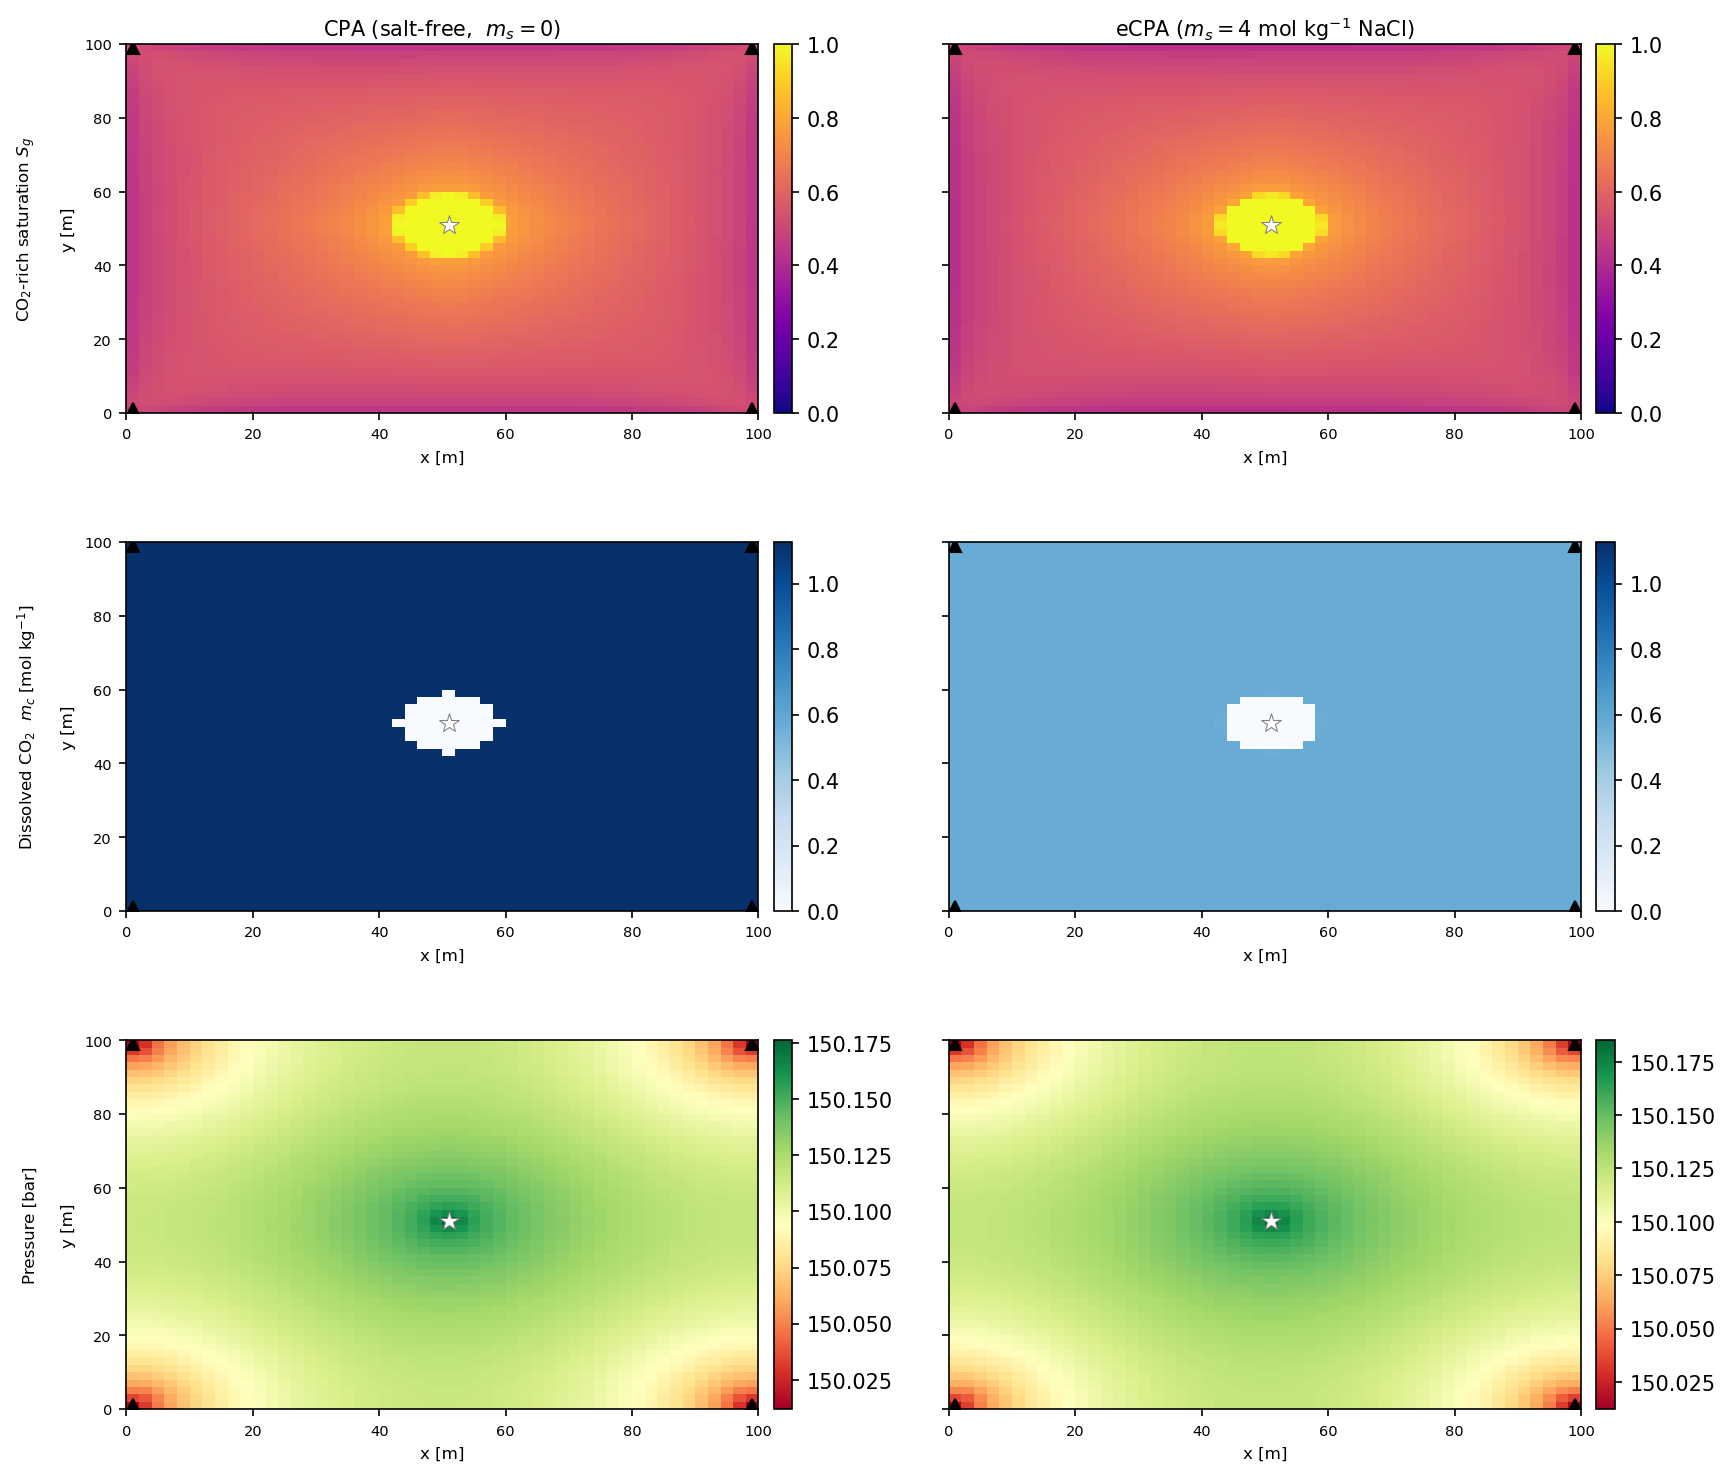
\includegraphics[width=\textwidth]{fig_10.png}
  \caption{Final-state ($t = 5$\,yr) spatial fields for the salt-free CPA case
           ($m_s = 0$, left column) and the saline eCPA case
           ($m_s = 4$\,mol\,kg$^{-1}$ NaCl, right column).
           \emph{Top row}: CO$_2$-rich phase saturation $S_g$.
           The plumes are nearly identical, reflecting advection-dominated displacement
           at 20\% PVI\,yr$^{-1}$.
           \emph{Middle row}: dissolved CO$_2$ molality $m_{\text{CO}_2}$ in the aqueous phase.
           Inside the plume the aqueous phase is CO$_2$-saturated at the eCPA
           equilibrium value: ${\approx}1.25$\,mol\,kg$^{-1}$ (salt-free) vs.\
           ${\approx}0.63$\,mol\,kg$^{-1}$ ($m_s = 4$\,mol\,kg$^{-1}$), a factor-of-two
           reduction from the salting-out effect.
           The white region near the central injector (white star) marks cells where
           brine has been completely expelled into the CO$_2$-rich phase (drying-out).
           \emph{Bottom row}: pressure field; the ${\approx}0.15$\,bar gradient across
           the 100\,m domain reflects the small pressure drop required to drive
           20\% PVI\,yr$^{-1}$ through 100\,mD rock with BHP-controlled producers at
           150\,bar.
           Black triangles: producers.}
  \label{fig:sim_comparison}
\end{figure}

While the saturation fields are similar, the implications for long-term CO$_2$ storage
are markedly different.
Solubility trapping---the dissolution of CO$_2$ into the formation brine---is a key
mechanism for storage permanence, because dissolved CO$_2$ cannot escape as a
buoyant supercritical phase.
Figure~\ref{fig:sim_trapping} shows the fraction of the in-situ CO$_2$ inventory that
is dissolved in brine (solubility trapping, solid lines) versus residing in the
CO$_2$-rich phase (structural trapping, dashed lines) as a function of time for both
cases.
The gap between the CPA and eCPA curves is clear and persistent throughout: at $t = 5$\,yr
the solubility trapping fraction is roughly a factor of two lower for the saline case,
directly reflecting the reduction in equilibrium CO$_2$ solubility from the salting-out
effect.
This demonstrates that brine salinity has a quantitatively significant impact on
long-term storage permanence even when the short-term displacement dynamics appear
unaffected.

\subsection*{Flash performance in the simulator}

At every time step, the stability test and flash are called at each of the $N = 2500$
grid cells.
Cells identified as trivially single-phase bypass the flash entirely; the remaining
two-phase candidates are dispatched in parallel across all available CPU cores.
As the plume grows, an increasing fraction of the domain becomes two-phase until
essentially all cells require a flash call (peak ${\approx}2500$ calls per step).
Performance numbers for both simulations are summarized in Table~\ref{tab:sim_perf};
the flash accounts for the dominant fraction of total step cost throughout both runs,
confirming that the algorithmic efficiency of the warm-started flash directly governs
simulation throughput.
Interestingly, the eCPA flash achieves a higher throughput than CPA (14{,}270 vs.\
8{,}840\,calls\,s$^{-1}$), even though the eCPA EoS involves more unknowns and is
inherently more expensive per iteration.
While one would expect CPA to be the faster of the two in general, the solution-table
warm start appears to provide particularly accurate initial guesses for the eCPA system
at the temperature, pressure, and salinity conditions of these simulations
($T = 77\,^\circ$C, $P \approx 150$\,bar, $m_s = 4$\,mol\,kg$^{-1}$), resulting in
fewer SSI iterations to convergence than for the salt-free CPA case at otherwise
identical conditions.

\begin{table}[H]
  \centering
  \caption{Aggregate flash performance for the 5-year simulations
           ($50\times50$ grid, $T = 77\,^\circ$C, $P \approx 150$\,bar, 300 time steps,
           48 CPU cores). Total wall time: 91\,s (CPA) and 63\,s (eCPA).}
  \label{tab:sim_perf}
  \begin{tabular}{lrr}
    \toprule
    Metric & CPA ($m_s = 0$) & eCPA ($m_s = 4$) \\
    \midrule
    Grid cells                          & 2500       & 2500       \\
    Time steps                          & 300        & 300        \\
    Mean two-phase cells / step         & 2219 (max 2479) & 2213 (max 2479) \\
    Mean flash wall time / step (s)     & 0.247      & 0.151      \\
    Flash fraction of step cost         & 87\%       & 80\%       \\
    Flash throughput (calls\,s$^{-1}$)  & 8{,}840    & 14{,}270   \\
    \bottomrule
  \end{tabular}
\end{table}

\begin{figure}[H]
  \centering
  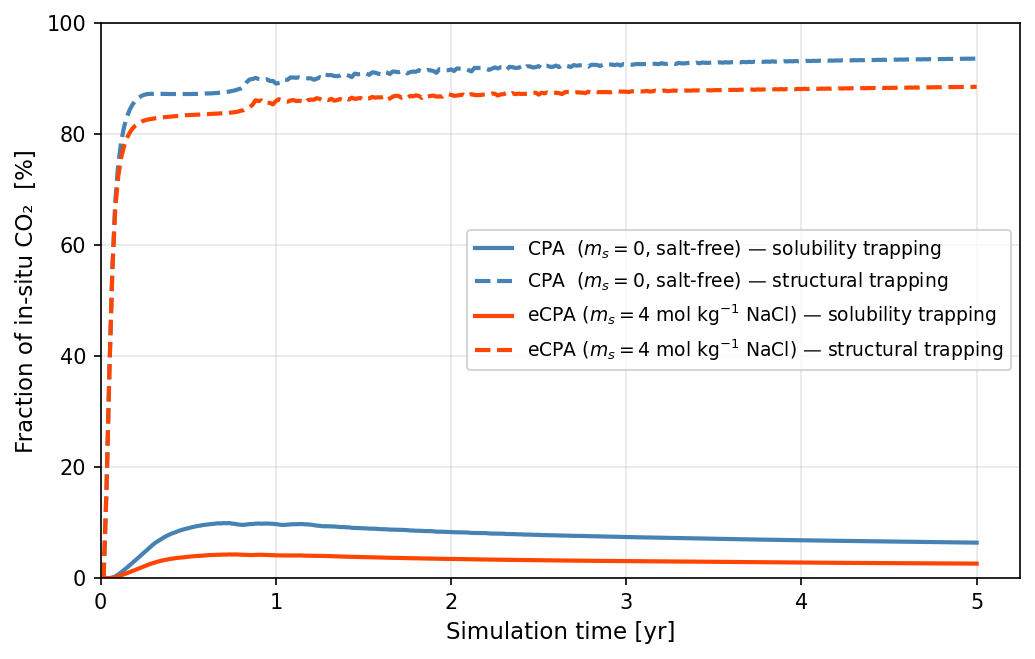
\includegraphics[width=0.80\textwidth]{fig_S9.png}
  \caption{Fraction of total in-situ CO$_2$ inventory undergoing solubility trapping
           (dissolved in the aqueous phase, solid lines) versus structural trapping
           (residing in the CO$_2$-rich phase, dashed lines) as a function of time.
           Blue: salt-free brine (CPA, $m_s = 0$);
           red: saline brine (eCPA, $m_s = 4$\,mol\,kg$^{-1}$ NaCl).
           The persistent factor-of-two gap in solubility trapping between the two cases
           reflects the reduction in equilibrium CO$_2$ solubility due to the
           salting-out effect, which has negligible impact on short-term displacement
           dynamics but is critical for long-term storage permanence.}
  \label{fig:sim_trapping}
\end{figure}

%% ============================================================
\begin{thebibliography}{21}
\expandafter\ifx\csname natexlab\endcsname\relax\def\natexlab#1{#1}\fi
\providecommand{\url}[1]{\texttt{#1}}
\providecommand{\href}[2]{#2}
\providecommand{\path}[1]{#1}
\providecommand{\DOIprefix}{doi:}
\providecommand{\ArXivprefix}{arXiv:}
\providecommand{\URLprefix}{URL: }
\providecommand{\Pubmedprefix}{pmid:}
\providecommand{\doi}[1]{\href{http://dx.doi.org/#1}{\path{#1}}}
\providecommand{\Pubmed}[1]{\href{pmid:#1}{\path{#1}}}
\providecommand{\bibinfo}[2]{#2}
\ifx\xfnm\relax \def\xfnm[#1]{\unskip,\space#1}\fi
%Type = Article
\bibitem[{Aavatsmark(2002)}]{Aavatsmark2003}
\bibinfo{author}{Aavatsmark, I.}, \bibinfo{year}{2002}.
\newblock \bibinfo{title}{An introduction to multipoint flux approximations for
  quadrilateral grids}.
\newblock \bibinfo{journal}{Comput. Geosci.} \bibinfo{volume}{6},
  \bibinfo{pages}{405--432}.
%Type = Article
\bibitem[{Bando et~al.(2003)Bando, Takemura, Nishio, Hihara and
  Akai}]{Bando2003}
\bibinfo{author}{Bando, S.}, \bibinfo{author}{Takemura, F.},
  \bibinfo{author}{Nishio, M.}, \bibinfo{author}{Hihara, E.},
  \bibinfo{author}{Akai, M.}, \bibinfo{year}{2003}.
\newblock \bibinfo{title}{Solubility of \ce{CO2} in aqueous solutions of nacl
  at (30 to 60) °c and (10 to 20) mpa}.
\newblock \bibinfo{journal}{Journal of Chemical \& Engineering Data}
  \bibinfo{volume}{48}, \bibinfo{pages}{576--579}.
%Type = Article
\bibitem[{Chabab et~al.(2020)Chabab, Théveneau, Coquelet, Corvisier and
  Fossion}]{Chabab2020}
\bibinfo{author}{Chabab, S.}, \bibinfo{author}{Théveneau, P.},
  \bibinfo{author}{Coquelet, C.}, \bibinfo{author}{Corvisier, J.},
  \bibinfo{author}{Fossion, P.}, \bibinfo{year}{2020}.
\newblock \bibinfo{title}{Measurements and predictive models of high-pressure
  {H$_2$S} solubility in brine ({NaCl} aqueous solution) and mixed gas
  ({CO$_2$} + {H$_2$S}) solubilities in various aqueous solutions at high
  pressures}.
\newblock \bibinfo{journal}{Int. J. Greenhouse Gas Control}
  \bibinfo{volume}{93}, \bibinfo{pages}{102894}.
\newblock \DOIprefix\doi{10.1016/j.ijggc.2019.102894}. \bibinfo{note}{cO$_2$ +
  NaCl data at $m_s = 6$\,mol\,kg$^{-1}$}.
%Type = Book
\bibitem[{Chavent and Jaffre(1986)}]{chaventjaffre}
\bibinfo{author}{Chavent, G.}, \bibinfo{author}{Jaffre, J.},
  \bibinfo{year}{1986}.
\newblock \bibinfo{title}{{Mathematical models and finite elements for
  reservoir simulation. Studies in mathematics and its applications.}}
\newblock \bibinfo{publisher}{Elsevier}, \bibinfo{address}{North-Holland}.
%Type = Article
\bibitem[{Coelho et~al.(2025)Coelho, Franco and Firoozabadi}]{Coelho2025}
\bibinfo{author}{Coelho, F.M.}, \bibinfo{author}{Franco, L.F.M.},
  \bibinfo{author}{Firoozabadi, A.}, \bibinfo{year}{2025}.
\newblock \bibinfo{title}{Phase equilibria of {CO$_2$}--water and
  {CO$_2$}--brine at high temperatures: From {Monte Carlo} simulations to the
  equation of state}.
\newblock \bibinfo{journal}{Ind. Eng. Chem. Res.} \bibinfo{volume}{64},
  \bibinfo{pages}{8492--8505}.
\newblock \DOIprefix\doi{10.1021/acs.iecr.5c00134}.
%Type = Article
\bibitem[{Guo et~al.(2015)Guo, Huang, Chen and Zhou}]{Guo2015}
\bibinfo{author}{Guo, H.}, \bibinfo{author}{Huang, Y.}, \bibinfo{author}{Chen,
  Y.}, \bibinfo{author}{Zhou, Q.}, \bibinfo{year}{2015}.
\newblock \bibinfo{title}{Quantitative {Raman} spectroscopic measurements of
  {CO$_2$} solubility in {NaCl} solution from 273.15 to 473.15 {K} at {$p$ = 10
  to 100 MPa}}.
\newblock \bibinfo{journal}{J. Chem. Eng. Data} \bibinfo{volume}{61},
  \bibinfo{pages}{466--474}.
\newblock \DOIprefix\doi{10.1021/acs.jced.5b00799}.
%Type = Article
\bibitem[{Hou et~al.(2013)Hou, Maitland and Trusler}]{Hou2013}
\bibinfo{author}{Hou, S.X.}, \bibinfo{author}{Maitland, G.C.},
  \bibinfo{author}{Trusler, J.P.M.}, \bibinfo{year}{2013}.
\newblock \bibinfo{title}{Measurement and modeling of the phase behavior of the
  ({Carbon Dioxide} + {Water}) and ({Carbon Dioxide} + {Water} + {NaCl})
  systems at temperatures from 298.15 to 448.15 {K}}.
\newblock \bibinfo{journal}{J. Supercrit. Fluids} \bibinfo{volume}{73},
  \bibinfo{pages}{87--96}.
\newblock \DOIprefix\doi{10.1016/j.supflu.2012.11.011}.
%Type = Article
\bibitem[{Koschel et~al.(2006)Koschel, Coxam, Rodier and Majer}]{Koschel2006}
\bibinfo{author}{Koschel, D.}, \bibinfo{author}{Coxam, J.Y.},
  \bibinfo{author}{Rodier, L.}, \bibinfo{author}{Majer, V.},
  \bibinfo{year}{2006}.
\newblock \bibinfo{title}{Enthalpy and solubility data of {CO$_2$} in water and
  {NaCl(aq)} at conditions of interest for geological sequestration}.
\newblock \bibinfo{journal}{Fluid Phase Equilib.} \bibinfo{volume}{247},
  \bibinfo{pages}{107--120}.
\newblock \DOIprefix\doi{10.1016/j.fluid.2006.06.016}.
%Type = Article
\bibitem[{Liu et~al.(2021)Liu, Mahmood, Mohammadian, Khaksar~Manshad, Rosli and
  Ostadhassan}]{Liu2021}
\bibinfo{author}{Liu, B.}, \bibinfo{author}{Mahmood, B.S.},
  \bibinfo{author}{Mohammadian, E.}, \bibinfo{author}{Khaksar~Manshad, A.},
  \bibinfo{author}{Rosli, N.R.}, \bibinfo{author}{Ostadhassan, M.},
  \bibinfo{year}{2021}.
\newblock \bibinfo{title}{Measurement of solubility of \ce{CO2} in nacl,
  \ce{CaCl2}, \ce{MgCl2} and \ce{MgCl2} + \ce{CaCl2} brines at temperatures
  from 298 to 373 k and pressures up to 20 mpa using the potentiometric
  titration method}.
\newblock \bibinfo{journal}{Energies} \bibinfo{volume}{14},
  \bibinfo{pages}{7222}.
\newblock \URLprefix \url{https://www.mdpi.com/1996-1073/14/21/7222}.
%Type = Article
\bibitem[{Liu et~al.(2011)Liu, Hou, Yang and Han}]{Liu2011b}
\bibinfo{author}{Liu, Y.}, \bibinfo{author}{Hou, M.}, \bibinfo{author}{Yang,
  G.}, \bibinfo{author}{Han, B.}, \bibinfo{year}{2011}.
\newblock \bibinfo{title}{Solubility of \ce{CO2} in aqueous solutions of nacl,
  kcl, \ce{CaCl2} and their mixed salts at different temperatures and
  pressures}.
\newblock \bibinfo{journal}{The Journal of Supercritical Fluids}
  \bibinfo{volume}{56}, \bibinfo{pages}{125--129}.
%Type = Article
\bibitem[{Messabeb et~al.(2016)Messabeb, Contamine, Cézac, Serin and
  Gaucher}]{Messabeb2016}
\bibinfo{author}{Messabeb, H.}, \bibinfo{author}{Contamine, F.},
  \bibinfo{author}{Cézac, P.}, \bibinfo{author}{Serin, J.P.},
  \bibinfo{author}{Gaucher, E.C.}, \bibinfo{year}{2016}.
\newblock \bibinfo{title}{Experimental measurement of {CO$_2$} solubility in
  aqueous {NaCl} solution at temperature from 323.15 to 423.15 {K} and pressure
  of up to 20 {MPa}}.
\newblock \bibinfo{journal}{J. Chem. Eng. Data} \bibinfo{volume}{61},
  \bibinfo{pages}{3573--3584}.
\newblock \DOIprefix\doi{10.1021/acs.jced.6b00505}.
%Type = Article
\bibitem[{Moortgat and Firoozabadi(2013)}]{moortgat2013higher}
\bibinfo{author}{Moortgat, J.}, \bibinfo{author}{Firoozabadi, A.},
  \bibinfo{year}{2013}.
\newblock \bibinfo{title}{Higher-order compositional modeling of three-phase
  flow in 3d fractured porous media based on cross-flow equilibrium}.
\newblock \bibinfo{journal}{Journal of Computational Physics}
  \bibinfo{volume}{250}, \bibinfo{pages}{425--445}.
%Type = Article
\bibitem[{Moortgat and Firoozabadi(2016)}]{moortgat2016mixed}
\bibinfo{author}{Moortgat, J.}, \bibinfo{author}{Firoozabadi, A.},
  \bibinfo{year}{2016}.
\newblock \bibinfo{title}{Mixed-hybrid and vertex-discontinuous-galerkin finite
  element modeling of multiphase compositional flow on 3d unstructured grids}.
\newblock \bibinfo{journal}{Journal of Computational Physics}
  \bibinfo{volume}{315}, \bibinfo{pages}{476--500}.
%Type = Article
\bibitem[{Moortgat et~al.(2011)Moortgat, Sun and
  Firoozabadi}]{moortgat2011compositional}
\bibinfo{author}{Moortgat, J.}, \bibinfo{author}{Sun, S.},
  \bibinfo{author}{Firoozabadi, A.}, \bibinfo{year}{2011}.
\newblock \bibinfo{title}{Compositional modeling of three-phase flow with
  gravity using higher-order finite element methods}.
\newblock \bibinfo{journal}{Water Resources Research} \bibinfo{volume}{47}.
%Type = Article
\bibitem[{Nighswander et~al.(1989)Nighswander, Kalogerakis and
  Mehrotra}]{Nighswander1989}
\bibinfo{author}{Nighswander, J.A.}, \bibinfo{author}{Kalogerakis, N.},
  \bibinfo{author}{Mehrotra, A.K.}, \bibinfo{year}{1989}.
\newblock \bibinfo{title}{Solubilities of carbon dioxide in water and 1 wt.\ \%
  {NaCl} solution at pressures up to 10 {MPa} and temperatures from 80 to 200
  {$^\circ$C}}.
\newblock \bibinfo{journal}{J. Chem. Eng. Data} \bibinfo{volume}{34},
  \bibinfo{pages}{355--360}.
\newblock \DOIprefix\doi{10.1021/je00057a027}.
%Type = Article
\bibitem[{Rumpf et~al.(1994)Rumpf, Nicolaisen, Öcal and Maurer}]{Rumpf1994}
\bibinfo{author}{Rumpf, B.}, \bibinfo{author}{Nicolaisen, H.},
  \bibinfo{author}{Öcal, C.}, \bibinfo{author}{Maurer, G.},
  \bibinfo{year}{1994}.
\newblock \bibinfo{title}{Solubility of carbon dioxide in aqueous solutions of
  sodium chloride: Experimental results and correlation}.
\newblock \bibinfo{journal}{J. Solution Chem.} \bibinfo{volume}{23},
  \bibinfo{pages}{431--448}.
\newblock \DOIprefix\doi{10.1007/BF00973113}.
%Type = Article
\bibitem[{Savary et~al.(2012)Savary, Berger, Dubois, Lacharpagne, Pages,
  Thibeau and Lescanne}]{Savary2012}
\bibinfo{author}{Savary, V.}, \bibinfo{author}{Berger, G.},
  \bibinfo{author}{Dubois, M.}, \bibinfo{author}{Lacharpagne, J.C.},
  \bibinfo{author}{Pages, A.}, \bibinfo{author}{Thibeau, S.},
  \bibinfo{author}{Lescanne, M.}, \bibinfo{year}{2012}.
\newblock \bibinfo{title}{The solubility of \ce{CO2}+\ce{H2S} mixtures in water
  and 2m nacl at 120°c and pressures up to 35mpa}.
\newblock \bibinfo{journal}{International Journal of Greenhouse Gas Control}
  \bibinfo{volume}{10}, \bibinfo{pages}{123--133}.
%Type = Article
\bibitem[{Takenouchi and Kennedy(1965)}]{Takenouchi1965}
\bibinfo{author}{Takenouchi, S.}, \bibinfo{author}{Kennedy, G.C.},
  \bibinfo{year}{1965}.
\newblock \bibinfo{title}{The solubility of carbon dioxide in {NaCl} solutions
  at high temperatures and pressures}.
\newblock \bibinfo{journal}{Am. J. Sci.} \bibinfo{volume}{263},
  \bibinfo{pages}{445--454}.
\newblock \DOIprefix\doi{10.2475/ajs.263.5.445}.
%Type = Article
\bibitem[{Wagner and Pru{\ss}(2002)}]{IAPWS2016}
\bibinfo{author}{Wagner, W.}, \bibinfo{author}{Pru{\ss}, A.},
  \bibinfo{year}{2002}.
\newblock \bibinfo{title}{The {IAPWS} formulation 1995 for the thermodynamic
  properties of ordinary water substance for general and scientific use}.
\newblock \bibinfo{journal}{Journal of Physical and Chemical Reference Data}
  \bibinfo{volume}{31}, \bibinfo{pages}{387--535}.
\newblock \DOIprefix\doi{10.1063/1.1461829}. \bibinfo{note}{iAPWS-95; revised
  release 2016}.
%Type = Article
\bibitem[{Yan et~al.(2011)Yan, Huang and Stenby}]{Yan2011}
\bibinfo{author}{Yan, W.}, \bibinfo{author}{Huang, S.},
  \bibinfo{author}{Stenby, E.H.}, \bibinfo{year}{2011}.
\newblock \bibinfo{title}{Measurement and modeling of {CO$_2$} solubility in
  {NaCl} brine and {CO$_2$} + {NaCl} brine + {CH$_4$} systems}.
\newblock \bibinfo{journal}{Int. J. Greenhouse Gas Control}
  \bibinfo{volume}{5}, \bibinfo{pages}{1460--1477}.
\newblock \DOIprefix\doi{10.1016/j.ijggc.2011.08.004}.
%Type = Article
\bibitem[{Zhao et~al.(2015)Zhao, Dilmore, Allen, Hedges, Soong and
  Lvov}]{Zhao2015}
\bibinfo{author}{Zhao, H.}, \bibinfo{author}{Dilmore, R.},
  \bibinfo{author}{Allen, D.E.}, \bibinfo{author}{Hedges, S.W.},
  \bibinfo{author}{Soong, Y.}, \bibinfo{author}{Lvov, S.N.},
  \bibinfo{year}{2015}.
\newblock \bibinfo{title}{Measurement and model predictions of solubility of
  {CO$_2$} in {NaCl} aqueous solution at temperatures from 323 to 423 {K} and
  pressures up to 40 {MPa}}.
\newblock \bibinfo{journal}{Int. J. Greenhouse Gas Control}
  \bibinfo{volume}{37}, \bibinfo{pages}{59--69}.
\newblock \DOIprefix\doi{10.1016/j.ijggc.2015.02.008}.

\end{thebibliography}

\end{document}
